\chapter{Choosing an Estimator}\label{ch:T5}

\providecommand{\TFiveALabN}{}\renewcommand{\TFiveALabN}{25}
\providecommand{\TFiveALabM}{}\renewcommand{\TFiveALabM}{20000}
\providecommand{\TFiveALabCore}{}\renewcommand{\TFiveALabCore}{0.410}
\providecommand{\TFiveALabAMean}{}\renewcommand{\TFiveALabAMean}{1.014}
\providecommand{\TFiveALabAMed}{}\renewcommand{\TFiveALabAMed}{1.544}
\providecommand{\TFiveALabAML}{}\renewcommand{\TFiveALabAML}{1.014}
\providecommand{\TFiveALabAMedTh}{}\renewcommand{\TFiveALabAMedTh}{1.571}
\providecommand{\TFiveALabACR}{}\renewcommand{\TFiveALabACR}{1.000}
\providecommand{\TFiveALabBMean}{}\renewcommand{\TFiveALabBMean}{1.008}
\providecommand{\TFiveALabBMed}{}\renewcommand{\TFiveALabBMed}{0.673}
\providecommand{\TFiveALabBML}{}\renewcommand{\TFiveALabBML}{0.672}
\providecommand{\TFiveALabBMedTh}{}\renewcommand{\TFiveALabBMedTh}{0.500}
\providecommand{\TFiveALabBCR}{}\renewcommand{\TFiveALabBCR}{0.500}
\providecommand{\TFiveALabCMean}{}\renewcommand{\TFiveALabCMean}{1.005}
\providecommand{\TFiveALabCMed}{}\renewcommand{\TFiveALabCMed}{0.291}
\providecommand{\TFiveALabCML}{}\renewcommand{\TFiveALabCML}{0.191}
\providecommand{\TFiveALabCMedTh}{}\renewcommand{\TFiveALabCMedTh}{0.289}
\providecommand{\TFiveALabCCR}{}\renewcommand{\TFiveALabCCR}{0.186}
\providecommand{\TFiveALabCInfo}{}\renewcommand{\TFiveALabCInfo}{5.386}
\providecommand{\TFiveALabCfzero}{}\renewcommand{\TFiveALabCfzero}{0.9293}
\providecommand{\TFiveALabCGain}{}\renewcommand{\TFiveALabCGain}{3.46}
\providecommand{\TFiveAWeighM}{}\renewcommand{\TFiveAWeighM}{200000}
\providecommand{\TFiveAWeighSigma}{}\renewcommand{\TFiveAWeighSigma}{0.1}
\providecommand{\TFiveAWeighVBlue}{}\renewcommand{\TFiveAWeighVBlue}{0.6716}
\providecommand{\TFiveAWeighVAlone}{}\renewcommand{\TFiveAWeighVAlone}{1.0024}
\providecommand{\TFiveAWeighVDiff}{}\renewcommand{\TFiveAWeighVDiff}{2.0145}
\providecommand{\TFiveAWeighRho}{}\renewcommand{\TFiveAWeighRho}{-0.5007}
\providecommand{\TFiveAWeighBias}{}\renewcommand{\TFiveAWeighBias}{0.0025}
\providecommand{\TFiveAHtM}{}\renewcommand{\TFiveAHtM}{10000}
\providecommand{\TFiveAHtNBig}{}\renewcommand{\TFiveAHtNBig}{101}
\providecommand{\TFiveAHtNSmall}{}\renewcommand{\TFiveAHtNSmall}{5}
\providecommand{\TFiveAHtLapMean}{}\renewcommand{\TFiveAHtLapMean}{1.028}
\providecommand{\TFiveAHtLapMed}{}\renewcommand{\TFiveAHtLapMed}{0.593}
\providecommand{\TFiveAHtLapML}{}\renewcommand{\TFiveAHtLapML}{0.593}
\providecommand{\TFiveAHtCauMed}{}\renewcommand{\TFiveAHtCauMed}{2.475}
\providecommand{\TFiveAHtCauML}{}\renewcommand{\TFiveAHtCauML}{1.997}
\providecommand{\TFiveAHtCauMedSmall}{}\renewcommand{\TFiveAHtCauMedSmall}{5.467}
\providecommand{\TFiveAHtCauMLSmall}{}\renewcommand{\TFiveAHtCauMLSmall}{5.210}
\providecommand{\TFiveAHtConMean}{}\renewcommand{\TFiveAHtConMean}{1.010}
\providecommand{\TFiveAHtConMed}{}\renewcommand{\TFiveAHtConMed}{0.290}
\providecommand{\TFiveAHtConML}{}\renewcommand{\TFiveAHtConML}{0.188}
\providecommand{\TFiveAHtConCR}{}\renewcommand{\TFiveAHtConCR}{0.186}
\providecommand{\TFiveAHtCauMedTh}{}\renewcommand{\TFiveAHtCauMedTh}{2.467}
\providecommand{\TFiveABrM}{}\renewcommand{\TFiveABrM}{40000}
\providecommand{\TFiveABrCrossTauOne}{}\renewcommand{\TFiveABrCrossTauOne}{1.732}
\providecommand{\TFiveABinN}{}\renewcommand{\TFiveABinN}{20}
\providecommand{\TFiveABinMinimaxRisk}{}\renewcommand{\TFiveABinMinimaxRisk}{0.00835}
\providecommand{\TFiveABinMLEMax}{}\renewcommand{\TFiveABinMLEMax}{0.01250}
\providecommand{\TFiveABinAlpha}{}\renewcommand{\TFiveABinAlpha}{2.236}
\providecommand{\TFiveAWfNpix}{}\renewcommand{\TFiveAWfNpix}{512}
\providecommand{\TFiveAWfM}{}\renewcommand{\TFiveAWfM}{4000}
\providecommand{\TFiveAWfKcross}{}\renewcommand{\TFiveAWfKcross}{25.1}
\providecommand{\TFiveAWfMseRaw}{}\renewcommand{\TFiveAWfMseRaw}{0.9987}
\providecommand{\TFiveAWfMse}{}\renewcommand{\TFiveAWfMse}{0.1063}
\providecommand{\TFiveAWfMseTh}{}\renewcommand{\TFiveAWfMseTh}{0.1061}
\providecommand{\TFiveAWfVarSig}{}\renewcommand{\TFiveAWfVarSig}{1.038}
\providecommand{\TFiveAWfVarRec}{}\renewcommand{\TFiveAWfVarRec}{0.931}
\providecommand{\TFiveAWfVarRecTh}{}\renewcommand{\TFiveAWfVarRecTh}{0.935}
\providecommand{\TFiveAWfVarSigTh}{}\renewcommand{\TFiveAWfVarSigTh}{1.041}
\providecommand{\TFiveAJsM}{}\renewcommand{\TFiveAJsM}{20000}
\providecommand{\TFiveAJsTenZero}{}\renewcommand{\TFiveAJsTenZero}{2.040}
\providecommand{\TFiveAJsTenFour}{}\renewcommand{\TFiveAJsTenFour}{7.17}
\providecommand{\TFiveAJsFiftyFour}{}\renewcommand{\TFiveAJsFiftyFour}{13.7}
\providecommand{\TFiveAJsThreeFour}{}\renewcommand{\TFiveAJsThreeFour}{2.912}
\providecommand{\TFiveAEbK}{}\renewcommand{\TFiveAEbK}{20}
\providecommand{\TFiveAEbShrinkMean}{}\renewcommand{\TFiveAEbShrinkMean}{0.501}
\providecommand{\TFiveAEbShrinkSd}{}\renewcommand{\TFiveAEbShrinkSd}{0.181}
\providecommand{\TFiveAEbRiskML}{}\renewcommand{\TFiveAEbRiskML}{20.04}
\providecommand{\TFiveAEbRiskJS}{}\renewcommand{\TFiveAEbRiskJS}{11.04}
\providecommand{\TFiveAEbRiskJSP}{}\renewcommand{\TFiveAEbRiskJSP}{10.97}
\providecommand{\TFiveAEbRiskBayes}{}\renewcommand{\TFiveAEbRiskBayes}{10.00}
\providecommand{\TFiveAOutK}{}\renewcommand{\TFiveAOutK}{10}
\providecommand{\TFiveAOutMax}{}\renewcommand{\TFiveAOutMax}{2.93}
\providecommand{\TFiveAOutAt}{}\renewcommand{\TFiveAOutAt}{3.75}
\providecommand{\TFiveAOutRest}{}\renewcommand{\TFiveAOutRest}{0.440}
\providecommand{\TFiveAOutTotal}{}\renewcommand{\TFiveAOutTotal}{6.89}
\providecommand{\TFiveARobK}{}\renewcommand{\TFiveARobK}{1.345}
\providecommand{\TFiveARobEff}{}\renewcommand{\TFiveARobEff}{0.950}
\providecommand{\TFiveARobEpsLF}{}\renewcommand{\TFiveARobEpsLF}{0.058}
\providecommand{\TFiveARobPpsi}{}\renewcommand{\TFiveARobPpsi}{0.8214}
\providecommand{\TFiveARobEpsiTwo}{}\renewcommand{\TFiveARobEpsiTwo}{0.7102}
\providecommand{\TFiveARobNzero}{}\renewcommand{\TFiveARobNzero}{20}
\providecommand{\TFiveARobN}{}\renewcommand{\TFiveARobN}{50}
\providecommand{\TFiveARobM}{}\renewcommand{\TFiveARobM}{20000}
\providecommand{\TFiveARobBreakMean}{}\renewcommand{\TFiveARobBreakMean}{1}
\providecommand{\TFiveARobBreakTrim}{}\renewcommand{\TFiveARobBreakTrim}{3}
\providecommand{\TFiveARobBreakMed}{}\renewcommand{\TFiveARobBreakMed}{10}
\providecommand{\TFiveARobBreakHub}{}\renewcommand{\TFiveARobBreakHub}{10}
\providecommand{\TFiveARobGMean}{}\renewcommand{\TFiveARobGMean}{0.998}
\providecommand{\TFiveARobGMed}{}\renewcommand{\TFiveARobGMed}{1.521}
\providecommand{\TFiveARobGHub}{}\renewcommand{\TFiveARobGHub}{1.054}
\providecommand{\TFiveARobGTrim}{}\renewcommand{\TFiveARobGTrim}{1.055}
\providecommand{\TFiveARobSymTenMean}{}\renewcommand{\TFiveARobSymTenMean}{10.82}
\providecommand{\TFiveARobSymTenMed}{}\renewcommand{\TFiveARobSymTenMed}{1.86}
\providecommand{\TFiveARobSymTenHub}{}\renewcommand{\TFiveARobSymTenHub}{1.48}
\providecommand{\TFiveARobSymTenTrim}{}\renewcommand{\TFiveARobSymTenTrim}{1.55}
\providecommand{\TFiveARobOneFiveMean}{}\renewcommand{\TFiveARobOneFiveMean}{13.71}
\providecommand{\TFiveARobOneFiveMed}{}\renewcommand{\TFiveARobOneFiveMed}{1.90}
\providecommand{\TFiveARobOneFiveHub}{}\renewcommand{\TFiveARobOneFiveHub}{1.62}
\providecommand{\TFiveARobOneFiveTrim}{}\renewcommand{\TFiveARobOneFiveTrim}{1.67}
\providecommand{\TFiveARobOneTwentyMed}{}\renewcommand{\TFiveARobOneTwentyMed}{7.27}
\providecommand{\TFiveARobOneTwentyHub}{}\renewcommand{\TFiveARobOneTwentyHub}{13.54}
\providecommand{\TFiveARobOneTwentyMean}{}\renewcommand{\TFiveARobOneTwentyMean}{145.8}
\providecommand{\TFiveARobCBMean}{}\renewcommand{\TFiveARobCBMean}{1.34}
\providecommand{\TFiveARobCBMed}{}\renewcommand{\TFiveARobCBMed}{-0.21}
\providecommand{\TFiveARobCBkOne}{}\renewcommand{\TFiveARobCBkOne}{-0.00}
\providecommand{\TFiveARobCBkTwo}{}\renewcommand{\TFiveARobCBkTwo}{0.34}
\providecommand{\TFiveARobCBkThree}{}\renewcommand{\TFiveARobCBkThree}{0.64}
\providecommand{\TFiveARobCBkFour}{}\renewcommand{\TFiveARobCBkFour}{0.86}
\providecommand{\TFiveARobCBkFive}{}\renewcommand{\TFiveARobCBkFive}{1.07}
\providecommand{\TFiveARobCBkSix}{}\renewcommand{\TFiveARobCBkSix}{1.17}
\providecommand{\TFiveARobCBkEight}{}\renewcommand{\TFiveARobCBkEight}{1.34}
\providecommand{\TFiveARobCBkTen}{}\renewcommand{\TFiveARobCBkTen}{1.34}
\providecommand{\TFiveAQM}{}\renewcommand{\TFiveAQM}{200000}
\providecommand{\TFiveAQMc}{}\renewcommand{\TFiveAQMc}{20000}
\providecommand{\TFiveAQaNaive}{}\renewcommand{\TFiveAQaNaive}{1.502}
\providecommand{\TFiveAQaMean}{}\renewcommand{\TFiveAQaMean}{1.002}
\providecommand{\TFiveAQaVar}{}\renewcommand{\TFiveAQaVar}{4.541}
\providecommand{\TFiveAQaVarTh}{}\renewcommand{\TFiveAQaVarTh}{4.500}
\providecommand{\TFiveAQbAvgMean}{}\renewcommand{\TFiveAQbAvgMean}{0.993}
\providecommand{\TFiveAQbAvgVar}{}\renewcommand{\TFiveAQbAvgVar}{8.50}
\providecommand{\TFiveAQbAvgVarTh}{}\renewcommand{\TFiveAQbAvgVarTh}{8.50}
\providecommand{\TFiveAQbQmlMean}{}\renewcommand{\TFiveAQbQmlMean}{1.002}
\providecommand{\TFiveAQbQmlVar}{}\renewcommand{\TFiveAQbQmlVar}{1.880}
\providecommand{\TFiveAQbQmlVarTh}{}\renewcommand{\TFiveAQbQmlVarTh}{1.882}
\providecommand{\TFiveAQcN}{}\renewcommand{\TFiveAQcN}{64}
\providecommand{\TFiveAQcNobs}{}\renewcommand{\TFiveAQcNobs}{48}
\providecommand{\TFiveAQcNoiseDeep}{}\renewcommand{\TFiveAQcNoiseDeep}{0.2}
\providecommand{\TFiveAQcNoiseShallow}{}\renewcommand{\TFiveAQcNoiseShallow}{4}
\providecommand{\TFiveAQcSdQOne}{}\renewcommand{\TFiveAQcSdQOne}{5.945}
\providecommand{\TFiveAQcSdQTwo}{}\renewcommand{\TFiveAQcSdQTwo}{3.148}
\providecommand{\TFiveAQcSdQThree}{}\renewcommand{\TFiveAQcSdQThree}{0.970}
\providecommand{\TFiveAQcSdQFour}{}\renewcommand{\TFiveAQcSdQFour}{0.290}
\providecommand{\TFiveAQcSdPOne}{}\renewcommand{\TFiveAQcSdPOne}{6.413}
\providecommand{\TFiveAQcSdPTwo}{}\renewcommand{\TFiveAQcSdPTwo}{3.748}
\providecommand{\TFiveAQcSdPThree}{}\renewcommand{\TFiveAQcSdPThree}{1.634}
\providecommand{\TFiveAQcSdPFour}{}\renewcommand{\TFiveAQcSdPFour}{0.906}
\providecommand{\TFiveAQcSdThOne}{}\renewcommand{\TFiveAQcSdThOne}{5.942}
\providecommand{\TFiveAQcSdThTwo}{}\renewcommand{\TFiveAQcSdThTwo}{3.158}
\providecommand{\TFiveAQcSdThThree}{}\renewcommand{\TFiveAQcSdThThree}{0.975}
\providecommand{\TFiveAQcSdThFour}{}\renewcommand{\TFiveAQcSdThFour}{0.288}
\providecommand{\TFiveAQcVarRatioOne}{}\renewcommand{\TFiveAQcVarRatioOne}{1.16}
\providecommand{\TFiveAQcVarRatioTwo}{}\renewcommand{\TFiveAQcVarRatioTwo}{1.42}
\providecommand{\TFiveAQcVarRatioThree}{}\renewcommand{\TFiveAQcVarRatioThree}{2.84}
\providecommand{\TFiveAQcVarRatioFour}{}\renewcommand{\TFiveAQcVarRatioFour}{9.77}
\providecommand{\TFiveAQcCorrQ}{}\renewcommand{\TFiveAQcCorrQ}{-0.03}
 
\section*{Where this chapter is going}
\label{T5a:sec:roadmap}

By now we own several ways of turning data into a number. We can average,
with weights when the readings differ in quality. We can maximise a
likelihood. We can match moments, fit by least squares, or take the mean of
a posterior. Each was built for one situation and shown to work there.
What we have not done is step back and ask the practical question that
comes first in every analysis: \emph{faced with a new data set, which of
these recipes should we use, and how do we know?}

The answer is not a list to memorise. It is a short set of questions about
the problem, and each question has an answer that points to a recipe. What
do we know about the noise: its full law, only its mean and spread, or only
that most readings behave and a few may be wild? Do we have prior
information worth using? Does the parameter shift the data (it sits in their
mean) or does it make them scatter more (it sits in their covariance)? Are
many parameters estimated at once? Do the data arrive all together or one
reading at a time? And does the best recipe need the very value it is
trying to find? \Cref{T5a:fig:roadmap} draws the questions and where each
one leads.

Five families of estimators come out of these questions that the earlier
chapters did not build. \emph{Linear} estimators, with the theorem that
says when a weighted average is the best one can do. \emph{Bayes}
estimators judged the way a frequentist judges them, by their error over
repeated experiments, which leads to the Wiener filter. \emph{Shrinkage},
where estimating many numbers together beats estimating each on its own.
\emph{Robust} estimators, which survive wild readings. \emph{Quadratic}
estimators, for parameters that live in a variance, where noise stops
being only scatter and becomes a bias. The second half of the chapter adds
the estimators that iterate, that correct their own bias, and that update
as data stream in, and closes with a field guide that turns the questions
into a decision procedure.

In the book's pipeline (\cref{ch:00}) all of this sits on one arrow: from
the data to the summary $S$. Choosing the estimator is choosing $S$, and
every later arrow (its sampling distribution, the inference) inherits that
choice.

\begin{figure}[htbp]
\centering
\begin{tikzpicture}[
  q/.style={draw=accent,thick,rounded corners=2pt,fill=ideabg,align=left,
            font=\small,text width=58mm,minimum height=8mm,inner sep=3pt},
  a/.style={draw=fibreorange!80!black,thick,rounded corners=2pt,fill=defbg,
            align=left,font=\small,text width=64mm,minimum height=8mm,inner sep=3pt},
  b/.style={a,draw=softgray,dashed},
  flow/.style={->,thick,accent}]
  \node[q] (q1) at (0,0)     {What do we know about the noise?};
  \node[q] (q2) at (0,-2.35) {Is there prior information worth using?};
  \node[q] (q3) at (0,-4.0)  {Does $\theta$ live in the mean or in the covariance of the data?};
  \node[q] (q4) at (0,-5.45) {How many parameters at once?};
  \node[q] (q5) at (0,-6.9)  {All data at once, or a stream?};
  \node[q] (q6) at (0,-8.35) {Does the best estimator need $\theta$ itself?};
  \node[a] (a1) at (7.2,0)  {full law: maximum likelihood\\ mean and covariance: linear (BLUE)\\
                                 a few wild readings: robust\\ a few moments: method of moments};
  \node[a] (a2) at (7.2,-2.35) {yes: Bayes estimator (choose a loss);\\ Gaussian case: Wiener filter, ridge};
  \node[a] (a3) at (7.2,-4.0)  {mean: linear estimators\\ covariance: quadratic estimators};
  \node[a] (a4) at (7.2,-5.45) {many: shrinkage (James--Stein,\\ empirical Bayes)};
  \node[b] (a5) at (7.2,-6.9)  {a stream: recursive estimators\\ (second half of the chapter)};
  \node[b] (a6) at (7.2,-8.35) {yes: iterative estimators\\ (second half of the chapter)};
  \foreach \i in {1,...,6} \draw[flow] (q\i.east) -- (a\i.west);
  \foreach \i/\j in {1/2,2/3,3/4,4/5,5/6} \draw[faint,->] (q\i.south) -- (q\j.north);
\end{tikzpicture}
\caption{The questions that choose an estimator (left, blue) and the family
each answer points to (right). The questions are asked in order, and a real
problem usually needs several answers at once: a power spectrum from a
masked map, for example, is a covariance parameter (third row), estimated
for many multipoles at once (fourth row), with a recipe that needs a guess
of the spectrum it is estimating (last row). The dashed boxes are built in
the second half of the chapter.}
\label{T5a:fig:roadmap}
\end{figure}

\section{The questions that choose an estimator}
\label{T5a:sec:questions}

\paragraph{What we already have.}
\Cref{ch:03} gave us a toolbox. For readings of different quality we have
the weighted mean, whose weights are the inverse variances
(\cref{3a:sec:blue}). For a model with a known noise law we have maximum
likelihood (\cref{3b:sec:mle}), and for Gaussian noise it becomes least
squares (\cref{3b:sec:least-squares}). When the likelihood is awkward we can
match moments (\cref{3b:sec:mom}). With a prior we can report the posterior
mean, median or mode, each the best answer for a different loss
(\cref{3b:sec:recipe-candidates}). The Cram\'er--Rao bound tells us how well
any unbiased recipe can do (\cref{3b:sec:cramer-rao}). Each tool came with
its own setting, and in that setting it is excellent.

\paragraph{When that is not enough.}
A real data set does not arrive with a label saying which setting it belongs
to. Two experiments can produce readings with the same average and the same
spread, and yet the best way to combine them can differ by a large factor.
What decides it is what we know about how the readings go wrong.

\paragraph{A story with the whole trick in it.}
Suppose we want to know the time and we have no clock, only the watches of
twenty-five people in a room. Most watches are a minute or two fast or slow,
in no particular direction. Averaging the twenty-five readings is then the
natural thing to do: the small errors partly cancel. But suppose a few of
the watches stopped hours ago, or were never reset after a flight. One of
those can drag the average by an hour, while the middle reading, the one
with twelve watches earlier and twelve later, does not care how far off the
stopped watches are. Now suppose we also know that the church clock across
the square is rarely more than a minute wrong: we should lean towards it,
more so when the watches disagree among themselves. Finally, suppose the
question changes. We no longer want the time; we want to know \emph{how
badly people set their watches}, the spread of their errors. Then our own
squinting at each dial adds a spread of its own to what we see, and unless
we subtract it we will blame the watch owners for our eyesight. Four
situations, four different best answers, from the same twenty-five dials.

The laboratory is the same. A CCD pixel read many times has small thermal
noise, plus the occasional cosmic-ray hit that adds a huge spike. A source
position can be measured by flashes whose scatter has no finite variance at
all, as for the lighthouse of \srcref{Sivia}{\S2.4, pp.~31--36}, whose
flashes land on the shore with the Cauchy law of \cref{3a:ex:cauchy}. A CMB
experiment wants the \emph{variance} of the sky fluctuations, the power
spectrum, and the detector noise adds a variance of its own. The idea of
this chapter is that the choice of estimator is not a matter of taste: it
follows from a few questions about the problem, and the answer to each
question changes the best recipe in a way we can compute.

\paragraph{The story in symbols: three laboratories, one number.}
Three laboratories measure the same quantity $\mu$, each taking $n$
readings $x_i=\mu+e_i$. In all three the noise $e_i$ has mean zero and
variance one, so a summary that sees only the mean and the variance cannot
tell the laboratories apart. They differ in the \emph{law} of the noise:
\begin{itemize}[itemsep=1pt,leftmargin=1.2em]
  \item Laboratory A has Gaussian noise, $e\sim\Normal(0,1)$: many small independent kicks, as the central limit theorem predicts.
  \item Laboratory B has Laplace (double-exponential) noise, $f_B(e)=\frac{1}{2b}e^{-|e|/b}$, whose tails fall exponentially rather than like a Gaussian. Its variance is $2b^2$, so $b=1/\sqrt2$ gives variance one.
  \item Laboratory C has a Gaussian core of width $s$, but a fraction $\epsilon=0.05$ of the readings comes from a Gaussian ten times wider: the cosmic-ray hits. Its variance is $(1-\epsilon)s^2+\epsilon(10s)^2=s^2(1+99\epsilon)$, so $s=1/\sqrt{1+99\epsilon}=\TFiveALabCore$ gives variance one.
\end{itemize}
The left panel of \cref{T5a:fig:three-labs} draws the three laws on a
logarithmic scale. Laboratory C has the narrowest core and the fattest
tails, even though all three have the same variance.

The Laplace variance quoted above is a one-line integral, and it shows the
kind of step we will do often:
\begin{align}
  \Var e
  &\eqby{1} \int_{-\infty}^{\infty} e^2\,\frac{1}{2b}e^{-|e|/b}\,\dd e
   \eqby{2} \frac1b\int_0^\infty e^2 e^{-e/b}\,\dd e
   \eqby{3} \frac1b\,\Gamma(3)\,b^3
   = 2b^2 .
   \label{T5a:eq:laplace-var}
\end{align}
\begin{explain}
  \item The mean is zero by symmetry, so the variance is the second moment.
  \item The integrand is even: twice the integral over $e>0$, where $|e|=e$.
  \item The gamma integral $\int_0^\infty x^{a-1}e^{-x/b}\dd x=\Gamma(a)b^a$ with $a=3$, and $\Gamma(3)=2$.
\end{explain}

\emph{The obvious choice: the sample mean.} Its variance is
$\Var\bar x=\sigma^2/n$ (\cref{3a:eq:var-mean}), and that formula used
nothing but the variance of a single reading. So in all three laboratories
$n\Var\bar x=1$, exactly. The mean is blind to the shape of the noise.

\emph{A second choice: the sample median.} For large $n$ its variance is
$1/(4nf(0)^2)$, where $f(0)$ is the density of the noise at its centre
(\cref{3b:sec:efficiency}, \srcref{CasellaBerger}{Ex.~10.2.3, p.~390}). The
median cares only about how many readings fall just above and just below
the centre, so what matters is how much probability sits there. For the
three laboratories:
\begin{align}
  \text{A:}\quad n\Var(\mathrm{med})
  &\eqby{1}\frac{1}{4\,(1/\sqrt{2\pi})^2}=\frac{\pi}{2}=\TFiveALabAMedTh, \notag\\
  \text{B:}\quad n\Var(\mathrm{med})
  &\eqby{2}\frac{1}{4\,(1/2b)^2}=b^2=\TFiveALabBMedTh, \notag\\
  \text{C:}\quad n\Var(\mathrm{med})
  &\eqby{3}\frac{1}{4f_C(0)^2}=\TFiveALabCMedTh,
   \qquad\text{with}\quad
   f_C(0)=\frac{1}{\sqrt{2\pi}}\Bigl[\frac{1-\epsilon}{s}+\frac{\epsilon}{10s}\Bigr]=\TFiveALabCfzero .
  \label{T5a:eq:three-medians}
\end{align}
\begin{explain}
  \item The standard Gaussian density at zero is $1/\sqrt{2\pi}$.
  \item The Laplace density at zero is $1/(2b)$, and $b^2=\frac12$.
  \item Each Gaussian component contributes its weight times its peak height $1/(\sqrt{2\pi}\,\text{width})$. The narrow core, of width $s=\TFiveALabCore$, makes the peak tall.
\end{explain}
The median loses to the mean in laboratory A (by the factor $\pi/2$ already
met in \cref{3b:sec:efficiency}), wins by a factor of two in laboratory B,
and wins by a factor of about $3.5$ in laboratory C.

\emph{The best one can do.} The Cram\'er--Rao bound (\cref{3b:sec:cramer-rao})
says that no unbiased estimator has $n\Var$ below $1/I$, where
$I=\E[(\partial_\mu\ln f(x-\mu))^2]$ is the Fisher information of one
reading. For laboratory A, $I=1$. For laboratory B,
$\partial_\mu\ln f_B(x-\mu)=\sgn(x-\mu)/b$, whose square is $1/b^2$ for every
reading, so $I=1/b^2=2$ and the bound is $\TFiveALabBCR$. For laboratory C the
integral has to be done numerically; it gives $I=\TFiveALabCInfo$ and the
bound $\TFiveALabCCR$. So in laboratory C the plain mean is more than five
times worse than what the data allow.

\paragraph{Example: in laboratory B the best estimator is the median.}
Maximum likelihood attains the Cram\'er--Rao bound for large $n$
(\cref{3b:sec:cramer-rao}), so let us find it for Laplace noise. The log
likelihood of the $n$ readings is
\begin{align}
  \ln\Like(\mu)
  &\eqby{1}\sum_{i=1}^n\ln\Bigl[\frac{1}{2b}e^{-|x_i-\mu|/b}\Bigr]
   \eqby{2} -n\ln(2b)-\frac1b\sum_{i=1}^n|x_i-\mu| ,
   \notag\\
  \frac{\dd\ln\Like}{\dd\mu}
  &\eqby{3}\frac1b\sum_{i=1}^n\sgn(x_i-\mu)
   \eqby{4}\frac1b\bigl[\#\{x_i>\mu\}-\#\{x_i<\mu\}\bigr].
  \label{T5a:eq:laplace-ml}
\end{align}
\begin{explain}
  \item Independent readings: the likelihood is a product, its log a sum (\cref{3b:eq:like-product}).
  \item The log of each factor is $-\ln(2b)-|x_i-\mu|/b$.
  \item The slope of $|x_i-\mu|$ with respect to $\mu$ is $-1$ when $\mu<x_i$ and $+1$ when $\mu>x_i$, so $-|x_i-\mu|$ has slope $\sgn(x_i-\mu)$.
  \item Each reading above $\mu$ contributes $+1$, each reading below contributes $-1$.
\end{explain}
The slope is positive while more readings lie above $\mu$ than below, and
negative once more lie below. So the likelihood peaks where the counts
balance: at the sample median (for odd $n$, exactly the middle reading).
Maximising a Laplace likelihood is minimising $\sum_i|x_i-\mu|$, just as
maximising a Gaussian likelihood is minimising $\sum_i(x_i-\mu)^2$. The two
noise laws give two different ``best averages'', and the difference is
entirely in how hard each reading is allowed to pull.

\paragraph{The numbers.}
The script \pyname{code/chT5/01_three_labs.py} runs $\TFiveALabM$
experiments of $n=\TFiveALabN$ readings in each laboratory, with true
$\mu=0$, and computes the mean, the median and the maximum-likelihood
estimate (found by a grid search around the median). It reports $n$ times
the mean squared error:

\begin{center}
\begin{tabular}{lcccc}
\toprule
 & mean & median & maximum likelihood & Cram\'er--Rao $1/I$\\
\midrule
A: Gaussian        & $\TFiveALabAMean$ & $\TFiveALabAMed$ & $\TFiveALabAML$ & $\TFiveALabACR$\\
B: Laplace         & $\TFiveALabBMean$ & $\TFiveALabBMed$ & $\TFiveALabBML$ & $\TFiveALabBCR$\\
C: 5\% wild        & $\TFiveALabCMean$ & $\TFiveALabCMed$ & $\TFiveALabCML$ & $\TFiveALabCCR$\\
\bottomrule
\end{tabular}
\end{center}

The mean column is one in every row, as predicted. In laboratory A the
maximum-likelihood estimate \emph{is} the mean, and it sits on the bound.
In laboratory B maximum likelihood is the median, as just derived; at
$n=\TFiveALabN$ both still sit above the asymptotic value $\TFiveALabBCR$,
and \cref{T5a:sec:blue} shows that this approach to the limit is slow for
Laplace noise. In laboratory C the median already gains a factor
$\TFiveALabCGain$ over the mean, and maximum likelihood, which knows the
exact mixture, comes within a few per cent of the bound. The right panel of
\cref{T5a:fig:three-labs} shows the three sampling distributions in
laboratory C: the mean's is wide, because now and then a wild reading drags
it, while the median and maximum likelihood ignore the wild readings almost
completely.

\begin{figure}[htbp]
\centering
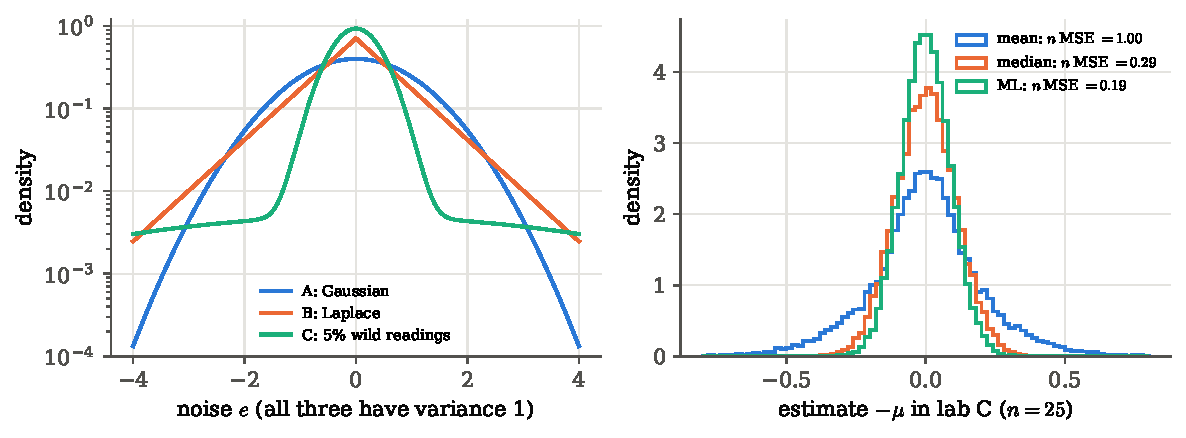
\includegraphics[width=\linewidth]{figures/chT5/three_labs.pdf}
\caption{Left: the noise laws of the three laboratories, all of variance
one, on a logarithmic scale. The Gaussian (A) has the thinnest tails; the
Laplace law (B) falls in straight lines; laboratory C has a narrow core and
a broad skirt made by the 5\% of wild readings. Right: in laboratory C, the
estimates of $\mu$ from $\TFiveALabM$ experiments of $\TFiveALabN$ readings.
The mean (blue) is about twice as wide as the median (orange) and the
maximum-likelihood estimate (green).}
\label{T5a:fig:three-labs}
\end{figure}

\paragraph{A picture: how hard each reading pulls.}
Every estimator in this example can be written as the solution of one
equation. Maximum likelihood sets the slope of the log likelihood to zero,
$\sum_i\psi(x_i-\mu)=0$ with $\psi(e)=-\dd\ln f(e)/\dd e$. Read $\psi(e)$ as
the \emph{pull} that a reading at distance $e$ from the current guess exerts
on the guess; the estimate is where the pulls from above and below balance.
For Gaussian noise $-\ln f=\frac12e^2+\text{const}$, so $\psi(e)=e$: a
reading pulls in proportion to its distance, like a spring. A reading ten
units away pulls ten times as hard as one at one unit, and this is why one
stopped watch can move the average by an hour. For Laplace noise
$\psi(e)=\sgn(e)/b$: every reading pulls equally hard, whatever its
distance, so only the counts above and below matter. For laboratory C the
pull grows like a spring near the centre, then \emph{falls back} for
readings far out, because the mixture law ``knows'' that far readings are
probably cosmic rays and carry little information about $\mu$.
\Cref{T5a:fig:pull} draws the three pulls. Choosing an estimator is choosing
how hard each reading may pull, and the best choice is the one that matches
the law of the noise.

\begin{figure}[htbp]
\centering
\begin{tikzpicture}
\begin{axis}[width=10cm,height=6.4cm,xmin=-6,xmax=6,ymin=-9,ymax=9,
  axis lines=middle,xlabel={$e$},ylabel={pull $\psi(e)$},
  xlabel style={anchor=north west},ylabel style={anchor=south},
  legend style={font=\scriptsize,draw=none,fill=white,at={(0.02,0.98)},anchor=north west},
  tick label style={font=\scriptsize},samples=241,domain=-6:6]
  \addplot[thick,formblue] {x};
  \addlegendentry{A: Gaussian, $\psi=e$}
  \addplot[thick,fibreorange,samples=401] {sign(x)*sqrt(2)};
  \addlegendentry{B: Laplace, $\psi=\sgn(e)/b$}
  \addplot[thick,tangentgreen,samples=481]
    {(0.95*exp(-x^2/(2*0.40996^2))*x/0.40996^3 + 0.05*exp(-x^2/(2*4.0996^2))*x/(4.0996^3))
     /(0.95*exp(-x^2/(2*0.40996^2))/0.40996 + 0.05*exp(-x^2/(2*4.0996^2))/4.0996)};
  \addlegendentry{C: 5\% wild readings}
\end{axis}
\end{tikzpicture}
\caption{The pull $\psi(e)=-\dd\ln f/\dd e$ that a reading at distance $e$
exerts on the estimate, for the three noise laws (all of variance one).
Gaussian noise pulls like a spring, without limit. Laplace noise pulls with
the same strength at every distance. The law of laboratory C pulls hard near
the centre and then lets go: a reading more than about $1.3$ units away is
treated as a probable cosmic ray.}
\label{T5a:fig:pull}
\end{figure}

\paragraph{One idea, many names.}
Choosing a rule that turns data into an answer, by asking how much each
possible error would cost us and which rule keeps the expected cost low, is
called \newterm{statistical decision theory} \mainref{Ch.~12}. The cost is
the \emph{loss}, its average over repeated experiments the \emph{risk}, and
the rule the estimator. The ``balance of pulls'' equation
$\sum_i\psi(x_i-\mu)=0$ is called an \emph{estimating equation}, and
estimators defined by one are \emph{M-estimators}
(\srcref{CasellaBerger}{\S10.2.2, p.~391}): maximum likelihood is the case
$\psi=-(\ln f)'$, least squares the case $\psi(e)=e$, the median the case
$\psi=\sgn$. The same idea gives the matched filter of a gravitational-wave
search (the weights match the noise spectrum, \cref{ch:10}) and the
weighted mean (the weights match each reading's variance,
\cref{3a:sec:blue}). In every case the recipe is tuned to what we know about
how the data go wrong.

What follows turns the three laboratories into a short list of questions,
then places every estimator of the book on one table. The rest of the
chapter builds the families that the earlier chapters did not.

\subsection{Six questions}
\label{T5a:sec:six-questions}

Each question below is asked about the problem, not about the data
already in hand, and each answer points to a family of estimators.
\Cref{T5a:fig:roadmap} at the start of the chapter draws them in order.

\paragraph{(i) What do we know about the noise?} This is the question the
three laboratories answered. If we know its full law, the likelihood is
available and maximum likelihood is efficient for large samples
(\cref{3b:sec:cramer-rao}). If we know only the mean and the covariance of
the noise, as is common when an instrument comes with a noise covariance
matrix but no promise that the noise is Gaussian, the natural recipe is the
best \emph{linear} unbiased estimator of \cref{T5a:sec:blue}, which needs
nothing else. If we know that most readings are well behaved but some may be
wild, we need a \emph{robust} estimator (\cref{T5a:sec:robust}). If we know
only a few moments of the data as functions of the parameter, the method of
moments matches them (\cref{3b:sec:mom}, \srcref{Cowan}{Ch.~8, pp.~114--117}).
In laboratory A all of these coincide with the mean; in laboratory C they
differ by a factor of five.

\paragraph{(ii) Do we have prior information worth using?} If earlier
experiments or physics already tell us roughly where $\mu$ lies, a Bayes
estimator uses it, and its quality depends on whether the prior is right.
Near the prior guess it beats every unbiased estimator; far from it, it is
worse. \Cref{T5a:sec:bayes-risk} computes both sides of this trade, and the
linear--Gaussian case becomes the Wiener filter.

\paragraph{(iii) Where does the parameter live?} In the three laboratories
$\mu$ shifts every reading: it lives in the \emph{mean} of the data, and an
estimator linear in the data can find it. Sometimes the parameter changes
how much the data \emph{scatter}: the amplitude of the sky fluctuations, the
level of a noise, a power spectrum. Then the mean of the data is zero
whatever the parameter, so no linear combination of the readings can see it,
and the estimator must be \emph{quadratic} in the data
(\cref{T5a:sec:quadratic}).

\paragraph{(iv) How many parameters at once?} One number is estimated well
by its own data. When many similar numbers are estimated together, the
calibrations of a hundred detectors, the band powers of a spectrum, each one
can borrow strength from the others, and shrinking all estimates towards a
common value lowers the total error (\cref{T5a:sec:stein}).

\paragraph{(v) Do the data arrive all at once or in a stream?} If readings
keep coming, we would rather update the estimate than recompute it from
scratch. Recursive estimators do this; the second half of the chapter
builds them.

\paragraph{(vi) Does the best estimator depend on what it estimates?} The
best weights for a power spectrum depend on the spectrum; the best weights
for a robust fit depend on which readings are outliers, which depends on the
fit. Such estimators are found by iterating, also in the second half of the
chapter.

\paragraph{Example: three questions for one problem.} A CCD camera takes
$n$ dark frames to measure the dark current of one pixel, the rate $\mu$ at
which it collects charge with the shutter closed. (i) The noise of each frame
is read-out noise plus Poisson noise of the dark charge, nearly Gaussian, but
cosmic rays hit a few per cent of the frames: we are in laboratory C, and a
robust estimator is called for. (ii) The manufacturer quotes a typical dark
current, but it varies from pixel to pixel by more than our measurement
error, so it is a weak prior at best. (iv) We are not measuring one pixel
but four million at once, and they come from the same manufacturing process:
shrinking each pixel's estimate towards the chip-wide average lowers the
total error. The ``best'' estimator for this pixel is therefore a robust
estimate, shrunk towards the chip average. No single textbook recipe gives
it, but each ingredient answers one question.

\subsection{Every estimator in one picture}
\label{T5a:sec:taxonomy}

The estimators met so far, and those of this chapter, differ in three
things: what they \emph{assume} about the data, what they \emph{optimise},
and therefore \emph{when} they are the right tool. \Cref{T5a:tab:taxonomy}
lists them side by side. Reading down the ``assumes'' column shows a
ladder: the more we know about the noise, the more efficient the estimator
that knowledge allows, and the more it costs when the knowledge is wrong.

\begin{taxonomy}[Which estimator assumes what, and optimises what]
\label{T5a:tab:taxonomy}
\small
\begin{tabularx}{\linewidth}{@{}p{24mm}XXp{19mm}@{}}
\toprule
estimator & assumes & optimises / guarantees & where\\
\midrule
method of moments & a few moments as functions of $\theta$ & consistency; simple, often a starting point & \cref{3b:sec:mom}\\
maximum likelihood & the full law of the data & efficient for large $n$ (reaches Cram\'er--Rao) & \cref{3b:sec:mle}\\
least squares & Gaussian noise, or only mean and covariance & ML for Gaussian; BLUE for any noise & \cref{3b:sec:least-squares}\\
weighted mean & independent readings, known variances & minimum variance among weighted averages & \cref{3a:sec:blue}\\
linear (BLUE) & $\data=\mathbf A\params+\bm n$, known $\Cov\bm n$ & minimum variance among linear unbiased & \cref{T5a:sec:blue}\\
minimum-variance unbiased & full law, a complete sufficient statistic & minimum variance among all unbiased & \cref{3b:sec:recipe-best}\\
Bayes (mean, median, mode) & a prior and a loss & lowest average risk over the prior & \cref{3b:sec:recipe-candidates,T5a:sec:bayes-risk}\\
Wiener filter, ridge & Gaussian signal prior and noise & minimum mean squared error & \cref{T5a:sec:wiener}\\
shrinkage (James--Stein) & many similar means, Gaussian noise & total mean squared error below ML for $k\ge3$ & \cref{T5a:sec:stein}\\
robust (M, Huber, median) & most readings well behaved & bounded influence; efficiency near ML & \cref{T5a:sec:robust}\\
quadratic (QML) & $\theta$ in the covariance, Gaussian data & minimum variance unbiased quadratic & \cref{T5a:sec:quadratic}\\
iterative & best estimator needs $\theta$ & converges to the optimum & second half\\
recursive & data in a stream & same answer, updated reading by reading & second half\\
\bottomrule
\end{tabularx}
\end{taxonomy}

Two features of the table are worth saying in words. First, almost every
row ``optimises'' something different, so there is no single best
estimator: there is a best estimator \emph{for a stated criterion under
stated assumptions}. \Cref{3a:sec:mse-theta} already showed that even for
one Gaussian mean no estimator has the lowest mean squared error at every
true value. Second, the rows are not rivals. In laboratory A the weighted
mean, least squares, the BLUE, maximum likelihood and the minimum-variance
unbiased estimator are \emph{one and the same estimator}, the sample mean.
They come apart only when the noise is not Gaussian, when a prior is used,
or when the parameter moves from the mean into the covariance. Those
departures are what the rest of the chapter is about.

\begin{pitfall}[Inefficient is not wrong]
Under the heavy-tailed noise of laboratory C the sample mean is still
unbiased, and its error bar $\sigma/\sqrt n$ is still correct. What it loses
is \emph{efficiency}: it needs about five times as many readings as maximum
likelihood to reach the same precision. A badly chosen estimator rarely
gives a wrong answer; it gives an honest but needlessly large error bar. The
exception is a lopsided contamination, cosmic rays that only ever add
charge, which biases the mean as well (\cref{T5a:sec:robust}).
\end{pitfall}
\section{Linear estimators and the Gauss--Markov theorem}
\label{T5a:sec:blue}

\paragraph{What we already have.}
For readings of one quantity with known variances, \cref{3a:sec:blue} found
the weights that make a weighted average scatter least: each reading is
weighted by its inverse variance. \Cref{3a:sec:weighted-corr} let the
readings be correlated, and \cref{3b:sec:linear-ls} fitted several
parameters at once by least squares and found the covariance of the result,
$(\mathbf A\T\Cmat^{-1}\mathbf A)^{-1}$ (\cref{3b:eq:ls-cov}). Along the way
\cref{3a:sec:weighted-corr} mentioned that these answers are instances of a
theorem named after Gauss and Markov, without proving it.

\paragraph{When that is not enough.}
Two questions were left open. First, least squares was derived as maximum
likelihood for \emph{Gaussian} noise. Is it still a good recipe when the
noise is not Gaussian, or when we do not know its law? Second, with several
parameters and correlated noise, could some other combination of the
readings, one we did not think of, do better? The theorem answers both, and
its proof is short enough to do in full.

\paragraph{A story: three weighings of two letters.}
A kitchen scale has a random error of about a gram. We want the weights of
two letters, so we weigh the first, then the second, and then, almost by
accident, both together. What is our best estimate of the first letter? The
obvious answer is the first weighing. But the third weighing also knows
about the first letter: subtracting the second weighing from it gives a
second, independent estimate. Combining all three readings, with the right
signs and weights, beats the obvious answer. Nothing about the scale's error
needs to be Gaussian for this to work; it only needs to average to zero and
to have a known spread.

The same situation is everywhere in physics. A CMB telescope sweeps across
the sky and each sample of the time stream sees one pixel: the pixel values
are the unknowns, the time stream is the data, and every pixel is seen many
times along different scans, with noise correlated in time. Turning the time
stream into a map is the weighing problem with millions of letters. A
straight-line fit, a calibration of detector gains from single and
coincident hits, a template fit for foregrounds: each is a set of readings
that are \emph{linear} in the unknowns plus noise. The idea of the section
is that for every such problem there is one best linear recipe, and it
depends on the noise only through its covariance.

\paragraph{The story in symbols.}
Call the two weights $m_1,m_2$ and the three readings
$d_1=m_1+n_1$, $d_2=m_2+n_2$, $d_3=m_1+m_2+n_3$, with independent errors of
mean zero and variance $\sigma^2$. In matrix form
\begin{equation}
  \data=\mathbf A\params+\bm n,\qquad
  \data=\begin{pmatrix}d_1\\d_2\\d_3\end{pmatrix},\quad
  \mathbf A=\begin{pmatrix}1&0\\0&1\\1&1\end{pmatrix},\quad
  \params=\begin{pmatrix}m_1\\m_2\end{pmatrix},\quad
  \Cov\bm n=\sigma^2\Id .
  \label{T5a:eq:weighing}
\end{equation}
A linear estimate of $m_1$ is $\hat m_1=w_1d_1+w_2d_2+w_3d_3$, with three
dials. Its mean is
$w_1m_1+w_2m_2+w_3(m_1+m_2)=(w_1+w_3)m_1+(w_2+w_3)m_2$, so it is unbiased for
every pair of weights exactly when $w_1+w_3=1$ and $w_2+w_3=0$. That leaves
one free dial, say $w_3=t$, giving $w_1=1-t$, $w_2=-t$, and variance
\begin{align}
  \Var\hat m_1
  &\eqby{1}\sigma^2\bigl[(1-t)^2+t^2+t^2\bigr]
   \eqby{2}\sigma^2\bigl[1-2t+3t^2\bigr]
   \eqby{3}\sigma^2\Bigl[3\bigl(t-\tfrac13\bigr)^2+\tfrac23\Bigr].
  \label{T5a:eq:weighing-var}
\end{align}
\begin{explain}
  \item Independent errors: the variance of a weighted sum is $\sigma^2\sum_iw_i^2$ (\cref{3a:eq:var-sum}).
  \item Expand $(1-t)^2=1-2t+t^2$ and add.
  \item Complete the square: $3t^2-2t+1=3(t^2-\frac23t+\frac19)+1-\frac13$.
\end{explain}
The naive choice $t=0$ (use $d_1$ alone) gives $\sigma^2$. The choice
$t=1$ (use $d_3-d_2$) gives $2\sigma^2$. The minimum is at $t=\frac13$:
\begin{equation}
  \hat m_1=\tfrac13\,(2d_1-d_2+d_3),\qquad \Var\hat m_1=\tfrac23\,\sigma^2 ,
  \label{T5a:eq:weighing-blue}
\end{equation}
and by symmetry $\hat m_2=\frac13(-d_1+2d_2+d_3)$. The price of the gain is a
correlation: both estimates use $d_3$, and $\Cov(\hat m_1,\hat m_2)
=\frac{\sigma^2}{9}[2\cdot(-1)+(-1)\cdot2+1\cdot1]=-\frac{\sigma^2}{3}$,
a correlation coefficient of $-\frac12$. Lesson: a reading that involves
several unknowns informs all of them, and the best linear recipe uses every
reading, with weights that can be negative.

\paragraph{A picture: the best weights touch the smallest ellipse.}
Strip the problem to two readings of one quantity $\mu$, with variances $1$
and $4$. The weights $(w_1,w_2)$ form a plane. Unbiasedness, $w_1+w_2=1$,
is a straight line in that plane. The variance $w_1^2+4w_2^2$ is constant
on ellipses centred at the origin, twice as long in $w_1$ as in $w_2$.
Moving along the line, we cross ellipses of different sizes; the best
weights are where the line just touches the smallest ellipse it can reach
(\cref{T5a:fig:blue-ellipse}). At that point the line is tangent to the
ellipse, so the ellipse's gradient $(2w_1,8w_2)$ is perpendicular to the line,
that is parallel to $(1,1)$: $2w_1=8w_2$, so $w_1=4w_2$, and with $w_1+w_2=1$
the weights are $(0.8,0.2)$, the inverse-variance weights of
\cref{3a:eq:wmean-weights}. The Gauss--Markov theorem is this picture in any
number of dimensions: a flat set of allowed weights, a family of nested
ellipsoids of equal variance, and one point of contact.

\begin{figure}[htbp]
\centering
\begin{tikzpicture}[scale=3.2]
  \draw[faint,->] (-0.35,0) -- (1.45,0) node[right,black] {$w_1$};
  \draw[faint,->] (0,-0.35) -- (0,1.0) node[above,black] {$w_2$};
  \draw[formblue!45] (0,0) ellipse ({sqrt(0.4)} and {sqrt(0.4)/2});
  \draw[formblue,thick] (0,0) ellipse ({sqrt(0.8)} and {sqrt(0.8)/2});
  \draw[formblue!45,dashed] (0,0) ellipse ({sqrt(1.25)} and {sqrt(1.25)/2});
  \draw[bdry] (-0.25,1.25*0.76) -- (1.35,-0.35);
  \fill[fibreorange] (0.8,0.2) circle (0.025);
  \fill[softgray] (0.5,0.5) circle (0.022);
  \node[lbl,anchor=south west] at (0.82,0.22) {$(0.8,0.2)$: least variance, $0.8$};
  \node[lbl,anchor=south west] at (0.52,0.52) {$(0.5,0.5)$: variance $1.25$};
  \node[lbl,bdryred,anchor=east] at (-0.06,1.0) {$w_1+w_2=1$};
  \node[lbl,formblue,anchor=north] at (0.0,-0.47) {equal-variance ellipses $w_1^2+4w_2^2=c$};
\end{tikzpicture}
\caption{Two readings of one quantity, with variances $1$ and $4$. Every
pair of weights on the red line gives an unbiased average. The blue ellipses
are sets of weights with equal variance ($c=0.4$, $0.8$ and $1.25$, from the
inside out). The smallest ellipse the line reaches touches it at the
inverse-variance weights $(0.8,0.2)$, with variance $0.8$. Equal weights
(grey dot) lie on a larger ellipse, with variance $1.25$.}
\label{T5a:fig:blue-ellipse}
\end{figure}

\paragraph{One idea, many names.}
The best linear recipe goes by many names. Statisticians call it
\newterm{generalised least squares} or the \newterm{best linear unbiased
estimator} (BLUE); in regression it is the least-squares solution
$(\mathbf X\T\mathbf X)^{-1}\mathbf X\T\bm Y$ \mainref{Thm~13.13, p.~217};
CMB experiments call it the map-making equation; the internal linear
combination that cleans the CMB of Galactic dust (\cref{3a:sec:weighted-corr})
is the same formula with one unknown; and the Kalman filter of the second
half of the chapter applies it one reading at a time. Linear algebra is the
natural language because the data, the unknowns and the weights are all
lists of numbers, and ``unbiased'' and ``least variance'' turn into a linear
constraint and a quadratic form.

We first set up the general linear model and prove that one recipe beats
every other linear unbiased one, then ask what it needs from the noise, and
finally what it cannot do when the noise has heavy tails.

\subsection{The linear model and its best linear unbiased estimator}
\label{T5a:sec:blue-proof}

\begin{workdef}[linear model, BLUE]
A \newterm{linear model} writes $N$ readings as
$\data=\mathbf A\params+\bm n$, where $\params$ holds $m$ unknown parameters,
$\mathbf A$ is a known $N\times m$ matrix \unpack{column $j$ says how strongly
parameter $j$ enters each reading} with independent columns, and the noise
$\bm n$ has mean zero and a known, positive-definite covariance $\Cmat$.
A \newterm{linear estimator} is $\hat\params=\mathbf W\data$ for a fixed
$m\times N$ matrix $\mathbf W$. It is unbiased if $\E\hat\params=\params$ for
every $\params$. The \newterm{best linear unbiased estimator} is the
unbiased $\mathbf W$ for which every combination $\bm u\T\hat\params$ has the
smallest possible variance.
\end{workdef}

The noise here needs only two properties, a mean of zero and a known
covariance. No distribution has been assumed.

\emph{What does unbiased require?} The mean of a linear estimator is
\begin{equation}
  \E\hat\params\eqby{1}\mathbf W\,\E\data\eqby{2}\mathbf W\mathbf A\params ,
  \label{T5a:eq:lin-mean}
\end{equation}
\begin{explain}
  \item Expectation is linear and $\mathbf W$ is a fixed matrix.
  \item $\E\data=\mathbf A\params+\E\bm n$ and $\E\bm n=\bm0$.
\end{explain}
and $\mathbf W\mathbf A\params=\params$ for \emph{every} $\params$ means
$\mathbf W\mathbf A=\Id_m$: taking $\params$ to be each unit vector in turn
reads off the columns of $\mathbf W\mathbf A$ one at a time. This is the
matrix version of $w_1+w_3=1$, $w_2+w_3=0$ in the weighing story.

\emph{How much does it scatter?} The covariance of a linear map of the data
is the map applied on both sides (\cref{3a:eq:prop-matrix}):
$\Cov\hat\params=\mathbf W\Cmat\mathbf W\T$.

\emph{A candidate.} Least squares with weight $\Cmat^{-1}$ gave
$\mathbf W_0=(\mathbf A\T\Cmat^{-1}\mathbf A)^{-1}\mathbf A\T\Cmat^{-1}$
(\cref{3b:eq:normal-eq}). It is unbiased, since
$\mathbf W_0\mathbf A=(\mathbf A\T\Cmat^{-1}\mathbf A)^{-1}(\mathbf A\T\Cmat^{-1}\mathbf A)=\Id$,
and its covariance is
\begin{equation}
  \mathbf W_0\Cmat\mathbf W_0\T
  \eqby{1}(\mathbf A\T\Cmat^{-1}\mathbf A)^{-1}\mathbf A\T\Cmat^{-1}\,\Cmat\,\Cmat^{-1}\mathbf A\,(\mathbf A\T\Cmat^{-1}\mathbf A)^{-1}
  \eqby{2}(\mathbf A\T\Cmat^{-1}\mathbf A)^{-1} .
  \label{T5a:eq:blue-cov}
\end{equation}
\begin{explain}
  \item Insert $\mathbf W_0$; its transpose is $\Cmat^{-1}\mathbf A(\mathbf A\T\Cmat^{-1}\mathbf A)^{-1}$ because $\Cmat$ and $\mathbf A\T\Cmat^{-1}\mathbf A$ are symmetric.
  \item $\Cmat^{-1}\Cmat\Cmat^{-1}=\Cmat^{-1}$, then one factor $\mathbf A\T\Cmat^{-1}\mathbf A$ cancels against its inverse.
\end{explain}

\emph{Any other unbiased recipe.} Take any $\mathbf W$ with
$\mathbf W\mathbf A=\Id$ and write it as the candidate plus a difference,
$\mathbf W=\mathbf W_0+\mathbf D$. Both satisfy the constraint, so
$\mathbf D\mathbf A=\mathbf W\mathbf A-\mathbf W_0\mathbf A=\bm0$. Then
\begin{align}
  \mathbf W\Cmat\mathbf W\T
  &\eqby{1}\mathbf W_0\Cmat\mathbf W_0\T+\mathbf W_0\Cmat\mathbf D\T+\mathbf D\Cmat\mathbf W_0\T+\mathbf D\Cmat\mathbf D\T \notag\\
  &\eqby{2}\mathbf W_0\Cmat\mathbf W_0\T+(\mathbf A\T\Cmat^{-1}\mathbf A)^{-1}(\mathbf D\mathbf A)\T+(\mathbf D\mathbf A)(\mathbf A\T\Cmat^{-1}\mathbf A)^{-1}+\mathbf D\Cmat\mathbf D\T \notag\\
  &\eqby{3}(\mathbf A\T\Cmat^{-1}\mathbf A)^{-1}+\mathbf D\Cmat\mathbf D\T .
  \label{T5a:eq:gauss-markov}
\end{align}
\begin{explain}
  \item Multiply out $(\mathbf W_0+\mathbf D)\Cmat(\mathbf W_0+\mathbf D)\T$.
  \item In the cross term, $\mathbf W_0\Cmat=(\mathbf A\T\Cmat^{-1}\mathbf A)^{-1}\mathbf A\T\Cmat^{-1}\Cmat=(\mathbf A\T\Cmat^{-1}\mathbf A)^{-1}\mathbf A\T$, and $\mathbf A\T\mathbf D\T=(\mathbf D\mathbf A)\T$. The other cross term is its transpose.
  \item $\mathbf D\mathbf A=\bm0$ kills both cross terms; the first term is \eqref{T5a:eq:blue-cov}.
\end{explain}
The extra piece $\mathbf D\Cmat\mathbf D\T$ can only add variance. For any
combination $\bm u\T\hat\params$ of the estimates, its contribution is
$\bm u\T\mathbf D\Cmat\mathbf D\T\bm u=\bm v\T\Cmat\bm v$ with
$\bm v=\mathbf D\T\bm u$, and this is non-negative because $\Cmat$ is a
covariance (the variance of the number $\bm v\T\bm n$). It is zero for every
$\bm u$ only if $\mathbf D=\bm0$, since $\Cmat$ is positive definite. So no
linear unbiased recipe can beat $\mathbf W_0$, and only $\mathbf W_0$ itself
can match it.
\begin{keyidea}[Gauss--Markov theorem]
In the linear model $\data=\mathbf A\params+\bm n$ with $\E\bm n=\bm0$ and
$\Cov\bm n=\Cmat$, the estimator
$\hat\params=(\mathbf A\T\Cmat^{-1}\mathbf A)^{-1}\mathbf A\T\Cmat^{-1}\data$
is unbiased, has covariance $(\mathbf A\T\Cmat^{-1}\mathbf A)^{-1}$, and every
other linear unbiased estimator has covariance larger by a positive
semidefinite matrix. It is the unique best linear unbiased estimator,
whatever the law of the noise.
\end{keyidea}

The proof used nothing but $\E\bm n=\bm0$ and $\Cov\bm n=\Cmat$. That is the
content of the remark in \srcref{Cowan}{\S7.2, p.~97} that the least-squares
estimators have zero bias and minimum variance ``regardless of'' the
distributions of the measurements; \srcref{CasellaBerger}{\S11.3.2,
pp.~440--443} proves the one-regressor case and names the theorem.

\paragraph{Example: the weighing design, through the theorem.}
For \eqref{T5a:eq:weighing}, $\mathbf A\T\mathbf A=\begin{pmatrix}2&1\\1&2\end{pmatrix}$,
whose inverse is $\frac13\begin{pmatrix}2&-1\\-1&2\end{pmatrix}$, and with
$\Cmat=\sigma^2\Id$ the factors of $\sigma^2$ cancel in $\mathbf W_0$:
\begin{align}
  \mathbf W_0=(\mathbf A\T\mathbf A)^{-1}\mathbf A\T
  &\eqby{1}\frac13\begin{pmatrix}2&-1\\-1&2\end{pmatrix}\begin{pmatrix}1&0&1\\0&1&1\end{pmatrix}
  \eqby{2}\frac13\begin{pmatrix}2&-1&1\\-1&2&1\end{pmatrix},
  \qquad
  \Cov\hat\params\eqby{3}\frac{\sigma^2}{3}\begin{pmatrix}2&-1\\-1&2\end{pmatrix}.
  \notag
\end{align}
\begin{explain}
  \item $\mathbf A\T$ is the transpose of \eqref{T5a:eq:weighing}.
  \item Row times column: e.g.\ the top-right entry is $2\cdot1+(-1)\cdot1=1$.
  \item \eqref{T5a:eq:blue-cov} with $\Cmat=\sigma^2\Id$: $\sigma^2(\mathbf A\T\mathbf A)^{-1}$.
\end{explain}
The first row is \eqref{T5a:eq:weighing-blue}, now obtained without any
search. The decomposition \eqref{T5a:eq:gauss-markov} also accounts exactly
for the worse recipes. ``Use $d_1$ alone'' is the row $(1,0,0)$, so its
$\mathbf D$-row is $(1,0,0)-\frac13(2,-1,1)=\frac13(1,1,-1)$; it satisfies
$\mathbf D\mathbf A=\bm0$ (check: $\frac13(1+0-1)=0$ and $\frac13(0+1-1)=0$),
and adds $\sigma^2\cdot\frac{1+1+1}{9}=\frac{\sigma^2}{3}$ to the variance,
giving $\frac23\sigma^2+\frac13\sigma^2=\sigma^2$. ``Use $d_3-d_2$'' is
$(0,-1,1)$, its $\mathbf D$-row is $\frac13(-2,-2,2)$, which adds
$\sigma^2\cdot\frac{12}{9}=\frac43\sigma^2$, giving $2\sigma^2$. Both agree
with \eqref{T5a:eq:weighing-var} at $t=0$ and $t=1$. The script
\pyname{code/chT5/02_blue_heavy_tails.py} simulates $\TFiveAWeighM$
weighings with $\sigma=\TFiveAWeighSigma$ and finds variances
$\TFiveAWeighVBlue\,\sigma^2$, $\TFiveAWeighVAlone\,\sigma^2$ and
$\TFiveAWeighVDiff\,\sigma^2$ for the three recipes, and a correlation
$\TFiveAWeighRho$ between $\hat m_1$ and $\hat m_2$.

\paragraph{Example: one quantity, the weighted mean again.}
If all $N$ readings measure the same $\mu$, then $\mathbf A$ is a column of
ones, $\bm1$, and $\params=\mu$. With independent readings,
$\Cmat=\diag(\sigma_1^2,\dots,\sigma_N^2)$, the theorem gives
\begin{equation}
  \hat\mu\eqby{1}\frac{\bm1\T\Cmat^{-1}\data}{\bm1\T\Cmat^{-1}\bm1}
  \eqby{2}\frac{\sum_kd_k/\sigma_k^2}{\sum_k1/\sigma_k^2},
  \qquad
  \Var\hat\mu\eqby{3}\Bigl(\sum_k\frac{1}{\sigma_k^2}\Bigr)^{-1},
  \label{T5a:eq:wmean-again}
\end{equation}
\begin{explain}
  \item $\mathbf A\T\Cmat^{-1}\mathbf A=\bm1\T\Cmat^{-1}\bm1$ is a number, so its inverse is a division.
  \item $\Cmat^{-1}$ is diagonal with entries $1/\sigma_k^2$.
  \item \eqref{T5a:eq:blue-cov}.
\end{explain}
which is the inverse-variance weighted mean of \cref{3a:eq:wmean-weights},
and with a full $\Cmat$ the correlated version \cref{3a:eq:wcorr-weights}.
The Lagrange-multiplier argument of \cref{3a:sec:blue} was the case
$m=1$ of the proof above.

\subsection{What the theorem needs, and what it gives}
\label{T5a:sec:blue-needs}

\emph{For Gaussian noise it is the best estimator of all.} If $\bm n$ is
Gaussian, the BLUE is also the maximum-likelihood estimator
(\cref{3b:sec:ls-from-ml}), and the Fisher matrix of the model is
$\Fish=\mathbf A\T\Cmat^{-1}\mathbf A$: \cref{10a:eq:gauss-fisher} with a mean
$\mathbf A\params$ whose derivative with respect to $\theta_j$ is column $j$
of $\mathbf A$, and a covariance that does not depend on $\params$. So the
BLUE covariance \eqref{T5a:eq:blue-cov} equals $\Fish^{-1}$, the Cram\'er--Rao
bound (\cref{10a:eq:cr-multi}). No unbiased estimator at all, linear or not,
does better: for Gaussian noise the BLUE is the minimum-variance unbiased
estimator.

\emph{For other noise it is the best only among linear recipes.} The
restriction to linear estimators is a real restriction. The median is not a
linear function of the readings (the reading it returns depends on the
order of all of them), so Gauss--Markov says nothing about it, and the three
laboratories of \cref{T5a:sec:questions} showed the median beating the mean,
the BLUE of a common level, by a factor of two or more. Gauss--Markov
guarantees that the BLUE is never \emph{bad} when the covariance is right;
it does not guarantee that it is good.

\emph{It needs the covariance to exist.} For Cauchy noise, such as the
lighthouse flashes of \srcref{Sivia}{\S2.4}, the variance of a single reading
is infinite, so $\Cmat$ does not exist and neither does the BLUE. The mean
of $n$ Cauchy readings has the same Cauchy law as one reading
(\cref{3a:ex:cauchy}), and averaging gains nothing.

\paragraph{Example: the Fisher information of Cauchy noise.}
To see how much better than the median one can do for Cauchy noise, we need
the Cram\'er--Rao bound. With $f(e)=\frac{1}{\pi(1+e^2)}$ and $e=x-\mu$,
\begin{align}
  I
  &\eqby{1}\int_{-\infty}^{\infty}\Bigl(\frac{2e}{1+e^2}\Bigr)^2\frac{\dd e}{\pi(1+e^2)}
   \eqby{2}\frac4\pi\int_{-\pi/2}^{\pi/2}\frac{\tan^2t}{\sec^6t}\,\sec^2t\,\dd t
   \eqby{3}\frac4\pi\int_{-\pi/2}^{\pi/2}\sin^2t\cos^2t\,\dd t \notag\\
  &\eqby{4}\frac4\pi\int_{-\pi/2}^{\pi/2}\frac{\sin^22t}{4}\,\dd t
   \eqby{5}\frac4\pi\cdot\frac{\pi}{8}=\frac12 .
  \label{T5a:eq:cauchy-info}
\end{align}
\begin{explain}
  \item $I=\E[(\partial_\mu\ln f)^2]$, and $\partial_\mu\ln f(x-\mu)=\partial_\mu[-\ln(1+(x-\mu)^2)]=2e/(1+e^2)$.
  \item Substitute $e=\tan t$: $1+e^2=\sec^2t$ and $\dd e=\sec^2t\,\dd t$; $e$ from $-\infty$ to $\infty$ is $t$ from $-\pi/2$ to $\pi/2$.
  \item $\tan^2t/\sec^4t=\sin^2t\cos^2t$.
  \item $\sin t\cos t=\frac12\sin2t$.
  \item $\sin^22t$ averages to $\frac12$ over the interval of length $\pi$, so the integral of $\sin^22t$ is $\pi/2$, and divided by four, $\pi/8$.
\end{explain}
So no unbiased estimator of a Cauchy centre has $n\Var$ below $1/I=2$. The
median reaches $\pi^2/4=\TFiveAHtCauMedTh$ (\cref{3b:sec:efficiency}), so it
wastes about a fifth of the information; maximum likelihood reaches $2$ for
large $n$.

\subsection{When linear is not enough: heavy tails}
\label{T5a:sec:heavy-tails}

How quickly do these large-$n$ statements take hold? We repeat the
comparison of the three laboratories for $n$ from $\TFiveAHtNSmall$ to
$\TFiveAHtNBig$, with $\TFiveAHtM$ experiments at each $n$, for Laplace
noise, Cauchy noise and the contaminated Gaussian of laboratory C. This is
the second part of the script \pyname{02_blue_heavy_tails.py}. The maximum-likelihood estimate is
found by evaluating the log likelihood on a grid of candidate values around
the median and refining the best grid point with a parabola, a direct search
with no iteration.

\pyfile[firstline=66,lastline=72,firstnumber=66]{code/chT5/02_blue_heavy_tails.py}{Mean, median and maximum likelihood for one noise law and one $n$}

Line 68 draws $\TFiveAHtM$ data sets of $n$ readings around $\mu=0$. Line 69
sets the half-width of the grid: wide for small $n$, and wider for the Cauchy
law, whose likelihood can have several peaks. Line 70 finds the
maximum-likelihood estimates, and line 71 records $n$ times the mean squared
error of the three estimators. \Cref{T5a:fig:heavy-tails} shows the result.

\begin{figure}[htbp]
\centering
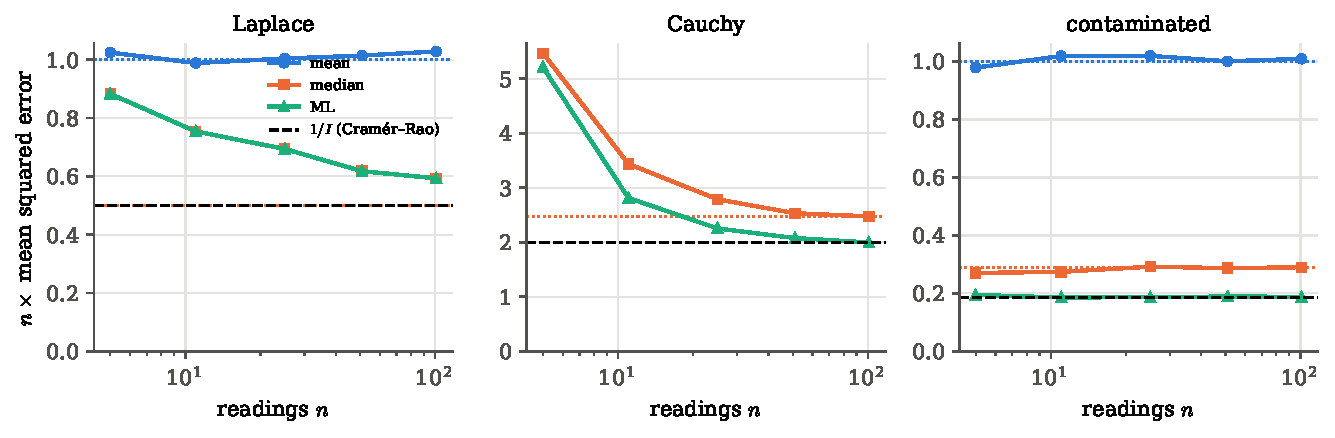
\includegraphics[width=\linewidth]{figures/chT5/heavy_tails.pdf}
\caption{$n$ times the mean squared error of three estimators of a centre,
against the number of readings $n$, for three heavy-tailed noise laws of
unit scale. Dotted lines: the large-$n$ values of the mean (blue, $1$) and
the median (orange, $1/4f(0)^2$). Dashed black: the Cram\'er--Rao value
$1/I$. The mean is absent for Cauchy noise, where its error is infinite.
Maximum likelihood (green) approaches the bound in every case; for Laplace
noise it is the median, and both approach their limit slowly.}
\label{T5a:fig:heavy-tails}
\end{figure}

Three things stand out. For the contaminated Gaussian, every curve is flat
from $n=\TFiveAHtNSmall$ on: the large-$n$ formulas already hold, and maximum
likelihood sits at $\TFiveAHtConML$ against the bound $\TFiveAHtConCR$, five
times better than the mean ($\TFiveAHtConMean$). For Cauchy noise the
small-sample penalty is large: at $n=\TFiveAHtNSmall$ the median and maximum
likelihood have $n\,$MSE $=\TFiveAHtCauMedSmall$ and
$\TFiveAHtCauMLSmall$, and only at $n=\TFiveAHtNBig$ do they reach
$\TFiveAHtCauMed$ and $\TFiveAHtCauML$, close to $\pi^2/4$ and $2$. For
Laplace noise the median (which is maximum likelihood) is still at
$\TFiveAHtLapMed$ for $n=\TFiveAHtNBig$, above the asymptotic $0.5$, and the excess
only roughly halves each time $n$ grows fourfold: the large-$n$ formula is a
statement about a limit, and how soon it applies depends on the noise law. In all
three cases the mean, the BLUE of a common level, is the worst of the three
whenever it exists.

\begin{pitfall}[The BLUE needs the right covariance, not just any covariance]
Gauss--Markov ranks recipes by their variance under the \emph{true}
covariance $\Cmat$. Weights built from a wrong $\Cmat$, for example
correlated noise treated as independent, still give an unbiased estimate,
but its variance is larger than \eqref{T5a:eq:blue-cov}, and the error bar
computed from the wrong $\Cmat$ is wrong as well (\cref{3b:sec:correlated}
shows both effects).
\end{pitfall}

\paragraph{Where this leads.}
Three ways out of the linear world follow from the three laboratories. If
the full law of the noise is known, maximum likelihood uses it
(\cref{3b:sec:mle}). If only ``most readings are well behaved'' is known, a
robust estimator limits the pull of any one reading (\cref{T5a:sec:robust}).
And if we are willing to give up unbiasedness itself, a prior or a shrinkage
rule can lower the mean squared error below anything Gauss--Markov allows,
which is where the next two sections go.
\section{Bayes estimators under repeated experiments}
\label{T5a:sec:bayes-risk}

\paragraph{What we already have.}
A posterior distribution is a whole curve, and to report one number we must
say what kind of mistake we fear. \Cref{3b:sec:recipe-candidates} showed that
the posterior mean minimises the expected squared error, the posterior
median the expected absolute error, and the posterior mode a zero--one loss
(\cref{3b:eq:bayes-squared}, \mainref{Thm~12.8, p.~198}). For Gaussian
readings with a Gaussian prior the posterior mean is a weighted average of
the data's mean and the prior's mean (\cref{5b:eq:normal-post}). Those
statements average over the \emph{parameter}, with the data held fixed at
what we observed.

\paragraph{When that is not enough.}
A colleague who does not share our prior will ask a different question:
``Suppose the true value is $\theta$. If the experiment were repeated many
times, how far would your recipe land from $\theta$, on average?'' That
average is over the \emph{data}, with the parameter held fixed. It is the
question we asked of every estimator in \cref{ch:03}, and a Bayes estimator
can be asked it too. The answer is not ``always better'' or ``always worse'';
it depends on where the truth lies relative to the prior, and knowing how
is what lets us decide whether to use a prior at all.

\paragraph{A story with the whole trick in it.}
Two weather forecasters predict tomorrow's noon temperature. The first
reads only today's sky and instruments, which are noisy. The second does the
same and then pulls the forecast part of the way towards the long-term
average for that day of the year. On ordinary days, which are most days,
the second forecaster is more accurate: the pull cancels part of the noise
in the instruments. On the day of a freak heatwave, the second forecaster is
systematically too cold, because the pull drags the forecast towards a
normal day that tomorrow is not. Whether the pull is worth it depends on how
often the weather is unusual, and by how much.

Physics data behave the same way. A noisy map of the microwave sky, filtered
so that each feature is pulled towards the zero that a prior expects on
small scales, looks cleaner and is closer to the true sky on average, but
every hot spot in it is fainter than it really is. An analysis of a rare
decay that pulls a branching ratio towards the Standard Model value will be
more accurate if the Standard Model is right, and will hide new physics if
it is not.

\paragraph{The story in symbols.}
Let the data reduce to an average $\bar x\sim\Normal(\theta,s^2)$, where $s$
is its standard error, and let the prior be $\theta\sim\Normal(\mu_0,\tau^2)$.
The posterior mean is (\cref{5b:eq:normal-post}, \mainref{Ex.~12.9, p.~198})
\begin{equation}
  \hat\theta_B=w\,\bar x+(1-w)\,\mu_0,\qquad w=\frac{\tau^2}{\tau^2+s^2},
  \label{T5a:eq:bayes-gauss}
\end{equation}
a pull of the data towards $\mu_0$ that is strong when the prior is narrow
($\tau\ll s$) and weak when it is broad. The dial is $\tau$, and the truth
$\theta$ is the unknown that decides whether the dial helps. For a fixed
$\theta$, $\bar x$ varies from experiment to experiment and $\mu_0$ does not,
so
\begin{align}
  \E_\theta\hat\theta_B-\theta
  &\eqby{1}w\theta+(1-w)\mu_0-\theta=(1-w)(\mu_0-\theta), \notag\\
  \Var_\theta\hat\theta_B
  &\eqby{2}w^2s^2, \notag\\
  R(\theta)\equiv\E_\theta(\hat\theta_B-\theta)^2
  &\eqby{3}w^2s^2+(1-w)^2(\theta-\mu_0)^2 .
  \label{T5a:eq:bayes-risk-gauss}
\end{align}
\begin{explain}
  \item $\E_\theta\bar x=\theta$, and the expectation is linear.
  \item Only $\bar x$ varies, with variance $s^2$, and it is multiplied by $w$.
  \item Mean squared error is variance plus squared bias (\cref{3a:eq:mse-decomp}).
\end{explain}
The plain average $\bar x$ has $R=s^2$ for every $\theta$. The Bayes
estimator does better exactly when
\begin{align}
  w^2s^2+(1-w)^2(\theta-\mu_0)^2<s^2
  &\iff (1-w)^2(\theta-\mu_0)^2<(1-w^2)s^2 \notag\\
  &\iff (\theta-\mu_0)^2<\frac{1+w}{1-w}\,s^2
  \iff (\theta-\mu_0)^2<2\tau^2+s^2 ,
  \label{T5a:eq:bayes-cross}
\end{align}
since $1-w^2=(1-w)(1+w)$ and, from \eqref{T5a:eq:bayes-gauss},
$(1+w)/(1-w)=(2\tau^2+s^2)/s^2$. So the pull helps whenever the truth lies
within $\sqrt{2\tau^2+s^2}$ of the prior's centre. For $\tau=s$, $w=\frac12$:
at $\theta=\mu_0$ the error is $s^2/4$, four times smaller than the plain
average's, and the advantage lasts out to
$|\theta-\mu_0|=\sqrt3\,s=\TFiveABrCrossTauOne\,s$. Beyond that the squared
bias grows without limit. Lesson: a prior buys accuracy where it is right
and costs accuracy where it is wrong, and \eqref{T5a:eq:bayes-cross} says
exactly where the boundary is.

\paragraph{A picture: the risk curve.}
Plotting the error $R(\theta)$ against the truth $\theta$ gives the
\newterm{risk curve} of an estimator, its report card for every possible
state of nature. The left panel of \cref{T5a:fig:bayes-risk} shows the flat
line of $\bar x$ and the parabolas \eqref{T5a:eq:bayes-risk-gauss} for three
prior widths. A narrow prior digs a deep valley at $\mu_0$ and climbs
steeply away from it; a broad prior makes a shallow valley and stays close
to the flat line. No curve lies below the flat line everywhere. Choosing an
estimator means choosing which part of the $\theta$ axis to be good at.

\paragraph{One idea, many names.}
Pulling an estimate towards a preferred value to lower its scatter, at the
price of a bias, is called \emph{regularisation} in inverse problems
(\cref{6b:sec:unf-tikhonov} used it to unfold a detector response),
\emph{ridge regression} in statistics and machine learning, the \emph{Wiener
filter} in signal processing and cosmology, and \emph{shrinkage} when many
estimates are pulled together (\cref{T5a:sec:stein}). Asking how a Bayes
estimator behaves over repeated data is the subject of \newterm{statistical
decision theory} \mainref{Ch.~12}, which gives the vocabulary below.

We first define the averages that make ``better'' precise, then work the
binomial example where one estimator is best in the worst case, and then
derive the Wiener filter, the Bayes estimator of a whole signal.

\subsection{Two averages and the Bayes risk}
\label{T5a:sec:two-averages}

\begin{workdef}[loss, risk, Bayes risk, minimax, admissible]
A \newterm{loss} $L(\theta,\hat\theta)$ is the cost of reporting $\hat\theta$
when the truth is $\theta$, e.g.\ $(\hat\theta-\theta)^2$. The
\newterm{risk} is its average over repeated data at fixed truth,
$R(\theta,\hat\theta)=\E_\theta L(\theta,\hat\theta(X))$; for squared loss it
is the mean squared error \mainref{Def.~12.1, p.~194}. The \newterm{Bayes risk}
averages the risk over a prior, $r(\pi,\hat\theta)=\int R(\theta,\hat\theta)\pi(\theta)\,\dd\theta$.
An estimator is \newterm{minimax} if its largest risk,
$\sup_\theta R(\theta,\hat\theta)$, is the smallest possible, and
\newterm{admissible} if no other estimator has a risk at least as low for
every $\theta$ and strictly lower for some \unpack{nobody beats it
everywhere} \mainref{Def.~12.4, 12.17}.
\end{workdef}

The Bayes risk averages twice: over the data at fixed $\theta$, then over
$\theta$. Doing the two integrals in the other order explains why the
posterior mean is the estimator with the smallest Bayes risk
\mainref{Thm~12.7, p.~197}:
\begin{align}
  r(\pi,\hat\theta)
  &\eqby{1}\int\!\!\int L(\theta,\hat\theta(x))\,p(x\given\theta)\,\pi(\theta)\,\dd x\,\dd\theta
   \eqby{2}\int\Bigl[\int L(\theta,\hat\theta(x))\,p(\theta\given x)\,\dd\theta\Bigr]p(x)\,\dd x .
  \label{T5a:eq:bayes-risk-swap}
\end{align}
\begin{explain}
  \item The risk is the integral of the loss against the sampling density $p(x\given\theta)$; then average over $\pi(\theta)$.
  \item Bayes' theorem $p(x\given\theta)\pi(\theta)=p(\theta\given x)p(x)$ (\cref{3b:eq:bayes}), and swap the order of integration.
\end{explain}
The bracket is the posterior expected loss at the observed $x$, and
$p(x)\ge0$. Choosing $\hat\theta(x)$ to make the bracket as small as possible
for every $x$ makes the whole integral as small as possible; for squared loss
that choice is the posterior mean (\cref{3b:eq:bayes-squared}). So the two
viewpoints agree on average: averaged over the prior, nothing beats the
posterior mean. They disagree point by point, as the risk curves show.

\paragraph{Example: the Bayes risk of the Gaussian pull.}
Average \eqref{T5a:eq:bayes-risk-gauss} over the prior, under which
$\E(\theta-\mu_0)^2=\tau^2$:
\begin{equation}
  r\eqby{1}w^2s^2+(1-w)^2\tau^2
  \eqby{2}\frac{\tau^4s^2+s^4\tau^2}{(\tau^2+s^2)^2}
  \eqby{3}\frac{s^2\tau^2}{\tau^2+s^2}=w\,s^2 .
  \label{T5a:eq:bayes-risk-avg}
\end{equation}
\begin{explain}
  \item Linearity: only the bias term depends on $\theta$.
  \item $w=\tau^2/(\tau^2+s^2)$ and $1-w=s^2/(\tau^2+s^2)$.
  \item Factor $s^2\tau^2(\tau^2+s^2)$ out of the numerator.
\end{explain}
Averaged over the prior, the Bayes estimator's error is $w\,s^2$, smaller
than the $s^2$ of $\bar x$ by the factor $w<1$. The gain is large when the
prior is narrow compared with the data's error, and disappears as
$\tau\to\infty$. It is also exactly the posterior variance of
\cref{5b:eq:normal-post}, $1/(1/s^2+1/\tau^2)$: when the prior is the true
distribution of $\theta$, the average error of the posterior mean is the
posterior's own width.

\begin{figure}[htbp]
\centering
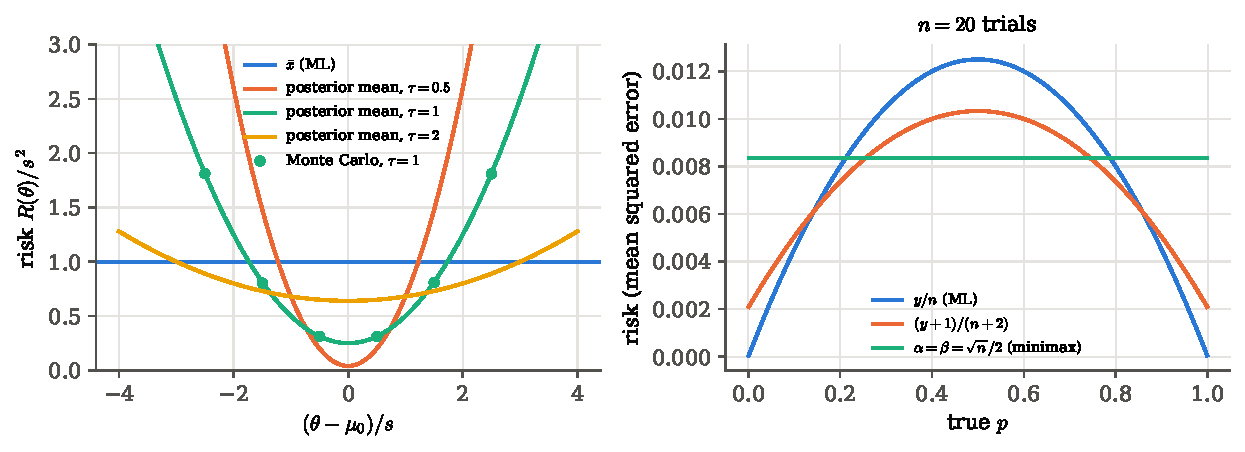
\includegraphics[width=\linewidth]{figures/chT5/bayes_risk.pdf}
\caption{Risk curves. Left: an average $\bar x\sim\Normal(\theta,s^2)$ (flat
blue line) against the posterior mean with a Gaussian prior centred at
$\mu_0$, for three prior widths $\tau$; dots are Monte Carlo estimates
($\TFiveABrM$ experiments each) for $\tau=s$. Each curve dips below the flat
line only within $\sqrt{2\tau^2+s^2}$ of the prior's centre. Right: three
estimators of a probability $p$ from $n=\TFiveABinN$ trials. The
maximum-likelihood $y/n$ is best near $p=0$ and $p=1$, the minimax estimator
(flat green line) is best near $p=\frac12$, and the uniform-prior posterior
mean lies in between.}
\label{T5a:fig:bayes-risk}
\end{figure}

\subsection{Example: the best worst case for a success probability}
\label{T5a:sec:minimax}

A detector registers $y$ hits in $n$ trials, each a hit with probability
$p$. The maximum-likelihood estimate is $y/n$, unbiased with risk
$R=p(1-p)/n$ (\cref{3a:ex:bernoulli}). A Beta$(\alpha,\beta)$ prior gives
the posterior mean $\hat p=(y+\alpha)/(n+\alpha+\beta)$ (\cref{5b:eq:beta-mean}).
Its risk, using $\E y=np$ and $\Var y=np(1-p)$, is \mainref{Ex.~12.3, pp.~194--195}
\begin{align}
  R(p)
  &\eqby{1}\frac{\Var y}{(n+\alpha+\beta)^2}+\Bigl(\frac{np+\alpha}{n+\alpha+\beta}-p\Bigr)^2
   \eqby{2}\frac{np(1-p)+\bigl(\alpha-(\alpha+\beta)p\bigr)^2}{(n+\alpha+\beta)^2}.
  \label{T5a:eq:binom-risk}
\end{align}
\begin{explain}
  \item Variance plus squared bias; the shift by $\alpha$ does not change the variance.
  \item Put the bias over the common denominator: $np+\alpha-(n+\alpha+\beta)p=\alpha-(\alpha+\beta)p$.
\end{explain}
Can the prior be chosen so that the risk does not depend on $p$ at all? Take
$\alpha=\beta=a$ and expand the numerator:
$np-np^2+a^2(1-2p)^2=np-np^2+a^2-4a^2p+4a^2p^2$. The terms in $p$ and $p^2$
cancel when $4a^2=n$, that is $a=\sqrt n/2$, and then the numerator is
$n/4$ for every $p$:
\begin{equation}
  R(p)=\frac{n/4}{(n+\sqrt n)^2}=\frac{1}{4(1+\sqrt n)^2}\qquad\text{for all }p .
  \label{T5a:eq:minimax-binom}
\end{equation}
For $n=\TFiveABinN$ this constant is $\TFiveABinMinimaxRisk$, while the risk
of $y/n$ reaches $1/(4n)=\TFiveABinMLEMax$ at $p=\frac12$. A Bayes estimator
with constant risk is minimax \mainref{Thm~12.11, p.~199}, and the reason is
one line: its Bayes risk is the constant itself, so another estimator with a
lower maximum risk would also have a lower Bayes risk, which the Bayes
estimator does not allow. The right panel of \cref{T5a:fig:bayes-risk} shows
the price: near $p=0$ or $p=1$, where hits are rare or near-certain, the
minimax estimator is much worse than $y/n$, because the prior
Beta$(\TFiveABinAlpha,\TFiveABinAlpha)$ drags it towards $\frac12$. A
physicist measuring a trigger efficiency of $99\%$ would not want it. The
minimax criterion protects the worst case, and here the worst case is not
where we expect to be.

For the Gaussian mean the same logic gives the opposite verdict about the
plain average: $\bar x$ has constant risk $s^2$, and it is the limit of the
posterior means \eqref{T5a:eq:bayes-gauss} as $\tau\to\infty$; it is minimax
and, for a single mean, admissible \mainref{Thm~12.14, 12.20, pp.~200--203}.
No estimator of one Gaussian mean beats $\bar x$ everywhere.
\Cref{T5a:sec:stein} shows that this stops being true as soon as three or
more means are estimated together.

\subsection{The linear--Gaussian case: the Wiener filter and ridge regression}
\label{T5a:sec:wiener}

Now let the unknown be a whole signal: a vector $\bm s$ of pixel values,
Fourier modes or regression coefficients. The data are linear in it,
$\data=\mathbf A\bm s+\bm n$, as in the linear model of \cref{T5a:sec:blue},
with Gaussian noise of covariance $\mathbf N$. The prior says the signal is
itself a Gaussian random vector of mean zero and covariance $\mathbf S$, as a
Gaussian random field is (\cref{ch:07}). The question is the one of
\eqref{T5a:eq:bayes-gauss}, for many numbers at once: what is the posterior
mean of $\bm s$, and how does it behave over repeated data?

\emph{The posterior.} Up to factors that do not depend on $\bm s$, the
posterior is likelihood times prior,
\begin{align}
  -2\ln p(\bm s\given\data)
  &\eqby{1}(\data-\mathbf A\bm s)\T\mathbf N^{-1}(\data-\mathbf A\bm s)+\bm s\T\mathbf S^{-1}\bm s+\text{const} \notag\\
  &\eqby{2}\bm s\T(\mathbf S^{-1}+\mathbf A\T\mathbf N^{-1}\mathbf A)\bm s-2\bm s\T\mathbf A\T\mathbf N^{-1}\data+\text{const} \notag\\
  &\eqby{3}(\bm s-\hat{\bm s})\T\mathbf P(\bm s-\hat{\bm s})+\text{const},
  \qquad \mathbf P=\mathbf S^{-1}+\mathbf A\T\mathbf N^{-1}\mathbf A,\quad
  \mathbf P\hat{\bm s}=\mathbf A\T\mathbf N^{-1}\data .
  \label{T5a:eq:wiener-square}
\end{align}
\begin{explain}
  \item Gaussian likelihood (\cref{3b:eq:like-corr}) and Gaussian prior; normalisations are constants.
  \item Expand the first quadratic form; $\data\T\mathbf N^{-1}\data$ is a constant, and the two cross terms are equal numbers.
  \item Complete the square: expanding the last line gives $\bm s\T\mathbf P\bm s-2\bm s\T\mathbf P\hat{\bm s}+\text{const}$, which matches line two when $\mathbf P\hat{\bm s}=\mathbf A\T\mathbf N^{-1}\data$.
\end{explain}
So the posterior is Gaussian with mean $\hat{\bm s}$ and covariance
$\mathbf P^{-1}$, and the posterior mean, also its mode and median, is
\begin{equation}
  \hat{\bm s}=(\mathbf S^{-1}+\mathbf A\T\mathbf N^{-1}\mathbf A)^{-1}\mathbf A\T\mathbf N^{-1}\data
  =\mathbf S\mathbf A\T(\mathbf A\mathbf S\mathbf A\T+\mathbf N)^{-1}\data .
  \label{T5a:eq:wiener}
\end{equation}
The second form follows from a ``push-through'' identity, checked by
multiplying out:
$\mathbf A\T\mathbf N^{-1}(\mathbf A\mathbf S\mathbf A\T+\mathbf N)
=\mathbf A\T\mathbf N^{-1}\mathbf A\mathbf S\mathbf A\T+\mathbf A\T
=(\mathbf A\T\mathbf N^{-1}\mathbf A+\mathbf S^{-1})\mathbf S\mathbf A\T$;
multiply on the left by $\mathbf P^{-1}$ and on the right by
$(\mathbf A\mathbf S\mathbf A\T+\mathbf N)^{-1}$. The first form inverts a
matrix the size of the signal, the second one the size of the data, and in
practice one uses whichever is smaller. This is the \newterm{Wiener filter}
\srcref{HobsonBMC}{(6.23), p.~141; (10.20), p.~236}.

\emph{Compare it with the BLUE.} Without the prior ($\mathbf S^{-1}\to\bm0$,
an infinitely broad prior) the first form of \eqref{T5a:eq:wiener} becomes
$(\mathbf A\T\mathbf N^{-1}\mathbf A)^{-1}\mathbf A\T\mathbf N^{-1}\data$, the
Gauss--Markov estimator. The prior adds $\mathbf S^{-1}$ to the information
matrix, just as a Gaussian prior adds its precision to a Fisher matrix
(\cref{10a:eq:add}). The price is a bias: for fixed $\bm s$,
$\E\hat{\bm s}=\mathbf P^{-1}\mathbf A\T\mathbf N^{-1}\mathbf A\,\bm s\ne\bm s$.

\paragraph{Example: denoising a stationary signal, one Fourier mode at a time.}
Take $\mathbf A=\Id$, a signal and a noise that are both stationary on a
periodic grid. Both covariances are then diagonal in Fourier space, with
the power spectra $P_s(k)$ and $P_n(k)$ on the diagonal (the Wiener--Khinchin
theorem, \cref{7a:eq:wk}), so \eqref{T5a:eq:wiener} acts on each Fourier mode
separately, as the scalar case \eqref{T5a:eq:bayes-gauss} with $\mu_0=0$:
\begin{equation}
  \hat s_k=w_k\,d_k,\qquad w_k=\frac{P_s(k)}{P_s(k)+P_n(k)} .
  \label{T5a:eq:wiener-fourier}
\end{equation}
Modes where the signal dominates pass almost untouched ($w_k\to1$); modes
where the noise dominates are suppressed ($w_k\to0$). The error and the bias
per mode follow from \eqref{T5a:eq:bayes-risk-gauss} with $s^2\to P_n$ and
$\tau^2\to P_s$:
\begin{align}
  \E|\hat s_k-s_k|^2
  &\eqby{1}(1-w_k)^2P_s+w_k^2P_n
   \eqby{2}\frac{P_n^2P_s+P_s^2P_n}{(P_s+P_n)^2}
   =\frac{P_sP_n}{P_s+P_n}, \notag\\
  \E|\hat s_k|^2
  &\eqby{3}w_k^2(P_s+P_n)=\frac{P_s^2}{P_s+P_n}<P_s .
  \label{T5a:eq:wiener-error}
\end{align}
\begin{explain}
  \item $\hat s_k-s_k=(w_k-1)s_k+w_kn_k$ with independent $s_k$ and $n_k$; average over both, as in the Bayes risk \eqref{T5a:eq:bayes-risk-avg}.
  \item $1-w_k=P_n/(P_s+P_n)$; then factor $P_sP_n(P_s+P_n)$ out of the numerator.
  \item The data mode $d_k=s_k+n_k$ has power $P_s+P_n$, multiplied by $w_k^2$.
\end{explain}
The error per mode is smaller than both $P_n$ (the raw data) and $P_s$ (the
prior guess $\hat s=0$), so the Wiener filter beats both. But the filtered
signal has \emph{less} power than the true one: every feature is fainter, the
``oversmoothing'' of \srcref{HobsonBMC}{p.~237}.

The script \pyname{code/chT5/03_bayes_risk.py} draws $\TFiveAWfM$ periodic
signals of $\TFiveAWfNpix$ pixels with a smooth spectrum that equals the white
noise level at $k\approx\TFiveAWfKcross$, adds the noise, and filters with
\eqref{T5a:eq:wiener-fourier}. The mean squared error per pixel drops from
$\TFiveAWfMseRaw$ in the raw data to $\TFiveAWfMse$ after filtering
(prediction $\TFiveAWfMseTh$). The variance of the filtered map is
$\TFiveAWfVarRec$ (prediction $\TFiveAWfVarRecTh$), against $\TFiveAWfVarSig$
for the true signal: the filtered map is ten times closer to the truth and
visibly fainter (\cref{T5a:fig:wiener}). The script also checks that the two
matrix forms in \eqref{T5a:eq:wiener} and the Fourier form agree on a small
grid.

\begin{figure}[htbp]
\centering
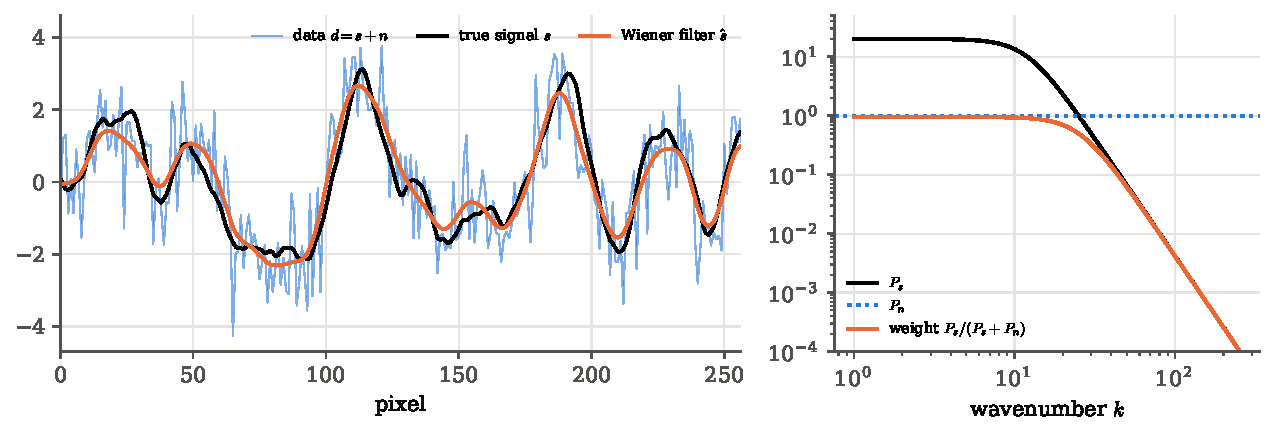
\includegraphics[width=\linewidth]{figures/chT5/wiener.pdf}
\caption{Left: one realisation of a smooth periodic signal (black), the
signal plus white noise (light blue), and the Wiener-filtered estimate
(orange). The filter removes most of the noise but also flattens the peaks.
Right: the signal and noise power spectra and the filter weight
$P_s/(P_s+P_n)$, which is close to one where the signal dominates and falls
like $P_s/P_n$ where the noise does.}
\label{T5a:fig:wiener}
\end{figure}

\paragraph{Example: ridge regression is a Wiener filter.}
Fit $m$ coefficients $\params$ to $N$ readings with independent noise of
variance $\sigma^2$, $\data=\mathbf A\params+\bm n$, and put an independent
Gaussian prior of width $\tau$ on each coefficient: $\mathbf N=\sigma^2\Id$,
$\mathbf S=\tau^2\Id$. The first form of \eqref{T5a:eq:wiener} becomes
\begin{equation}
  \hat\params
  \eqby{1}\Bigl(\frac{\Id}{\tau^2}+\frac{\mathbf A\T\mathbf A}{\sigma^2}\Bigr)^{-1}\frac{\mathbf A\T\data}{\sigma^2}
  \eqby{2}(\mathbf A\T\mathbf A+\lambda\Id)^{-1}\mathbf A\T\data,
  \qquad\lambda=\frac{\sigma^2}{\tau^2},
  \label{T5a:eq:ridge}
\end{equation}
\begin{explain}
  \item Insert $\mathbf S^{-1}=\Id/\tau^2$ and $\mathbf N^{-1}=\Id/\sigma^2$.
  \item Multiply the bracket by $\sigma^2$ and its inverse by $1/\sigma^2$; the factors cancel against the $1/\sigma^2$ on the right.
\end{explain}
the \newterm{ridge regression} estimator. Without the $\lambda\Id$ it is
ordinary least squares; adding $\lambda$ to the diagonal of $\mathbf A\T\mathbf A$
keeps the inverse well behaved when the columns of $\mathbf A$ are nearly
dependent (a polynomial of high degree, an unfolding matrix), which is
exactly where least squares has enormous variance. The Tikhonov unfolding of
\cref{6b:eq:unf-tik} is the same estimator with a curvature penalty in place
of $\lambda\Id$, and its MSE-optimal filter factor \cref{6b:eq:unf-wiener} is
\eqref{T5a:eq:wiener-fourier} once more. In the map-to-map comparison of
\cref{12w:eq:pearson} the weight $C/(C+N)$ that maximises the correlation
with the true map is the same filter again.

\begin{pitfall}[A Wiener-filtered map has the wrong power spectrum]
By \eqref{T5a:eq:wiener-error}, the power of a Wiener-filtered map is
$P_s^2/(P_s+P_n)$, not $P_s$. Measuring a power spectrum, or counting hot
spots, or computing any statistic of the field on the filtered map gives a
biased answer unless the filter is undone in the statistic. The filtered map
is the best map in the mean-squared sense; it is not a typical realisation
of the sky.
\end{pitfall}

\paragraph{When to use a Bayes estimator.}
Three situations favour it. When the prior is genuinely known, as for a
population of objects whose distribution we have measured before, or a
Gaussian random field whose spectrum is known, the Bayes estimator has the
smallest average error, and nothing else should be used. When the data alone
are nearly degenerate, as in an unfolding or a fit with many coefficients,
a mild prior turns an unusable estimate into a usable one, at a bias we can
compute. When the goal is a map or a reconstruction to look at, the Wiener
filter is the natural choice. In the opposite situation, a single parameter
where an unexpected value is the discovery we hope for, a prior that pulls
towards the expected value is the wrong tool: an unbiased estimate with an
honest error bar, and a likelihood that others can combine with their own
priors, serves better.
\section{Many parameters at once: shrinkage and Stein's paradox}
\label{T5a:sec:stein}

\paragraph{What we already have.}
For one Gaussian mean, \cref{T5a:sec:minimax} recalled that the plain average
cannot be beaten everywhere: any estimator better than it for some true
values is worse for others. \Cref{3a:ex:shrinkage} showed the simplest such
trade, $c\bar x$ with $c<1$, which wins near zero and loses far from it, and
\cref{T5a:sec:bayes-risk} showed that a prior turns this pull into the
posterior mean. In every case the pull had to be paid for with a known prior
or a lucky truth.

\paragraph{When that is not enough.}
Often we estimate not one number but many of the same kind: the dark
currents of the four million pixels of a CCD (the example at the end of
\cref{T5a:sec:six-questions}), the calibration gains of a hundred detectors,
the band powers of a spectrum, the luminosities of a sample of galaxies.
Each has its own data, and estimating each by its own average looks like
the obvious and even the only fair thing to do. Surprisingly, when there are
three or more of them, it is not the best thing to do, even with no prior at
all.

\paragraph{A story with the whole trick in it.}
Early in a baseball season, a few players have batted spectacularly well
and a few spectacularly badly, over only a few dozen attempts each. Who will
have the best average at the end of the season? Experience says: the stars
of April will still be good, but not as good as in April, and the April
failures will recover somewhat. Part of an extreme early record is luck,
and luck does not repeat. So the best forecast for every player pulls his
early average part of the way towards the average of all players. The pull
is not a prior opinion about any player: its size is learned from the
spread of all the early records together. Efron and Morris used exactly
this example to make the idea famous \cite{EfronMorris1975,EfronMorris1977}.

The physics is the same. Among a hundred detector gains measured with equal
noise, the ones that came out highest are, on average, the ones whose noise
happened to be positive. Pulling all the estimates towards their common
average undoes part of that selection and lowers the total error. The idea
of the section is that estimating many similar numbers together, and
letting them borrow strength from each other, beats estimating each on its
own.

\paragraph{The story in symbols.}
Take $k$ readings $X_i\sim\Normal(\theta_i,1)$, $i=1,\dots,k$, independent,
one per unknown mean, and judge an estimator by its total squared error
$\sum_i(\hat\theta_i-\theta_i)^2$. Write $\bm X=(X_1,\dots,X_k)$ and
$\params=(\theta_1,\dots,\theta_k)$. Maximum likelihood takes
$\hat\params=\bm X$, with total risk $\sum_i\Var X_i=k$ for every $\params$.
The \newterm{James--Stein estimator} \cite{JamesStein1961} pulls the whole
vector towards the origin by a factor that depends on its length:
\begin{equation}
  \hat\params_{\mathrm{JS}}=\Bigl(1-\frac{c}{|\bm X|^2}\Bigr)\bm X,
  \qquad c=k-2,\qquad |\bm X|^2=\sum_iX_i^2 .
  \label{T5a:eq:james-stein}
\end{equation}
The dial is $c$; $c=0$ is maximum likelihood. The next subsection derives
the total risk for any $c$,
\begin{equation}
  R(\params)=k-\bigl[2c(k-2)-c^2\bigr]\,\E_{\params}\frac{1}{|\bm X|^2},
  \label{T5a:eq:js-risk-c}
\end{equation}
which is below $k$ for every $\params$ whenever $0<c<2(k-2)$, and lowest for
$c=k-2$. The size of the gain: with $k=10$ means that are all zero, the
James--Stein total risk is $2$ instead of $10$. The price: the estimates are
biased towards the origin, and one mean that differs a lot from the others
can be estimated worse than by its own reading. Lesson: for three or more
means, the plain readings are \emph{inadmissible}, beaten everywhere by a
rule that shrinks them together \cite{Stein1956}, \mainref{\S12.7, p.~204}.

\paragraph{A picture: the readings are too far from the origin.}
Why should pulling towards an arbitrary point help? Look at lengths. The
reading is $\bm X=\params+\bm n$, with noise $\bm n$ of mean zero and
$\E|\bm n|^2=k$. On average
$\E|\bm X|^2=|\params|^2+2\params\cdot\E\bm n+\E|\bm n|^2=|\params|^2+k$:
the reading is systematically \emph{longer} than the truth. In many
dimensions the noise vector is almost always nearly perpendicular to
$\params$ (there are $k-1$ directions perpendicular to $\params$ and only
one along it), so $\bm X$ sits on the far side of a right angle, as in
\cref{T5a:fig:js-geometry}, and the point of the line from the origin to
$\bm X$ that is closest to $\params$ lies \emph{inside} $\bm X$. Shrinking
towards the origin moves along that line towards the truth. The amount of
shrinkage needed is about $k/|\bm X|^2$, the excess length squared relative
to the total, and \eqref{T5a:eq:james-stein} estimates it from $|\bm X|^2$
alone. In one or two dimensions the noise is as often along $\params$ as
across it, the picture fails, and so does the gain.

\begin{figure}[htbp]
\centering
\begin{tikzpicture}[scale=1.25]
  \coordinate (O) at (0,0);
  \coordinate (T) at (3,1);
  \coordinate (X) at (2.494,2.518);
  \coordinate (S) at (1.985,2.004);   %
  \draw[faint,dashed] (T) circle (1.6);
  \draw[thick,formblue,->] (O) -- (T);
  \draw[thick,fibreorange,->] (T) -- (X);
  \draw[thick,softgray] (O) -- (X);
  \draw[thick,tangentgreen,->] (X) -- (S);
  \draw[bdryred,dashed] (T) -- (S);
  \draw[faint] ($(T)!0.18cm!(O)$) -- ($($(T)!0.18cm!(O)$)!0.18cm!90:(O)$) -- ($(T)!0.18cm!(X)$);
  \fill (O) circle (0.04); \fill[formblue] (T) circle (0.04);
  \fill[fibreorange] (X) circle (0.04); \fill[tangentgreen] (S) circle (0.04);
  \node[lbl,anchor=north east] at (O) {origin};
  \node[lbl,formblue,anchor=west] at ($(T)+(0.08,-0.05)$) {truth $\params$};
  \node[lbl,fibreorange,anchor=south west] at (X) {reading $\bm X=\params+\bm n$};
  \node[lbl,tangentgreen,anchor=east] at ($(S)+(-0.1,0.05)$) {shrunk};
  \node[lbl,fibreorange,anchor=west] at (3.0,2.0) {$\bm n\perp\params$};
  \node[lbl,align=left,anchor=north west] at (3.9,0.6) {$|\bm X|^2=|\params|^2+|\bm n|^2$\\[1pt] dashed circle: typical noise};
\end{tikzpicture}
\caption{Why shrinkage helps in many dimensions. The noise $\bm n$ is
nearly perpendicular to the truth $\params$, so the reading $\bm X$ is longer
than $\params$ (Pythagoras). Moving from $\bm X$ along the line towards the
origin (green) reaches a point closer to $\params$ than $\bm X$ is: here the
distance drops from $1.6$ to $1.43$. The red dashed segment is the shortest
distance from $\params$ to that line.}
\label{T5a:fig:js-geometry}
\end{figure}

\paragraph{One idea, many names.}
Pulling many estimates towards a common value, with the strength of the pull
learned from the estimates themselves, is called \emph{shrinkage},
\emph{partial pooling} or \emph{borrowing strength}. In Bayesian language it
is a \emph{hierarchical} or \emph{multilevel} model: each $\theta_i$ is drawn
from a population whose spread is itself estimated
\srcref{HobsonBMC}{(11.10), p.~254}, \srcref{Kruschke}{\S9.3}. When the
population spread is estimated by a simple formula and plugged in, the
method is \newterm{empirical Bayes} \cite{EfronMorris1973}. The everyday name
for the effect it corrects is \emph{regression to the mean}.

We now prove \eqref{T5a:eq:js-risk-c} with one identity, read the estimator
as empirical Bayes, check it by simulation, and then say when it should not
be used.

\subsection{Stein's lemma and the James--Stein risk}
\label{T5a:sec:stein-lemma}

The whole proof rests on one identity for a Gaussian variable. Let
$Z\sim\Normal(\theta,1)$ with density $\varphi(z-\theta)$,
$\varphi(u)=e^{-u^2/2}/\sqrt{2\pi}$, and let $g$ be a differentiable function
that grows more slowly than $e^{u^2/2}$. Then
\begin{align}
  \E\bigl[(Z-\theta)\,g(Z)\bigr]
  &\eqby{1}\int_{-\infty}^\infty g(z)\,(z-\theta)\varphi(z-\theta)\,\dd z
   \eqby{2}-\int_{-\infty}^\infty g(z)\,\frac{\dd}{\dd z}\varphi(z-\theta)\,\dd z \notag\\
  &\eqby{3}-\bigl[g(z)\varphi(z-\theta)\bigr]_{-\infty}^{\infty}+\int_{-\infty}^\infty g'(z)\varphi(z-\theta)\,\dd z
   \eqby{4}\E\,g'(Z) .
  \label{T5a:eq:stein-lemma}
\end{align}
\begin{explain}
  \item Definition of the expectation.
  \item The Gaussian's derivative brings down the factor: $\frac{\dd}{\dd z}e^{-(z-\theta)^2/2}=-(z-\theta)e^{-(z-\theta)^2/2}$.
  \item Integration by parts.
  \item The boundary term vanishes because $\varphi$ falls faster than $g$ grows; what remains is the expectation of $g'$.
\end{explain}
This is \newterm{Stein's lemma}: for a Gaussian, multiplying by the
deviation and averaging is the same as differentiating and averaging. With
$k$ independent components, apply it to component $i$ with the others held
fixed, then average over the others:
$\E[(X_i-\theta_i)\,g_i(\bm X)]=\E[\partial_ig_i(\bm X)]$, with
$\partial_i=\partial/\partial X_i$.

\emph{The risk of a shrinkage rule.} Write the estimator as
$\hat\params=\bm X-c\,\bm g(\bm X)$ with $\bm g(\bm X)=\bm X/|\bm X|^2$. Its
squared error is
\begin{align}
  |\hat\params-\params|^2
  &\eqby{1}|\bm X-\params|^2-2c\,(\bm X-\params)\cdot\bm g(\bm X)+c^2|\bm g(\bm X)|^2 \notag\\
  &\eqby{2}|\bm X-\params|^2-2c\sum_{i=1}^k(X_i-\theta_i)\frac{X_i}{|\bm X|^2}+\frac{c^2}{|\bm X|^2} .
  \label{T5a:eq:js-sqerr}
\end{align}
\begin{explain}
  \item Expand $|\bm a-c\bm b|^2=|\bm a|^2-2c\,\bm a\cdot\bm b+c^2|\bm b|^2$ with $\bm a=\bm X-\params$.
  \item Write the dot product as a sum; $|\bm X/|\bm X|^2|^2=1/|\bm X|^2$.
\end{explain}
Average each term. The first gives $k$. For the middle term, Stein's lemma
with $g_i=X_i/|\bm X|^2$ needs the derivative
\begin{equation}
  \partial_i\frac{X_i}{|\bm X|^2}
  \eqby{1}\frac{1}{|\bm X|^2}-\frac{X_i\cdot2X_i}{|\bm X|^4},
  \qquad
  \sum_{i=1}^k\partial_i\frac{X_i}{|\bm X|^2}
  \eqby{2}\frac{k}{|\bm X|^2}-\frac{2|\bm X|^2}{|\bm X|^4}
  =\frac{k-2}{|\bm X|^2},
  \label{T5a:eq:js-divergence}
\end{equation}
\begin{explain}
  \item Quotient rule, with $\partial_i|\bm X|^2=2X_i$.
  \item Sum over $i$: $\sum_iX_i^2=|\bm X|^2$.
\end{explain}
Putting the three averages together gives \eqref{T5a:eq:js-risk-c}:
$R=k-2c(k-2)\,\E|\bm X|^{-2}+c^2\,\E|\bm X|^{-2}$. As a function of $c$
the bracket $2c(k-2)-c^2$ is a downward parabola with roots $0$ and
$2(k-2)$ and its peak at $c=k-2$, where it equals $(k-2)^2$. The best
shrinkage therefore has total risk $k-(k-2)^2\,\E|\bm X|^{-2}$, below $k$ for
every $\params$ as soon as $k\ge3$.
\begin{keyidea}[Stein's paradox]
For $k\ge3$ independent readings $X_i\sim\Normal(\theta_i,1)$, the
James--Stein estimator \eqref{T5a:eq:james-stein} has total risk
$R(\params)=k-(k-2)^2\,\E_{\params}|\bm X|^{-2}<k$ for every $\params$.
Estimating each mean by its own reading is beaten everywhere, although no
reading carries any information about the other means.
\end{keyidea}
Why $k\ge3$? The factor $k-2$ must be positive, and $\E|\bm X|^{-2}$ must be
finite. Near the origin $|\bm X|^2=r^2$ and the volume element is
$r^{k-1}\dd r$, so $\E|\bm X|^{-2}$ contains $\int_0r^{k-3}\dd r$, which
diverges for $k\le2$. For $k=1$ and $k=2$ no shrinkage of this form helps,
in agreement with the admissibility of the single average.

\paragraph{Example: all true means at zero.}
If $\params=\bm0$, $|\bm X|^2$ is a sum of $k$ squared standard Gaussians, a
$\chi^2_k$ variable. Its inverse has mean
\begin{equation}
  \E\frac{1}{\chi^2_k}
  \eqby{1}\int_0^\infty\frac1v\,\frac{v^{k/2-1}e^{-v/2}}{2^{k/2}\Gamma(k/2)}\,\dd v
  \eqby{2}\frac{2^{k/2-1}\Gamma(k/2-1)}{2^{k/2}\Gamma(k/2)}
  \eqby{3}\frac{1}{k-2},
  \label{T5a:eq:inv-chi2}
\end{equation}
\begin{explain}
  \item The $\chi^2_k$ density (\cref{ch:02}).
  \item The gamma integral $\int_0^\infty v^{a-1}e^{-v/2}\dd v=\Gamma(a)2^a$ with $a=k/2-1$, finite for $k>2$.
  \item $\Gamma(k/2)=(k/2-1)\Gamma(k/2-1)$, so the ratio is $\frac{1}{2(k/2-1)}$; these are the steps of \cref{2b:eq:t-var}.
\end{explain}
so $R(\bm0)=k-(k-2)^2/(k-2)=2$, whatever $k$ is. For ten means the
total error falls from $10$ to $2$; the simulation below finds
$\TFiveAJsTenZero$.

\paragraph{Example: how the gain fades as the means spread out.}
The risk depends on $\params$ only through its length $|\params|$: the noise
is the same in every direction, so rotating $\params$ changes nothing. A
bound follows from Jensen's inequality for the convex function $1/v$,
$\E(1/V)\ge1/\E V$, with $\E|\bm X|^2=|\params|^2+k$:
\begin{equation}
  R(\params)\le k-\frac{(k-2)^2}{|\params|^2+k} .
  \label{T5a:eq:js-bound}
\end{equation}
For $|\params|^2\ll k$ the gain is large; for $|\params|^2\gg k$ the
readings are already long compared with their noise, the shrinkage factor
$1-(k-2)/|\bm X|^2$ is close to one, and the estimator becomes the plain
readings again. For $k=10$ and $|\params|=4$ the bound gives
$10-64/26=7.5$; the simulation finds $\TFiveAJsTenFour$. (The exact curve in
\cref{T5a:fig:james-stein} uses the fact that $|\bm X|^2$ then follows a
noncentral $\chi^2$ law, a Poisson-weighted mixture of central $\chi^2_{k+2j}$
laws, each with $\E(1/\chi^2_{k+2j})=1/(k-2+2j)$ by \eqref{T5a:eq:inv-chi2}.)

\subsection{The empirical-Bayes reading}
\label{T5a:sec:empirical-bayes}

Where does the formula come from, and why $k-2$? Suppose the true means are
themselves scattered around zero, $\theta_i\sim\Normal(0,\tau^2)$, as the
gains of many similar detectors are scattered around their design value.
For each $i$ this is the Gaussian prior of \cref{T5a:sec:bayes-risk} with
$s=1$ and $\mu_0=0$, so the Bayes estimator is
\eqref{T5a:eq:bayes-gauss}:
\begin{equation}
  \hat\theta_i=\frac{\tau^2}{1+\tau^2}\,X_i=\Bigl(1-B\Bigr)X_i,
  \qquad B=\frac{1}{1+\tau^2}.
  \label{T5a:eq:eb-oracle}
\end{equation}
We do not know $\tau$, but the $k$ readings together tell us about it. Each
$X_i=\theta_i+n_i$ is a sum of two independent Gaussians, so over the
population $X_i\sim\Normal(0,1+\tau^2)$, and
$|\bm X|^2/(1+\tau^2)$ is a $\chi^2_k$ variable. By \eqref{T5a:eq:inv-chi2},
\begin{equation}
  \E\frac{k-2}{|\bm X|^2}=\frac{k-2}{1+\tau^2}\,\E\frac{1}{\chi^2_k}=\frac{1}{1+\tau^2}=B .
  \label{T5a:eq:eb-B}
\end{equation}
So $(k-2)/|\bm X|^2$ is an unbiased estimate of the shrinkage factor $B$, and
plugging it into \eqref{T5a:eq:eb-oracle} gives exactly the James--Stein
estimator \cite{EfronMorris1973}, \srcref{CasellaBerger}{Ex.~11.24, p.~459}.
The data choose the amount of shrinkage: if the readings are spread much
more widely than the noise, $|\bm X|^2$ is large, $\tau$ is evidently large,
and little shrinkage is applied; if they are hardly more spread than the
noise alone would make them, most of their spread is noise and they are
pulled in hard. The maximum-likelihood readings are always
\emph{overdispersed}: their spread, $\sqrt{1+\tau^2}$, is larger than the
spread $\tau$ of the true values \srcref{HobsonBMC}{p.~254}.

\paragraph{Example: twenty detectors.}
The script \pyname{code/chT5/04_james_stein.py} draws $\TFiveAEbK$ true gains
from $\Normal(0,1)$, so $B=\frac12$, adds unit noise, and repeats
$\TFiveAJsM$ times. The estimated shrinkage factor $(k-2)/|\bm X|^2$ has mean
$\TFiveAEbShrinkMean$ and standard deviation $\TFiveAEbShrinkSd$ over the
experiments. The total squared error is $\TFiveAEbRiskML$ for the plain
readings, $\TFiveAEbRiskJS$ for James--Stein, $\TFiveAEbRiskJSP$ for its
positive-part version (below), and $\TFiveAEbRiskBayes$ for the ``oracle''
that knows $\tau=1$, \eqref{T5a:eq:bayes-risk-avg} summed over $20$ means. Not
knowing $\tau$ costs about one unit of total error out of the ten that
shrinkage gains.

\begin{figure}[htbp]
\centering
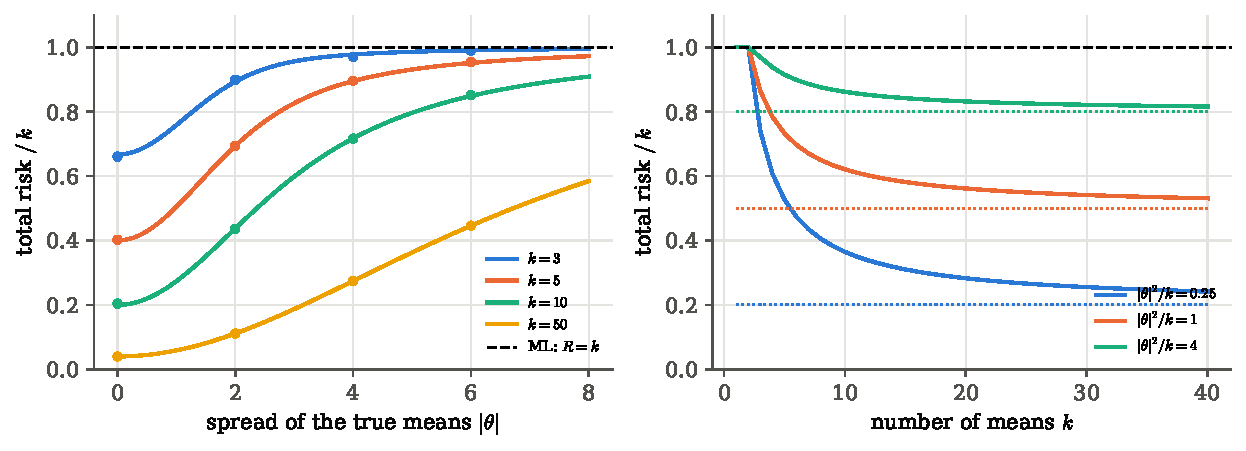
\includegraphics[width=\linewidth]{figures/chT5/james_stein.pdf}
\caption{Total risk of the James--Stein estimator divided by $k$ (the plain
readings give one, dashed). Left: against the length $|\params|$ of the
vector of true means, for $k=3,5,10,50$; curves are exact, dots are Monte
Carlo. Every curve starts at $2/k$ and rises towards one as the means spread
out. Right: against $k$, with the means spread so that $|\params|^2/k$ is
fixed; dotted lines are the empirical-Bayes limit $1-B=\tau^2/(1+\tau^2)$
with $\tau^2=|\params|^2/k$, reached for many means.}
\label{T5a:fig:james-stein}
\end{figure}

\Cref{T5a:fig:james-stein} shows the whole picture. The gain is largest when
the means are close together compared with the noise and when there are
many of them; it never turns into a loss. For a fixed spread per component,
the risk per component falls quickly with $k$ to the empirical-Bayes limit
$\tau^2/(1+\tau^2)$, the value an analyst who knew $\tau$ would get.

\subsection{When shrinkage is dangerous}
\label{T5a:sec:stein-danger}

\emph{The guarantee is for the total, not for each mean.} Take $k=\TFiveAOutK$
means, nine of them at zero and one, $\theta_1$, at a varying distance. The
nine are well described by ``all close together''; the tenth is not, but the
shrinkage factor is computed from all ten and pulls it in too.
\Cref{T5a:fig:js-outlier} shows the error of each. The nine benefit throughout.
The tenth is estimated \emph{worse} than by its own reading once $\theta_1$ is
more than about one unit away, with a mean squared error that peaks at
$\TFiveAOutMax$, nearly three times the error of its own reading, at
$\theta_1\approx\TFiveAOutAt$. The total, $\TFiveAOutTotal$ there, is still
below $10$, exactly as promised. If the tenth number is the one we care about,
say an anomalous detector or the one band power where new physics might show
up, we must not shrink it with the others.

\begin{figure}[htbp]
\centering
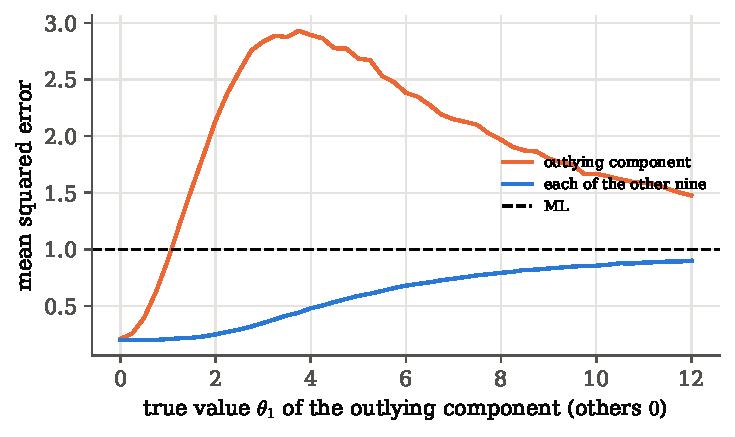
\includegraphics[width=0.65\linewidth]{figures/chT5/js_outlier.pdf}
\caption{James--Stein with $k=\TFiveAOutK$ means, nine at zero and one at
$\theta_1$. The nine (blue, each) always gain. The outlying one (orange)
loses once it is more than about one unit from the others, by up to a factor
of three, and recovers slowly as it moves so far away that the shrinkage
factor approaches one.}
\label{T5a:fig:js-outlier}
\end{figure}

\emph{The numbers must be exchangeable.} The empirical-Bayes reading assumed
that all $\theta_i$ come from one population. Shrinking a detector gain, a
galaxy luminosity and a band power towards a common value is legal
mathematics (the risk theorem holds for any $\params$) but useless: the
gain is large only when the true values really are close together, on the
same scale and with comparable noise. In practice one standardises each
reading by its noise and shrinks only quantities of the same kind.

\emph{Shrink towards a sensible point.} The origin in
\eqref{T5a:eq:james-stein} is arbitrary; any fixed point $\bm\mu_0$ works
with $\bm X$ replaced by $\bm X-\bm\mu_0$. Better still is the average of the
readings themselves: shrinking towards $\bar X$ uses one degree of freedom to
estimate the centre, and the factor becomes $(k-3)/\sum_i(X_i-\bar X)^2$,
which needs $k\ge4$ \cite{EfronMorris1975}.

\emph{Never shrink past the target.} When $|\bm X|^2<k-2$ the factor
$1-(k-2)/|\bm X|^2$ is negative and \eqref{T5a:eq:james-stein} flips every
sign, which is absurd. The \newterm{positive-part} estimator replaces the
factor by $\max(0,1-(k-2)/|\bm X|^2)$ \mainref{(12.12), p.~204}; it has lower
risk than James--Stein for every $\params$, and in the twenty-detector example
it gained a little, $\TFiveAEbRiskJSP$ against $\TFiveAEbRiskJS$.

\begin{pitfall}[Shrinkage changes the error bars too]
A shrunk estimate is biased, by $-B\,\theta_i$ on average for component $i$,
and its error bar is not $1$. Quoting $\hat\theta_i\pm1$ after shrinking
overstates the precision for the outliers and understates the gain for the
rest. The empirical-Bayes posterior gives a consistent error bar,
$\sqrt{1-B}$ plus a correction for the uncertainty in $B$ itself
\cite{EfronMorris1975}; a hierarchical model sampled with MCMC
(\cref{ch:09}) gives it automatically.
\end{pitfall}

\paragraph{When to use shrinkage.}
Use it when many quantities of the same kind are estimated with comparable
noise, when the total or typical error is what matters (a map of
calibrations, a catalogue of luminosities, the many entries of a
covariance matrix estimated from simulations), and when no single quantity
is singled out for discovery. Do not use it for the one number an
experiment exists to measure.
\section{Wild readings: robust estimators}
\label{T5a:sec:robust}

\paragraph{What we already have.}
The three laboratories of \cref{T5a:sec:questions} showed that a few wild
readings can make the sample mean five times worse than it needs to be, and
that the median resists them (\cref{3b:sec:efficiency}). We also saw the
best possible answer: maximum likelihood with the exact law of the noise,
which came within a few per cent of the Cram\'er--Rao bound in laboratory C.
And we met the picture that organises everything here: each estimator is a
balance of \emph{pulls} $\psi$, one per reading (\cref{T5a:fig:pull}).

\paragraph{When that is not enough.}
Maximum likelihood in laboratory C needed to know that $5\%$ of the readings
come from a Gaussian exactly ten times wider. In real data we never know
that. We know only that the instrument is mostly well behaved and that
something occasionally goes wrong: a cosmic ray, a glitch in a gravitational-wave
strain channel, a mistyped entry, a satellite crossing the field of view.
We want a recipe that is almost as good as the mean when nothing goes
wrong, and never catastrophic when something does.

\paragraph{A story with the whole trick in it.}
In a diving competition, seven judges each give a score, and the result is
the average of the five middle scores: the highest and the lowest are
dropped. One judge who favours a diver from their own country, or who
presses the wrong key, cannot move the result much, because an extreme
score is simply not counted. When all judges are honest, dropping two of
seven costs a little precision. When one is not, it saves the competition.
That is the whole idea of robustness: give up a little efficiency in the
ideal case to limit how much any single reading can do.

In physics the dishonest judges are outliers. A CCD exposure collects a
cosmic-ray hit in a few per cent of its pixels, always adding charge, never
removing it. A gravitational-wave detector has short loud glitches of
instrumental origin. An astronomer averaging repeated photometry ``clips''
readings more than three standard deviations from the median, and the
Bayesian answer to the same problem is a likelihood with heavier tails than
a Gaussian \srcref{HobsonBMC}{\S2.4, pp.~52--53}, \srcref{Sivia}{(3.72),
p.~67}. The idea of the section is to make ``limit the influence of any
single reading'' precise, measure it, and build estimators around it.

\paragraph{The story in symbols.}
Add one extra reading, of value $x$, to $n$ readings with mean $\bar x$. The
new mean is $(n\bar x+x)/(n+1)$, so it moves by
\begin{equation}
  \frac{n\bar x+x}{n+1}-\bar x=\frac{x-\bar x}{n+1} ,
  \label{T5a:eq:mean-shift}
\end{equation}
which grows without limit as $x$ does: one reading at a million moves the
mean by a million over $n+1$. The median moves by at most half the gap
between the two middle readings, whatever $x$ is. Between the two lies a
dial: Huber's estimator lets a reading pull like the mean while it is within
$k$ standard deviations of the centre, and with a constant pull beyond. With
$k=\TFiveARobK$ it is $\TFiveARobEff$ times as efficient as the mean for
Gaussian noise, a price of five per cent. In return, when $10\%$ of the
readings are wild (symmetric, ten times wider), its mean squared error is
$\TFiveARobSymTenHub/n$ against the mean's $\TFiveARobSymTenMean/n$, seven
times smaller. Lesson: bounding the pull of each reading costs little when
the data are clean and saves a great deal when they are not.

\paragraph{A picture: three ways to pull.}
\Cref{T5a:fig:rho-psi} draws, for three estimators, the penalty $\rho(e)$
that each reading pays for lying a distance $e$ from the estimate, and its
slope, the pull $\psi(e)=\rho'(e)$. The mean minimises $\sum_i\rho(x_i-\mu)$
with $\rho=\frac12e^2$, a parabola, so far readings pay enormously and pull
hard. The median minimises $\sum_i|x_i-\mu|$, a V, so every reading pulls
with the same strength. Huber's penalty is the parabola in the middle and
the V outside: it behaves like the mean for the bulk of the data and like
the median for the few readings far out.

\begin{figure}[htbp]
\centering
\begin{tikzpicture}
\begin{axis}[name=rho,width=6.4cm,height=4.8cm,xmin=-3.5,xmax=3.5,axis lines=middle,
  tick label style={font=\scriptsize},samples=141,domain=-3.5:3.5,
  ymin=0,ymax=4,xlabel={$e$},ylabel={penalty $\rho(e)$},
  xlabel style={anchor=north west},ylabel style={anchor=south},
  legend style={font=\scriptsize,draw=none,fill=white,at={(0.5,-0.22)},anchor=north},legend columns=3]
  \addplot[thick,formblue] {0.5*x^2}; \addlegendentry{mean: $\frac12e^2$}
  \addplot[thick,fibreorange] {abs(x)}; \addlegendentry{median: $|e|$}
  \addplot[thick,tangentgreen,dashed] {(abs(x)<=1.345)*0.5*x^2+(abs(x)>1.345)*(1.345*abs(x)-0.5*1.345^2)};
  \addlegendentry{Huber, $k=1.345$}
\end{axis}
\begin{axis}[at={($(rho.east)+(1.4cm,0)$)},anchor=west,width=6.4cm,height=4.8cm,
  xmin=-3.5,xmax=3.5,axis lines=middle,tick label style={font=\scriptsize},
  samples=141,domain=-3.5:3.5,ymin=-3,ymax=3,xlabel={$e$},ylabel={pull $\psi(e)=\rho'(e)$},
  xlabel style={anchor=north west},ylabel style={anchor=south}]
  \addplot[thick,formblue] {x};
  \addplot[thick,fibreorange,samples=281] {(x>0)-(x<0)};
  \addplot[thick,tangentgreen,dashed] {max(-1.345,min(1.345,x))};
  \draw[faint,dotted] (axis cs:1.345,-3) -- (axis cs:1.345,3);
  \draw[faint,dotted] (axis cs:-1.345,-3) -- (axis cs:-1.345,3);
\end{axis}
\end{tikzpicture}
\caption{Left: the penalty each reading pays for lying a distance $e$ (in
units of the noise width) from the estimate. Right: its slope, the pull the
reading exerts. The mean's pull grows without limit; the median's is the
same at every distance; Huber's grows like the mean's up to $|e|=k$ (dotted
lines) and is constant beyond.}
\label{T5a:fig:rho-psi}
\end{figure}

\paragraph{One idea, many names.}
Estimators defined by a penalty $\rho$, or by the balance of pulls
$\sum_i\psi(x_i-\mu)=0$, are \newterm{M-estimators}, ``maximum-likelihood
type'' because $\rho=-\ln f$ gives maximum likelihood
\srcref{CasellaBerger}{\S10.2.2, pp.~391--392}. The pull at distance $x$,
suitably normalised, is the \newterm{influence function} of Hampel
\cite{Hampel1974}. The fraction of wild readings an estimator can survive is
its \newterm{breakdown point}. Sigma clipping, trimmed means, Tukey's
biweight and the iteratively reweighted fits of the second half of the
chapter are all members of this family, and Huber's 1964 paper started it
\cite{Huber1964}.

We first measure the pull of one reading exactly, then use it to compute
the variance of any M-estimator, build Huber's estimator, measure how many
wild readings each estimator survives, and finally weigh the price against
the gain by simulation.

\subsection{The influence function}
\label{T5a:sec:influence}

\begin{workdef}[influence function]
Let $T(F)$ be what an estimator converges to when the readings follow the
distribution $F$ \unpack{for the mean, the population mean of $F$}. Mix in a
small fraction $\delta$ of readings that all sit at one value $x$,
$F_\delta=(1-\delta)F+\delta\,\Delta_x$, where $\Delta_x$ puts all its
probability at $x$. The \newterm{influence function}
is $\mathrm{IF}(x)=\lim_{\delta\to0}[T(F_\delta)-T(F)]/\delta$, the rate at
which the estimate moves per unit of contamination at $x$
\srcref{CasellaBerger}{Def.~10.6.1, p.~419}. Operationally: add one reading
at $x$ to a large sample of $n$ and multiply the change in the estimate by
$n+1$.
\end{workdef}

\emph{The mean.} The population mean of $F_\delta$ is $(1-\delta)\mu+\delta x$,
so $T(F_\delta)-T(F)=\delta(x-\mu)$ and $\mathrm{IF}(x)=x-\mu$: unbounded,
the finite-sample shift \eqref{T5a:eq:mean-shift} in the limit.

\emph{The median.} The median $m_\delta$ of $F_\delta$ is where its
cumulative distribution reaches one half. If $x$ lies above the median, the
added mass is not yet counted at $m_\delta$, so
\begin{align}
  (1-\delta)F(m_\delta)=\tfrac12
  &\eqby{1}\quad F(m_\delta)=\frac{1}{2(1-\delta)}=\tfrac12+\tfrac12\delta+O(\delta^2) \notag\\
  &\eqby{2}\quad m_\delta-m=\frac{\delta}{2f(m)}+O(\delta^2),
  \label{T5a:eq:if-median}
\end{align}
\begin{explain}
  \item Divide by $1-\delta$ and expand $1/(1-\delta)=1+\delta+O(\delta^2)$.
  \item Expand $F$ around the median $m$, where $F(m)=\frac12$: $F(m_\delta)=\frac12+f(m)(m_\delta-m)+\dots$, and solve.
\end{explain}
If $x$ lies below the median, the added mass is counted:
$(1-\delta)F(m_\delta)+\delta=\frac12$, and the same steps give
$m_\delta-m=-\delta/(2f(m))$. So
$\mathrm{IF}(x)=\sgn(x-m)/(2f(m))$ \srcref{CasellaBerger}{Ex.~10.6.2,
p.~419}: bounded, and the same for a reading just above the median as for
one at infinity.

\emph{Variances from influence.} An estimator is, for large $n$, its
limit plus the average of the influences of the individual readings,
$T\approx T(F)+\frac1n\sum_i\mathrm{IF}(x_i)$, so its variance is
$\E[\mathrm{IF}(X)^2]/n$. For the mean this is $\sigma^2/n$. For the median
it is $\E[1/(4f(m)^2)]/n=1/(4nf(m)^2)$, the formula used throughout
\cref{T5a:sec:questions}. The influence function therefore measures two
things at once: how much one bad reading can do (its largest value), and
how precise the estimator is on good data (its mean square).

\subsection{M-estimators: one pull, one variance}
\label{T5a:sec:m-estimators}

An M-estimator solves $\sum_i\psi(x_i-\hat\mu)=0$
\srcref{CasellaBerger}{(10.2.3), p.~392}. Take $\psi$ odd and $F$ symmetric
about $\mu$, so that $\E_F\psi(X-\mu)=0$ and the population version of the
equation is solved by the true centre. Under $F_\delta$ the solution
$\mu_\delta$ satisfies
\begin{align}
  0&\eqby{1}(1-\delta)\,\E_F\psi(X-\mu_\delta)+\delta\,\psi(x-\mu_\delta) \notag\\
  &\eqby{2}(1-\delta)\bigl[\E_F\psi(X-\mu)-(\mu_\delta-\mu)\,\E_F\psi'(X-\mu)\bigr]+\delta\,\psi(x-\mu)+O(\delta^2) \notag\\
  &\eqby{3}-(\mu_\delta-\mu)\,\E_F\psi'(X-\mu)+\delta\,\psi(x-\mu)+O(\delta^2),
  \label{T5a:eq:m-if-derivation}
\end{align}
\begin{explain}
  \item The estimating equation, averaged over the mixture $F_\delta$.
  \item Expand $\psi(X-\mu_\delta)$ to first order in the small shift $\mu_\delta-\mu$; in the last term the shift only adds $O(\delta^2)$.
  \item $\E_F\psi(X-\mu)=0$, and $\mu_\delta-\mu$ is itself of order $\delta$, so $\delta(\mu_\delta-\mu)$ is $O(\delta^2)$.
\end{explain}
Dividing by $\delta$ and letting $\delta\to0$ gives
$\mathrm{IF}(x)=\psi(x-\mu)/\E\psi'(X-\mu)$, and the variance rule of
\cref{T5a:sec:influence}, $\E[\mathrm{IF}^2]/n$, then gives
$n\Var\hat\mu=\E\psi^2/(\E\psi')^2$.
\begin{keyidea}[Influence and variance of an M-estimator]
The M-estimator with pull $\psi$ has
$\mathrm{IF}(x)=\psi(x-\mu)/\E\psi'(X-\mu)$ and, for large $n$,
$n\Var\hat\mu=\E\psi^2/(\E\psi')^2$. Its influence is the pull itself,
rescaled; a bounded pull means a bounded influence.
\end{keyidea}
\noindent This variance is the formula of \srcref{CasellaBerger}{(10.2.6),
p.~393}, which they derive instead by a Taylor expansion of the estimating
equation. Two checks: $\psi(e)=e$ gives $\E\psi'=1$ and $n\Var=\sigma^2$, the
mean. $\psi=\sgn$ gives $\psi'=2\,\delta_{\mathrm D}(e)$ (the jump of height
two at zero, $\delta_{\mathrm D}$ the Dirac delta), so $\E\psi'=2f(\mu)$ and
$n\Var=1/(4f(\mu)^2)$, the median.

\paragraph{Example: no M-estimator beats maximum likelihood.}
Integrating by parts, with $f$ the noise density and
$s(e)=-f'(e)/f(e)$ the maximum-likelihood pull,
\begin{equation}
  \E\psi'
  \eqby{1}\int\psi'(e)f(e)\,\dd e
  \eqby{2}-\int\psi(e)f'(e)\,\dd e
  \eqby{3}\E[\psi\,s]
  \relby{4}{\le}\sqrt{\E\psi^2}\sqrt{\E s^2}=\sqrt{\E\psi^2\,I},
  \label{T5a:eq:m-cs}
\end{equation}
\begin{explain}
  \item Definition of the expectation.
  \item Integration by parts; $\psi f$ vanishes at $\pm\infty$.
  \item $-f'=s\,f$.
  \item Cauchy--Schwarz, and $\E s^2=I$ is the Fisher information of one reading.
\end{explain}
so $n\Var\hat\mu=\E\psi^2/(\E\psi')^2\ge1/I$, with equality only when
$\psi\propto s$: an M-estimator reaches the Cram\'er--Rao bound only if its
pull is the maximum-likelihood pull of the true noise law
\srcref{CasellaBerger}{(10.2.9), p.~394}. Robustness is bought with
efficiency, never the other way round.

\subsection{Huber's estimator}
\label{T5a:sec:huber}

Huber's penalty is \srcref{CasellaBerger}{(10.2.2), p.~391}
\begin{equation}
  \rho_k(e)=\begin{cases}\frac12e^2,&|e|\le k,\\[2pt] k|e|-\frac12k^2,&|e|>k,\end{cases}
  \qquad
  \psi_k(e)=\rho_k'(e)=\begin{cases}-k,&e<-k,\\ e,&|e|\le k,\\ k,&e>k,\end{cases}
  \label{T5a:eq:huber-psi}
\end{equation}
with the constant $-\frac12k^2$ chosen so that the two pieces of $\rho_k$
meet at $|e|=k$ with the same value and the same slope. The readings are
measured in units of the noise width, $e=(x_i-\mu)/\hat\sigma$, where
$\hat\sigma$ must itself be robust; the usual choice is the median absolute
deviation from the median, divided by $0.6745$ so that it estimates $\sigma$
for Gaussian data. The estimate $\hat\mu$ minimises $\sum_i\rho_k(e_i)$.

\emph{Where does this shape come from?} It is maximum likelihood for a
particular noise law: $\psi_k=-(\ln f_0)'$ for
$f_0(e)\propto e^{-\rho_k(e)}$, a density that is Gaussian in the centre and
exponential (Laplace-like) in the tails. Huber showed that among all
contaminated Gaussians $(1-\epsilon)\Normal(0,1)+\epsilon H$, with $H$
anything at all, this $f_0$ is the hardest one to estimate a centre from,
and that its maximum-likelihood estimator has the smallest worst-case
variance over the whole family \cite{Huber1964}. The tuning constant and the
contamination are linked by $2\varphi(k)/k-2[1-\Phi(k)]=\epsilon/(1-\epsilon)$,
with $\varphi,\Phi$ the standard Gaussian density and distribution
function; $k=\TFiveARobK$ corresponds to $\epsilon=\TFiveARobEpsLF$.

\paragraph{Example: the price at Gaussian noise.}
For $\Normal(0,1)$ noise and the variance formula of the key idea above,
$\E\psi_k'=\Prob(|Z|\le k)=2\Phi(k)-1$, and
\begin{align}
  \E\psi_k^2
  &\eqby{1}\int_{-k}^{k}z^2\varphi(z)\,\dd z+2k^2\bigl[1-\Phi(k)\bigr]
   \eqby{2}\bigl[2\Phi(k)-1\bigr]-2k\varphi(k)+2k^2\bigl[1-\Phi(k)\bigr],
  \label{T5a:eq:huber-epsi2}
\end{align}
\begin{explain}
  \item Inside $|z|\le k$ the pull is $z$; outside it is $\pm k$, on two tails of probability $1-\Phi(k)$ each.
  \item Integrate by parts with $z\varphi(z)=-\varphi'(z)$: $\int_{-k}^kz\cdot z\varphi\,\dd z=[-z\varphi]_{-k}^k+\int_{-k}^k\varphi\,\dd z=-2k\varphi(k)+2\Phi(k)-1$.
\end{explain}
For $k=\TFiveARobK$: $\E\psi_k'=\TFiveARobPpsi$ and
$\E\psi_k^2=\TFiveARobEpsiTwo$, so $n\Var\hat\mu=\TFiveARobEpsiTwo/\TFiveARobPpsi^2$
and the efficiency relative to the mean is
$(\E\psi_k')^2/\E\psi_k^2=\TFiveARobEff$. This is why $1.345$ is the
standard choice: exactly a $5\%$ loss at the Gaussian.

\emph{Computing it.} $\sum_i\rho_k(e_i)$ is a convex function of $\mu$ (each
term is), so it has one minimum, where its slope $-\frac{1}{\hat\sigma}\sum_i\psi_k(e_i)$
crosses zero. The sum $\sum_i\psi_k((x_i-\mu)/\hat\sigma)$ never increases as
$\mu$ increases, is positive below the smallest reading and negative above
the largest, so the root can be found by bisection:

\pyfile[firstline=39,lastline=51,firstnumber=39]{code/chT5/lib_t5a.py}{Huber's estimate by bisection on the balance of pulls}

Line 44 takes the scale from the median absolute deviation (or a known
scale, if given). Line 45 brackets the root between the smallest and largest
reading. Each pass of the loop (lines 46--50) evaluates the total pull at the
midpoint and keeps the half of the bracket where the pull changes sign;
sixty halvings make the bracket negligibly small. The second half of the
chapter computes the same estimate a different way, as a weighted mean whose
weights are recomputed until they stop changing.

\paragraph{Example: eight good readings and three outliers.}
\srcref{CasellaBerger}{Ex.~10.2.5, p.~391} uses eight standard Gaussian
readings plus three outliers, $3$, $6$ and $9$, with mean $\TFiveARobCBMean$
and median $\TFiveARobCBMed$. Minimising their criterion with the scale fixed
at one gives, for $k=1,2,3,4,5,6$, the estimates $\TFiveARobCBkOne$,
$\TFiveARobCBkTwo$, $\TFiveARobCBkThree$, $\TFiveARobCBkFour$,
$\TFiveARobCBkFive$ and $\TFiveARobCBkSix$, moving steadily from the median
towards the mean as $k$ grows; from $k=8$ on, every residual is below $k$ and
the estimate is the mean.\footnote{The table printed with this example in
\srcref{CasellaBerger}{Table~10.2.3} gives different intermediate values
(e.g.\ $-0.04$ at $k=2$ and $0.97$ at $k=8$). Its values cannot be minima of
the stated criterion: at $k=2$ the eight good readings minus $0.34$ have
pulls summing to $-6.00$ and the three outliers each pull $+2$, so $0.34$
balances; and at $k=8$ the largest residual from the mean, $9-1.34$, is below
$8$, so the minimum is the mean itself.} The point of the example survives:
$k$ is a dial between the median ($k\to0$) and the mean ($k\to\infty$).

\subsection{Breakdown: how many wild readings an estimator survives}
\label{T5a:sec:breakdown}

The influence function describes one reading at a time. The opposite
extreme asks how many readings can go bad together. The
\newterm{breakdown point} of an estimator is the largest fraction of the
readings that can be moved to arbitrary values (to infinity) while the
estimate stays bounded \srcref{CasellaBerger}{Def.~10.2.2, p.~389}. The mean breaks with one reading, by \eqref{T5a:eq:mean-shift}: its
breakdown point is $0$. The median survives as long as fewer than half the
readings are moved, because the middle reading is then still one of the
original ones, trapped between the smallest and largest of them: breakdown
point $\frac12$, the best possible (beyond half, nobody can say which
readings are the good ones). A trimmed mean that drops the $\alpha$ fraction
at each end survives until more than that fraction is moved: breakdown point
$\alpha$. Huber's estimator with a fixed scale has a bounded pull, but the
scale must also survive; with the median absolute deviation, which itself
breaks only at one half, the breakdown point is $\frac12$.

The right panel of \cref{T5a:fig:influence} shows this on a sample of
$\TFiveARobNzero$ readings, replacing $m$ of them by $1000$. The mean breaks at
$m=\TFiveARobBreakMean$, the $10\%$ trimmed mean at $m=\TFiveARobBreakTrim$
(it drops two from each end), and the median and Huber's estimator only at
$m=\TFiveARobBreakMed$, half the sample. The left panel shows the influence
functions as finite-sample sensitivity curves: one reading added at $x$ to a
typical sample (the $\TFiveARobNzero$ quantiles of a Gaussian). The mean's
curve is a straight line; the others level off, Huber's at
$\pm k/\E\psi_k'=\pm\TFiveARobK/\TFiveARobPpsi$, as the key idea predicts.

\begin{figure}[htbp]
\centering
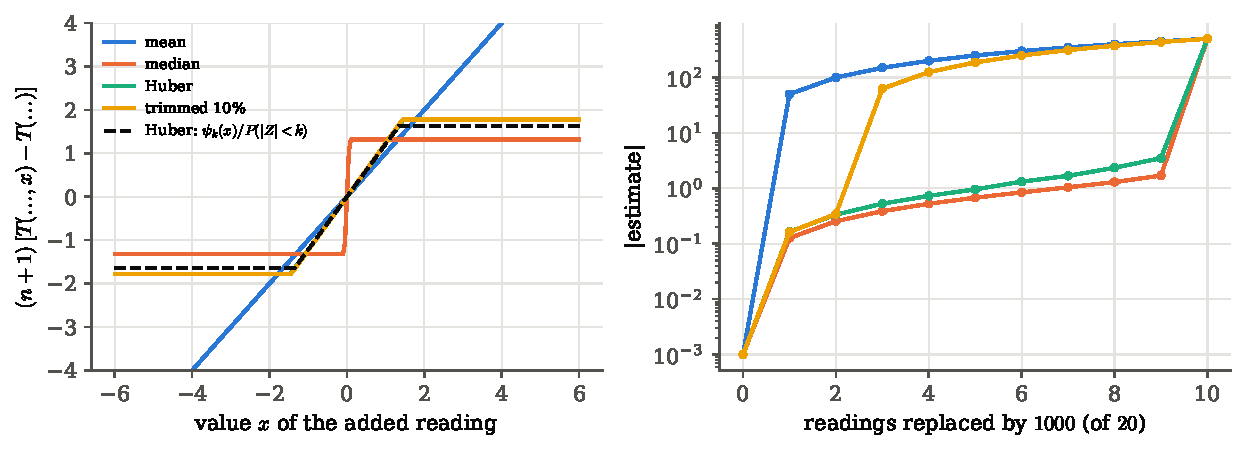
\includegraphics[width=\linewidth]{figures/chT5/influence.pdf}
\caption{Left: how far one extra reading at $x$ moves four estimators of the
centre of $\TFiveARobNzero$ Gaussian readings, times $n+1$ (the finite-sample
influence function). Only the mean follows the reading out without limit;
the dashed line is Huber's influence function $\psi_k(x)/\E\psi_k'$. Right:
breakdown. The estimate as $m$ of the $\TFiveARobNzero$ readings are replaced
by $1000$, on a logarithmic scale. The mean jumps at once, the trimmed mean
after three, the median and Huber's estimator only at ten.}
\label{T5a:fig:influence}
\end{figure}

\subsection{The price and the gain, side by side}
\label{T5a:sec:robust-sim}

The script \pyname{code/chT5/05_robust.py} draws $\TFiveARobM$ samples of
$n=\TFiveARobN$ readings from a unit Gaussian, replaces a fraction $\epsilon$
of them by wild readings, and compares four estimators of the centre (true
value zero). The wild readings are either symmetric, $\Normal(0,10^2)$, or
one-sided like cosmic rays, $|\Normal(0,10^2)|$, which only ever add.
\Cref{T5a:fig:robust-mse} shows $n$ times the mean squared error.

\begin{figure}[htbp]
\centering
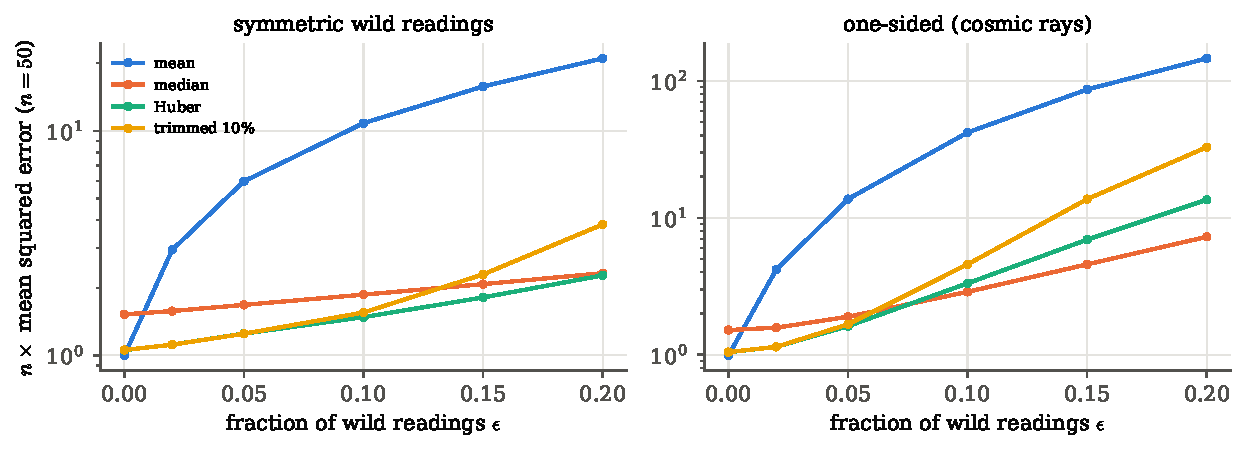
\includegraphics[width=\linewidth]{figures/chT5/robust_mse.pdf}
\caption{$n$ times the mean squared error of four estimators of a centre
($n=\TFiveARobN$), against the fraction $\epsilon$ of wild readings.
Left: wild readings symmetric about the centre. Right: wild readings that
only add, like cosmic rays. At $\epsilon=0$ the mean is best, Huber's
estimator and the trimmed mean lose $5\%$, the median $50\%$. With
contamination the mean is soon the worst by an order of magnitude.}
\label{T5a:fig:robust-mse}
\end{figure}

\emph{No contamination.} The mean gives $\TFiveARobGMean$, Huber's estimator
$\TFiveARobGHub$ and the trimmed mean $\TFiveARobGTrim$ (both five per cent
worse, as computed above for Huber), the median $\TFiveARobGMed$, close to
$\pi/2$. This is the price of protection.

\emph{Symmetric contamination.} With $10\%$ wild readings the mean reaches
$\TFiveARobSymTenMean$, while Huber's estimator gives $\TFiveARobSymTenHub$,
the trimmed mean $\TFiveARobSymTenTrim$ and the median $\TFiveARobSymTenMed$.
Symmetric outliers do not bias any of the four; they only inflate the
variance, and the bounded pulls stop them from doing so.

\emph{One-sided contamination.} Now every estimator is biased, because the
contaminated distribution itself has moved: there is no longer a unique
``centre'' for an estimator to find, and each estimator settles somewhere
between the core and the outliers. With $5\%$ cosmic rays the mean's error,
$\TFiveARobOneFiveMean$, is dominated by its bias; Huber's estimator
($\TFiveARobOneFiveHub$), the trimmed mean ($\TFiveARobOneFiveTrim$) and the
median ($\TFiveARobOneFiveMed$) are hardly hurt. At $20\%$ the ordering
changes: the median, $\TFiveARobOneTwentyMed$, beats Huber's estimator,
$\TFiveARobOneTwentyHub$, because the bias of an estimator under a small
contamination is roughly $\epsilon$ times the largest value of its
influence function, and the median's largest influence,
$\sqrt{2\pi}/2\approx1.25$, is smaller than Huber's,
$\TFiveARobK/\TFiveARobPpsi\approx1.64$. (The mean, at
$\TFiveARobOneTwentyMean$, is off the scale of usefulness.)

\begin{pitfall}[Robust is not the same as right]
A robust estimator limits the damage of readings that do not fit the model;
it does not explain them. With one-sided contamination it is still biased,
only less so. If the outliers have a physical cause (cosmic rays, a glitch
population), the best answer models that cause, either by flagging the
readings with independent information (a cosmic-ray detection algorithm, a
glitch veto) or by a likelihood that contains the contaminating population,
as maximum likelihood did in laboratory C. And never simply delete readings
because they disagree with the answer one expected: that is a selection
effect, and it makes error bars too small.
\end{pitfall}

\paragraph{When to use a robust estimator.}
Use it when the bulk of the noise is understood but rare failures are not:
as a default for repeated readings of one quantity, for a first fit that
identifies outliers before a careful analysis, and whenever an analysis must
run unsupervised on data no one will inspect reading by reading. Choose the
median when as many as a third of the readings may be bad, Huber's estimator
(or a trimmed mean) when a few per cent may be, and maximum likelihood with
an explicit contamination model when the failures are understood well
enough to describe.
\section{When the parameter lives in the covariance: quadratic estimators}
\label{T5a:sec:quadratic}

\paragraph{What we already have.}
Every estimator so far found a parameter that \emph{shifts} the data: a
level $\mu$, a pair of masses, the coefficients of a fit. Those live in the
mean of the data, $\E\data=\mathbf A\params$, and a weighted sum of the
readings can pick them out. We have also met, case by case, parameters of a
different kind. The angular power spectrum $C_\ell$ was estimated by
averaging the squares of the harmonic coefficients, with the noise power
subtracted (\cref{7b:eq:chat,7b:eq:noise-bias}). Masked skies needed the
pseudo-$C_\ell$ machinery of \cref{8b:sec:master}, and \cref{8a:eq:qml}
quoted a ``quadratic maximum-likelihood'' formula as one Newton step of the
likelihood.

\paragraph{When that is not enough.}
A parameter that sets how much the data \emph{scatter} has no effect on
their mean: the sky fluctuations average to zero whatever their amplitude.
So no linear combination of the readings carries information about it on
average, and the estimator must be at least quadratic. What is the best
quadratic combination, when the sky is masked and the noise differs from
pixel to pixel? And something new happens to the noise, which the next story
makes plain.

\paragraph{A story with the whole trick in it.}
A camera on a wooden pier films a moored boat. Suppose we want the boat's
average height above the water. Each frame is off a little because the pier
shakes, sometimes up and sometimes down, and a long film averages the
shaking away. Now suppose instead we want to know \emph{how much the boat
rocks}. Every frame shows the boat's motion and the pier's motion added
together, and their spreads add too. However long we film, the pier's wobble
never cancels: it adds the same amount of apparent rocking in every frame,
and a longer film only measures the total, boat plus pier, more precisely. To
learn how much the boat rocks we must know how much the pier shakes, and
\emph{subtract} it.

That is the difference between estimating a fixed number and estimating a
variance. When the target is a fixed number, noise moves each reading in
either direction and its effect averages out; it widens the error bar and
nothing more. When the target is a variance or a power spectrum, the
noise's own variance lands on top of the signal's in every reading, so
the same noise now pushes every estimate the same way: it has become a
\emph{bias}, and it must be computed and subtracted. A CMB experiment
subtracts the detector noise power from the measured spectrum
(\cref{7b:eq:noise-bias}); a lensing reconstruction subtracts the
reconstruction noise $N_0$ from the spectrum of the lensing map
(\cref{T1b:sec:recon}). The idea of the section is that both are the
constant term of one general recipe, a quadratic form of the data minus a
noise bias, and that the recipe has a best version whose error is set by
the Fisher matrix.

\paragraph{The story in symbols: one pixel.}
A single pixel holds a signal $s$ of variance $p$, the parameter, plus
independent noise of known variance $\sigma^2$. Its reading
$x=s+n$ has mean zero and variance $p+\sigma^2$. The natural estimate of $p$
is the square of the reading, minus a constant $b$:
\begin{align}
  \E(x^2-b)&\eqby{1}p+\sigma^2-b,\notag\\
  \Var(x^2-b)&\eqby{2}\E x^4-(\E x^2)^2\eqby{3}3(p+\sigma^2)^2-(p+\sigma^2)^2=2(p+\sigma^2)^2 .
  \label{T5a:eq:one-pixel}
\end{align}
\begin{explain}
  \item $\E x^2=\Var x$ because $\E x=0$; signal and noise variances add for independent pieces.
  \item A constant does not change a variance.
  \item For a Gaussian of variance $v$, $\E x^4=3v^2$ (the case of \cref{7a:eq:wick} with all four indices equal).
\end{explain}
The dial is $b$. The naive choice $b=0$ is biased by exactly $\sigma^2$, the
noise variance, however many pixels we average. The choice $b=\sigma^2$
removes the bias. The price that cannot be removed is in the variance:
$2(p+\sigma^2)^2$ contains the noise too, so a noisy pixel gives a poor
estimate of $p$ even after debiasing. With $p=1$ and $\sigma^2=0.5$ the
script \pyname{code/chT5/06_quadratic.py} finds, over $\TFiveAQM$ draws, a
mean of $\TFiveAQaNaive$ for $x^2$ and $\TFiveAQaMean$ for $x^2-\sigma^2$, and
a variance of $\TFiveAQaVar$ (prediction $\TFiveAQaVarTh$); the left panel of
\cref{T5a:fig:quadratic} shows the two distributions. Lesson: for a variance
parameter the noise appears twice, once as a bias we can subtract and once
as extra scatter we cannot.

\paragraph{A picture: the cloud of readings.}
With two pixels, plot each pair of readings $(x_1,x_2)$ as a point. With no
noise and independent signal of variance $p$ in each, the points form a round
cloud of radius about $\sqrt p$; the parameter is the \emph{size} of the
cloud, and its centre is always the origin, so the average position of the
points says nothing about $p$. Noise stretches the cloud, more along the
noisier pixel's axis (\cref{T5a:fig:cloud}). An estimate of the size must
use squared distances, and it should trust the direction in which the
stretching by noise is small. That is the whole design problem for
quadratic estimators: which squared combinations to use, with what weights,
and what to subtract.

\begin{figure}[htbp]
\centering
\begin{tikzpicture}[scale=0.85]
  \draw[faint,->] (-3.4,0) -- (3.6,0) node[right,black] {$x_1$};
  \draw[faint,->] (0,-3.0) -- (0,3.2) node[above,black] {$x_2$};
  \draw[formblue,thick] (0,0) circle (1);
  \draw[fibreorange,thick,dashed] (0,0) ellipse (1 and 2);
  \node[lbl,formblue,anchor=west] at (1.05,-0.5) {signal only: radius $\sqrt p=1$};
  \node[lbl,fibreorange,anchor=west] at (0.85,1.75) {with noise: semi-axes $1$ and $2$};
  \node[lbl,align=right,anchor=north east] at (-1.25,-1.9) {pixel 1 noiseless,\\ pixel 2 noise variance $3$};
\end{tikzpicture}
\caption{Two pixels whose signals are independent with variance $p=1$. The
signal alone fills a round cloud of radius one (blue, one standard
deviation). Noise of variance $3$ in the second pixel stretches the cloud to
a standard deviation of $2$ along $x_2$ (orange, dashed). Both clouds are
centred at the origin, so only the squared readings carry information about
$p$, and the squared reading of the noisy pixel carries much less of it.}
\label{T5a:fig:cloud}
\end{figure}

\paragraph{One idea, many names.}
A quadratic form of the data minus a constant is the general shape of every
variance or spectrum estimator: the sample variance of \cref{3a:eq:s2}, the
full-sky $\Chat$, the band powers of a galaxy survey, the pseudo-$C_\ell$ of
a masked map, the cross-spectrum of two detectors, and the lensing
reconstruction, which is quadratic in the CMB temperature
\cite{HuOkamoto2002}. Its best version is the \newterm{quadratic
maximum-likelihood} (QML) estimator \cite{Tegmark1997QML}, whose weights are
built from the inverse covariance and whose normalisation is the Fisher
matrix. The constant subtracted goes by many names, noise bias,
$N_\ell$, $N_0$, but it is always the same object: what the quadratic form
would give if the data contained noise alone.

We set up the general quadratic estimator, derive its mean (the
unbiasedness condition and the bias term) and its variance for Gaussian
data, find the weights that minimise the variance, and test them on the two
pixels, on the full sky and on a masked field with uneven noise.

\subsection{Quadratic estimators and their noise bias}
\label{T5a:sec:quad-mean}

Let the data $\data$ (pixels, Fourier modes, any list of $N$ numbers) have
mean zero and a covariance that is a sum of known templates, one per
parameter, plus noise:
\begin{equation}
  \Cov\data=\Cmat=\sum_ap_a\Cmat_a+\mathbf N .
  \label{T5a:eq:cov-model}
\end{equation}
For a power spectrum, $p_a$ is the band power in band $a$ and $\Cmat_a$ is
the covariance a unit band power would produce in the pixels: it encodes the
geometry, the mask and the beam. $\mathbf N$ is the noise covariance.

\begin{workdef}[quadratic estimator]
A \newterm{quadratic estimator} of $p_a$ is $\hat q_a=\data\T\mathbf E_a\data-b_a$,
with a symmetric $N\times N$ weight matrix $\mathbf E_a$ \unpack{which
products $d_id_j$ to add up, and with what weight} and a constant $b_a$, the
\newterm{noise bias}. For the one-pixel example, $\mathbf E=1$ and
$b=\sigma^2$.
\end{workdef}

\emph{Its mean.} For any data of mean zero, Gaussian or not,
\begin{equation}
  \E\,\data\T\mathbf E\data
  \eqby{1}\sum_{i,j}E_{ij}\,\E\,d_id_j
  \eqby{2}\sum_{i,j}E_{ij}C_{ji}
  \eqby{3}\tr(\mathbf E\Cmat),
  \label{T5a:eq:quad-mean}
\end{equation}
\begin{explain}
  \item Write the quadratic form as a double sum; expectation is linear.
  \item $\E d_id_j=C_{ij}=C_{ji}$ for mean-zero data.
  \item $\sum_jE_{ij}C_{ji}$ is the $(i,i)$ entry of $\mathbf E\Cmat$, and summing over $i$ gives the trace.
\end{explain}
so, with \eqref{T5a:eq:cov-model},
$\E\hat q_a=\sum_bp_b\tr(\mathbf E_a\Cmat_b)+\tr(\mathbf E_a\mathbf N)-b_a$.
The estimate is unbiased for $p_a$, whatever the true values of all the
parameters, exactly when
\begin{equation}
  \tr(\mathbf E_a\Cmat_b)=\delta_{ab}\quad\text{for every }b,
  \qquad b_a=\tr(\mathbf E_a\mathbf N) .
  \label{T5a:eq:trace-condition}
\end{equation}
The first condition makes the estimator respond to its own band with unit
weight and be blind to the others. The second is the noise bias: the value
the quadratic form takes, on average, when the data contain noise alone. It
does not shrink with more data; it is a fixed offset that must be known and
removed.

\subsection{The variance of a quadratic form of Gaussian data}
\label{T5a:sec:quad-var}

For Gaussian data the four-point average of the readings is the sum over
the three ways of pairing them (Isserlis' theorem, \cref{7a:eq:wick}),
$\E\,d_id_jd_kd_l=C_{ij}C_{kl}+C_{ik}C_{jl}+C_{il}C_{jk}$. Then, for two
symmetric weight matrices,
\begin{align}
  \E\bigl[(\data\T\mathbf E\data)(\data\T\mathbf E'\data)\bigr]
  &\eqby{1}\sum_{ijkl}E_{ij}E'_{kl}\bigl(C_{ij}C_{kl}+C_{ik}C_{jl}+C_{il}C_{jk}\bigr) \notag\\
  &\eqby{2}\tr(\mathbf E\Cmat)\tr(\mathbf E'\Cmat)+2\tr(\mathbf E\Cmat\mathbf E'\Cmat),
  \notag\\
  \Cov\bigl(\data\T\mathbf E\data,\data\T\mathbf E'\data\bigr)
  &\eqby{3}2\tr(\mathbf E\Cmat\mathbf E'\Cmat) .
  \label{T5a:eq:quad-var}
\end{align}
\begin{explain}
  \item Expand both quadratic forms and insert the three pairings.
  \item The first pairing gives $\sum_{ij}E_{ij}C_{ij}\sum_{kl}E'_{kl}C_{kl}$, a product of traces. The second gives $\sum E_{ij}C_{jl}E'_{lk}C_{ki}$ after using the symmetry $E'_{kl}=E'_{lk}$, which is $\tr(\mathbf E\Cmat\mathbf E'\Cmat)$; the third gives the same after using $C_{jk}=C_{kj}$.
  \item Subtract the product of the means \eqref{T5a:eq:quad-mean}. The constants $b_a$ do not change covariances.
\end{explain}
For one pixel, $\mathbf E=1$ and $\Cmat=p+\sigma^2$, this is
$2(p+\sigma^2)^2$, the result of \eqref{T5a:eq:one-pixel}. Note that the
\emph{total} covariance $\Cmat$, noise included, appears: the noise adds
scatter even after its bias is removed.

\subsection{The minimum-variance quadratic estimator}
\label{T5a:sec:qml}

\emph{One parameter first.} Among all symmetric $\mathbf E$ with
$\tr(\mathbf E\Cmat_a)=1$, which has the smallest variance
$2\tr(\mathbf E\Cmat\mathbf E\Cmat)$? Change $\mathbf E$ by a small symmetric
$\delta\mathbf E$. The variance changes by
$2\tr(\delta\mathbf E\,\Cmat\mathbf E\Cmat)+2\tr(\mathbf E\Cmat\,\delta\mathbf E\,\Cmat)
=4\tr(\delta\mathbf E\,\Cmat\mathbf E\Cmat)$ (the two terms are equal by the
cyclic property of the trace), and the constraint by
$\tr(\delta\mathbf E\,\Cmat_a)$. At the minimum, every change that keeps the
constraint must leave the variance unchanged, which with a Lagrange
multiplier $\lambda$ (as in \cref{3a:sec:blue}) means
$4\Cmat\mathbf E\Cmat=\lambda\Cmat_a$. Hence
\begin{equation}
  \mathbf E_a\eqby{1}\frac\lambda4\,\Cmat^{-1}\Cmat_a\Cmat^{-1}
  \eqby{2}\frac{\Cmat^{-1}\Cmat_a\Cmat^{-1}}{\tr(\Cmat^{-1}\Cmat_a\Cmat^{-1}\Cmat_a)},
  \qquad
  \Var\hat q_a\eqby{3}\frac{2}{\tr(\Cmat^{-1}\Cmat_a\Cmat^{-1}\Cmat_a)}=\frac{1}{F_{aa}},
  \label{T5a:eq:qml-one}
\end{equation}
\begin{explain}
  \item Multiply $4\Cmat\mathbf E\Cmat=\lambda\Cmat_a$ by $\Cmat^{-1}$ on both sides.
  \item Fix $\lambda$ by the constraint $\tr(\mathbf E_a\Cmat_a)=1$.
  \item Insert into $2\tr(\mathbf E\Cmat\mathbf E\Cmat)$: the factors $\Cmat\Cmat^{-1}$ cancel, leaving $2\tr(\Cmat^{-1}\Cmat_a\Cmat^{-1}\Cmat_a)$ over the square of the same trace.
\end{explain}
where $F_{ab}=\frac12\tr(\Cmat^{-1}\Cmat_a\Cmat^{-1}\Cmat_b)$ is the Fisher
matrix of Gaussian data whose covariance depends on the parameters
(\cref{10a:eq:gauss-fisher} with a mean that does not depend on them). So the
best quadratic estimator of one parameter, with the others known, reaches
the Cram\'er--Rao bound $1/F_{aa}$. The weights
$\Cmat^{-1}\Cmat_a\Cmat^{-1}$ read naturally: first whiten the data by
$\Cmat^{-1}$, which down-weights noisy and redundant pixels, then project
onto the pattern $\Cmat_a$ that the parameter produces.

\emph{All parameters together.} With several band powers unknown at once,
use the same building blocks for every band,
\begin{equation}
  \tilde q_a=\tfrac12\,\data\T\Cmat^{-1}\Cmat_a\Cmat^{-1}\data-\tfrac12\tr(\Cmat^{-1}\Cmat_a\Cmat^{-1}\mathbf N),
  \qquad
  \hat{\bm p}=\Fish^{-1}\tilde{\bm q} .
  \label{T5a:eq:qml}
\end{equation}
By \eqref{T5a:eq:quad-mean}, $\E\tilde q_a=\sum_bF_{ab}p_b$: each
$\tilde q_a$ responds to all the bands, mixed by the Fisher matrix, and
$\Fish^{-1}$ unmixes them, so $\E\hat{\bm p}=\bm p$. By
\eqref{T5a:eq:quad-var},
$\Cov(\tilde q_a,\tilde q_b)=2\cdot\frac14\tr(\Cmat^{-1}\Cmat_a\Cmat^{-1}\Cmat\,\Cmat^{-1}\Cmat_b\Cmat^{-1}\Cmat)=F_{ab}$,
so $\Cov\hat{\bm p}=\Fish^{-1}\Fish\Fish^{-1}=\Fish^{-1}$.
\begin{keyidea}[Quadratic maximum likelihood]
For Gaussian data with covariance $\sum_ap_a\Cmat_a+\mathbf N$, the estimator
\eqref{T5a:eq:qml} is unbiased and has covariance $\Fish^{-1}$, the
Cram\'er--Rao bound, when $\Cmat$ is evaluated at the true parameters. It is
the quadratic analogue of the Gauss--Markov estimator: whiten by
$\Cmat^{-1}$, project, subtract the noise bias, and unmix with the inverse
Fisher matrix.
\end{keyidea}

The weights need $\Cmat$, which contains the unknown $\bm p$. In practice one
evaluates $\Cmat$ at a fiducial guess. The estimate stays unbiased for any
guess, since \eqref{T5a:eq:quad-mean} holds with $\Fish$ computed from the
same guess, but it reaches $\Fish^{-1}$ only when the guess is right. This
is \cref{8a:eq:qml} read as one Newton step of the likelihood from the
fiducial spectrum, and \srcref{HobsonBMC}{\S10.2.3, p.~237} describes the same
Newton--Fisher iteration. Iterating it is the subject of the second half of
the chapter.

\paragraph{Example: two pixels, one of them noisy.}
Take the two pixels of \cref{T5a:fig:cloud}: independent signal of variance
$p=1$ in each, so $\Cmat_p=\Id$, and noise variances $0$ and $3$, so
$\Cmat=\diag(1,4)$. The plain average of the two debiased squares,
$\mathbf E=\diag(\frac12,\frac12)$ with $b=\frac32$, has, by
\eqref{T5a:eq:quad-var}, variance
$2\tr(\mathbf E\Cmat\mathbf E\Cmat)=2\cdot\frac14(1^2+4^2)=8.5$. The
minimum-variance weights \eqref{T5a:eq:qml-one} are
$\Cmat^{-1}\Cmat_p\Cmat^{-1}=\diag(1,\frac1{16})$, normalised by its trace
against $\Cmat_p$, $\frac{17}{16}$:
\begin{equation}
  \mathbf E\eqby{1}\diag\bigl(\tfrac{16}{17},\tfrac{1}{17}\bigr),\quad
  b\eqby{2}\tr(\mathbf E\mathbf N)=\tfrac{3}{17},\quad
  \Var\hat q\eqby{3}2\Bigl[\bigl(\tfrac{16}{17}\bigr)^2\cdot1^2+\bigl(\tfrac1{17}\bigr)^2\cdot4^2\Bigr]=\frac{32}{17}\approx1.88 .
  \notag
\end{equation}
\begin{explain}
  \item Divide $\diag(1,\frac1{16})$ by $\frac{17}{16}$.
  \item $\mathbf N=\diag(0,3)$.
  \item \eqref{T5a:eq:quad-var} with diagonal matrices: $2\sum_iE_{ii}^2C_{ii}^2$. Check: $F=\frac12(1+\frac1{16})=\frac{17}{32}$, and $1/F=\frac{32}{17}$.
\end{explain}
The best quadratic estimator is four and a half times more precise than the
plain average. It is in fact a weighted mean of the two debiased squares,
$x_1^2-0$ and $x_2^2-3$, each an unbiased estimate of $p$ with variance
$2\Cmat_{ii}^2$, weighted by its inverse variance as in \cref{3a:sec:blue}:
the weights $\frac{16}{17}$ and $\frac{1}{17}$ are proportional to $1/1^2$
and $1/4^2$. The script finds means $\TFiveAQbAvgMean$ and $\TFiveAQbQmlMean$
and variances $\TFiveAQbAvgVar$ and $\TFiveAQbQmlVar$ for the two estimators
(predictions $\TFiveAQbAvgVarTh$ and $\TFiveAQbQmlVarTh$).

\paragraph{Example: the full sky.}
On the full sky with isotropic noise, the $2\ell+1$ coefficients $a_{\ell m}$
of one multipole are independent with variance $C_\ell+N_\ell$, so for that
multipole $\Cmat_\ell=\Id$ and $\Cmat=(C_\ell+N_\ell)\Id$, both
$(2\ell+1)\times(2\ell+1)$. Then $\Cmat^{-1}\Cmat_\ell\Cmat^{-1}\propto\Id$,
the trace normalisation gives $\mathbf E=\Id/(2\ell+1)$, the noise bias is
$\tr(\mathbf E\,N_\ell\Id)=N_\ell$, and
\begin{equation}
  \hat C_\ell=\frac{1}{2\ell+1}\sum_m|a_{\ell m}|^2-N_\ell,\qquad
  \Var\hat C_\ell=2\tr(\mathbf E\Cmat\mathbf E\Cmat)=\frac{2(C_\ell+N_\ell)^2}{2\ell+1} .
  \label{T5a:eq:fullsky-qml}
\end{equation}
This is the noise-debiased estimator of \cref{7b:eq:noise-bias} and the
variance of \cref{8a:eq:var} (there with a beam). On the full sky the plain
average of $|a_{\ell m}|^2$ is already optimal, because every coefficient is
equally noisy and nothing couples them; the QML machinery earns its keep
only when a mask or uneven noise breaks that symmetry.

\paragraph{Example: a masked field with uneven noise.}
The last part of \pyname{code/chT5/06_quadratic.py} builds that broken
symmetry in one dimension: a periodic field of $\TFiveAQcN$ pixels, of which
a gap of $16$ is unobserved, leaving $\TFiveAQcNobs$; signal power in four
bands of wavenumber with true band powers $(8,4,1.5,0.5)$; and white noise
of variance $\TFiveAQcNoiseDeep$ on a deeply observed stretch of $24$ pixels
and $\TFiveAQcNoiseShallow$ elsewhere, as a scanning strategy produces. It
compares the QML estimator \eqref{T5a:eq:qml} with a \emph{debiased
pseudo-spectrum}: the band-averaged power of the gapped data with uniform
weights, which is also a quadratic form $\data\T\mathbf E^{\mathrm{ps}}_a\data$,
debiased by its own noise term and unmixed by its own coupling matrix
$W_{ab}=\tr(\mathbf E^{\mathrm{ps}}_a\Cmat_b)$, the one-dimensional analogue
of the MASTER estimator of \cref{8b:sec:master}. Both are unbiased by
\eqref{T5a:eq:trace-condition}.

\pyfile[firstline=68,lastline=72,firstnumber=68]{code/chT5/06_quadratic.py}{The QML ingredients: covariance, Fisher matrix, weights and noise bias}

Line 68 assembles $\Cmat$ from the four band templates and the noise.
Line 70 is the Fisher matrix $F_{ab}=\frac12\tr(\Cmat^{-1}\Cmat_a\Cmat^{-1}\Cmat_b)$,
line 71 the weights $\frac12\Cmat^{-1}\Cmat_a\Cmat^{-1}$ and line 72 the noise
biases. The script then draws $\TFiveAQMc$ Gaussian data sets with this
covariance and applies both estimators.

\begin{figure}[htbp]
\centering
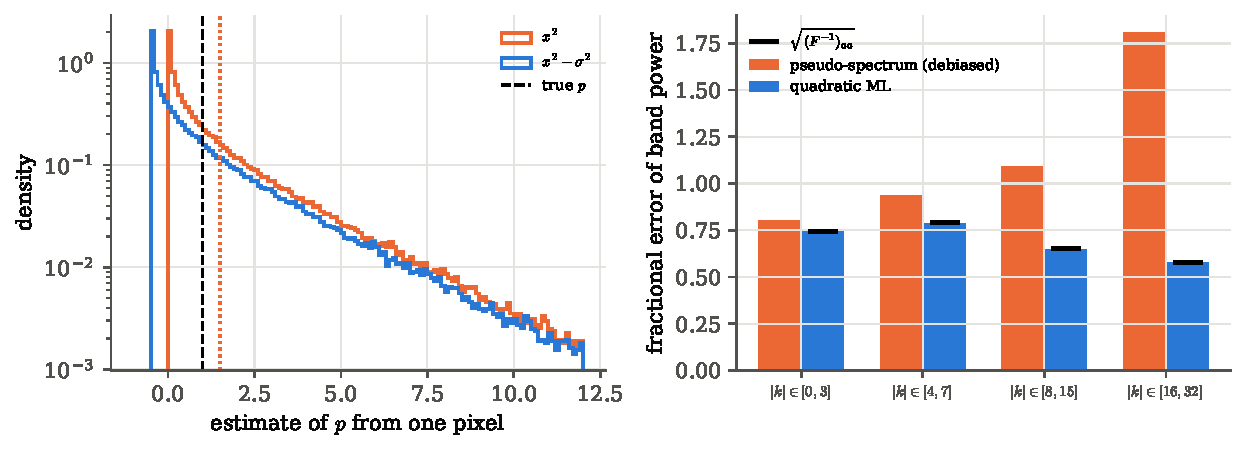
\includegraphics[width=\linewidth]{figures/chT5/quadratic.pdf}
\caption{Left: one pixel with signal variance $p=1$ and noise variance $0.5$.
The square of the reading (orange) is centred on $p+\sigma^2$, not on $p$;
subtracting the noise variance (blue) centres it on $p$ (dashed), but the
spread, set by $p+\sigma^2$, stays. Right: the fractional error of four band
powers of a gapped field with uneven noise, for the debiased pseudo-spectrum
(orange) and the QML estimator (blue); black marks are the Fisher
prediction $\sqrt{(\Fish^{-1})_{aa}}$.}
\label{T5a:fig:quadratic}
\end{figure}

\Cref{T5a:fig:quadratic} (right) shows the result. Both estimators are
unbiased. The QML standard deviations, $\TFiveAQcSdQOne$, $\TFiveAQcSdQTwo$,
$\TFiveAQcSdQThree$ and $\TFiveAQcSdQFour$ for the four bands, match the
Fisher predictions $\TFiveAQcSdThOne$, $\TFiveAQcSdThTwo$, $\TFiveAQcSdThThree$
and $\TFiveAQcSdThFour$. The pseudo-spectrum's variance is larger by factors
$\TFiveAQcVarRatioOne$, $\TFiveAQcVarRatioTwo$, $\TFiveAQcVarRatioThree$ and
$\TFiveAQcVarRatioFour$. The gain grows from band to band because the
higher bands have less signal and are dominated by noise there, and in a
noise-dominated band uniform weights let the shallow, noisy pixels spoil the
estimate, while the QML weights follow the two-pixel example and trust the
deep pixels. In the low bands the signal dominates every pixel, its own
random scatter (cosmic variance) dominates the error, and weighting matters
less.

\begin{inpractice}[Verification versus research]
The Monte Carlo above \emph{verifies} a known result: the QML covariance is
$\Fish^{-1}$, and a simulation that reproduces it tests the code. In real
analyses the roles change. QML needs $\Cmat^{-1}$ for all observed pixels,
an $N^3$ operation, so it is used where $N$ is small: the large angular
scales of a CMB map, degraded to a few thousand pixels, where the mask
couples multipoles most strongly. At high $\ell$ the pseudo-$C_\ell$ method,
with weights chosen per scale (uniform where the signal dominates, inverse
noise where the noise does), recovers most of the QML precision at a tiny
fraction of the cost, and its covariance is calibrated with simulations,
the research instrument when no formula is exact. Hybrid analyses join the
two at an intermediate $\ell$ \cite{Efstathiou2004}.
\end{inpractice}

\subsection{The same structure elsewhere}
\label{T5a:sec:quad-elsewhere}

\emph{Cross-spectra need no noise bias.} If two detectors see the same sky
with independent noises, the product of their readings has mean
$\E(s+n_A)(s+n_B)=\E s^2$: the noise terms average to zero because the two
noises are independent. A quadratic estimator built from products of
\emph{different} detectors therefore has $b=0$, and an error in the noise
model cannot bias it. This is why spectra are often computed from
cross-correlations of data splits (\cref{8a:sec:cross}). The noise still adds
variance, by \eqref{T5a:eq:quad-var}.

\emph{The lensing quadratic estimator.} Gravitational lensing correlates CMB
modes that would otherwise be independent, and the reconstruction of the
lensing potential is a weighted sum of products of pairs of temperature
modes, a quadratic estimator whose weights are chosen, as in
\eqref{T5a:eq:qml-one}, to minimise its noise \cite{HuOkamoto2002}
(\cref{T1b:eq:qe-mv}). Its power spectrum is then \emph{quartic} in the
temperature, and the Gaussian, unlensed part of that four-point function
contributes a constant, the $N_0$ bias (\cref{T1b:eq:n0-general}). It plays
exactly the role of $b$ in \eqref{T5a:eq:trace-condition}: what the
estimator returns from data that contain no lensing at all.

\paragraph{When to use a quadratic estimator.}
Whenever the parameter sets a variance, a power spectrum, a correlation or
a noise level rather than a mean, a quadratic estimator is required, and the
noise bias must be computed (or avoided with cross-correlations). Use QML
when the data set is small enough to invert its covariance and its geometry
is irregular; use pseudo-spectra with simulation-calibrated errors when it is
large; use the plain average of squared modes when the geometry is so
symmetric that the two coincide.

\begin{recap}
\begin{itemize}[itemsep=1pt,leftmargin=1.2em]
  \item An estimator is chosen by answering questions about the problem: what is known about the noise, whether a prior is worth using, whether the parameter lives in the mean or the covariance, how many parameters there are, whether data stream in, and whether the best recipe needs the answer. Same variance, different noise laws: the best estimator of a centre changed by a factor of five.
  \item Gauss--Markov: for $\data=\mathbf A\params+\bm n$ with $\Cov\bm n=\Cmat$, $(\mathbf A\T\Cmat^{-1}\mathbf A)^{-1}\mathbf A\T\Cmat^{-1}\data$ has the smallest covariance among linear unbiased estimators, whatever the noise law; for Gaussian noise it is the best unbiased estimator of all. Nonlinear recipes beat it under heavy tails.
  \item A Bayes estimator lowers the error where the prior is right and raises it where it is wrong: for a Gaussian pull, it wins when $|\theta-\mu_0|<\sqrt{2\tau^2+s^2}$. A constant-risk Bayes estimator is minimax. The linear--Gaussian posterior mean is the Wiener filter (ridge regression), with error $P_sP_n/(P_s+P_n)$ per mode and a fainter, biased map.
  \item Stein: for $k\ge3$ Gaussian means, shrinking all readings by $1-(k-2)/|\bm X|^2$ lowers the total risk for every truth, to $2$ when all means are zero; it is empirical Bayes with the shrinkage estimated from the spread. The guarantee is for the total; one outlying mean can be estimated three times worse.
  \item Robust estimators bound the pull of each reading. Influence function $\psi/\E\psi'$, variance $\E\psi^2/(\E\psi')^2\ge1/I$; Huber's $k=1.345$ costs $5\%$ at the Gaussian and saves an order of magnitude with $10\%$ wild readings; the median breaks down only at one half.
  \item Quadratic estimators $\data\T\mathbf E\data-b$ find parameters in the covariance. Unbiased when $\tr(\mathbf E_a\Cmat_b)=\delta_{ab}$ and $b=\tr(\mathbf E\mathbf N)$; variance $2\tr(\mathbf E\Cmat\mathbf E\Cmat)$ for Gaussian data; the best weights $\Cmat^{-1}\Cmat_a\Cmat^{-1}$ normalised by the Fisher matrix reach $\Fish^{-1}$. For a variance target the noise is a bias as well as a scatter.
\end{itemize}
\end{recap}

\providecommand{\TFiveBTwoSzero}{}\renewcommand{\TFiveBTwoSzero}{11}
\providecommand{\TFiveBTwoSone}{}\renewcommand{\TFiveBTwoSone}{9.444}
\providecommand{\TFiveBTwoStwo}{}\renewcommand{\TFiveBTwoStwo}{9.349}
\providecommand{\TFiveBTwoSthree}{}\renewcommand{\TFiveBTwoSthree}{9.343}
\providecommand{\TFiveBTwoShat}{}\renewcommand{\TFiveBTwoShat}{9.343}
\providecommand{\TFiveBTwoGprime}{}\renewcommand{\TFiveBTwoGprime}{0.06539}
\providecommand{\TFiveBTwoRate}{}\renewcommand{\TFiveBTwoRate}{0.06513}
\providecommand{\TFiveBTwoSney}{}\renewcommand{\TFiveBTwoSney}{9.111}
\providecommand{\TFiveBTwoSigML}{}\renewcommand{\TFiveBTwoSigML}{2.967}
\providecommand{\TFiveBTwoSigEq}{}\renewcommand{\TFiveBTwoSigEq}{3.56}
\providecommand{\TFiveBTwoVarRatio}{}\renewcommand{\TFiveBTwoVarRatio}{0.6948}
\providecommand{\TFiveBBinNbins}{}\renewcommand{\TFiveBBinNbins}{20}
\providecommand{\TFiveBBinNtoys}{}\renewcommand{\TFiveBBinNtoys}{20000}
\providecommand{\TFiveBBinSig}{}\renewcommand{\TFiveBBinSig}{20}
\providecommand{\TFiveBBinBkg}{}\renewcommand{\TFiveBBinBkg}{100}
\providecommand{\TFiveBBinBkgPerBin}{}\renewcommand{\TFiveBBinBkgPerBin}{5}
\providecommand{\TFiveBBinNeyOne}{}\renewcommand{\TFiveBBinNeyOne}{-0.996}
\providecommand{\TFiveBBinPeaOne}{}\renewcommand{\TFiveBBinPeaOne}{0.4381}
\providecommand{\TFiveBBinMLOne}{}\renewcommand{\TFiveBBinMLOne}{0.01409}
\providecommand{\TFiveBBinNeySixteen}{}\renewcommand{\TFiveBBinNeySixteen}{-0.2143}
\providecommand{\TFiveBBinPeaSixteen}{}\renewcommand{\TFiveBBinPeaSixteen}{0.1053}
\providecommand{\TFiveBBinMLSixteen}{}\renewcommand{\TFiveBBinMLSixteen}{-6.637\times10^{-4}}
\providecommand{\TFiveBBinGpOne}{}\renewcommand{\TFiveBBinGpOne}{0.02021}
\providecommand{\TFiveBBinGpNineOne}{}\renewcommand{\TFiveBBinGpNineOne}{0.04999}
\providecommand{\TFiveBBinGpSixteen}{}\renewcommand{\TFiveBBinGpSixteen}{0.004911}
\providecommand{\TFiveBBinMCerr}{}\renewcommand{\TFiveBBinMCerr}{0.007071}
\providecommand{\TFiveBBinCountsLow}{}\renewcommand{\TFiveBBinCountsLow}{1.25}
\providecommand{\TFiveBBinCountsHigh}{}\renewcommand{\TFiveBBinCountsHigh}{160}
\providecommand{\TFiveBBinNeyLow}{}\renewcommand{\TFiveBBinNeyLow}{-1.006}
\providecommand{\TFiveBBinPeaLow}{}\renewcommand{\TFiveBBinPeaLow}{0.8107}
\providecommand{\TFiveBBinMLLow}{}\renewcommand{\TFiveBBinMLLow}{0.002532}
\providecommand{\TFiveBBinNonconvLow}{}\renewcommand{\TFiveBBinNonconvLow}{0.065}
\providecommand{\TFiveBBinNonconvOne}{}\renewcommand{\TFiveBBinNonconvOne}{0}
\providecommand{\TFiveBToyGprime}{}\renewcommand{\TFiveBToyGprime}{0.03062}
\providecommand{\TFiveBHubOne}{}\renewcommand{\TFiveBHubOne}{-4.286\times10^{-4}}
\providecommand{\TFiveBHubTwo}{}\renewcommand{\TFiveBHubTwo}{0.3396}
\providecommand{\TFiveBHubThree}{}\renewcommand{\TFiveBHubThree}{0.6352}
\providecommand{\TFiveBHubFour}{}\renewcommand{\TFiveBHubFour}{0.8574}
\providecommand{\TFiveBHubFive}{}\renewcommand{\TFiveBHubFive}{1.072}
\providecommand{\TFiveBHubSix}{}\renewcommand{\TFiveBHubSix}{1.172}
\providecommand{\TFiveBHubEight}{}\renewcommand{\TFiveBHubEight}{1.338}
\providecommand{\TFiveBHubTen}{}\renewcommand{\TFiveBHubTen}{1.338}
\providecommand{\TFiveBHubMean}{}\renewcommand{\TFiveBHubMean}{1.338}
\providecommand{\TFiveBHubMedian}{}\renewcommand{\TFiveBHubMedian}{-0.21}
\providecommand{\TFiveBHubKzero}{}\renewcommand{\TFiveBHubKzero}{1.5}
\providecommand{\TFiveBHubThetaKzero}{}\renewcommand{\TFiveBHubThetaKzero}{0.1521}
\providecommand{\TFiveBHubGpFormula}{}\renewcommand{\TFiveBHubGpFormula}{0.1064}
\providecommand{\TFiveBHubGpMeas}{}\renewcommand{\TFiveBHubGpMeas}{0.1064}
\providecommand{\TFiveBHubNclip}{}\renewcommand{\TFiveBHubNclip}{3}
\providecommand{\TFiveBHubIters}{}\renewcommand{\TFiveBHubIters}{10}
\providecommand{\TFiveBHubPathZero}{}\renewcommand{\TFiveBHubPathZero}{-0.21}
\providecommand{\TFiveBHubPathOne}{}\renewcommand{\TFiveBHubPathOne}{0.1165}
\providecommand{\TFiveBHubPathTwo}{}\renewcommand{\TFiveBHubPathTwo}{0.1484}
\providecommand{\TFiveBPoiTau}{}\renewcommand{\TFiveBPoiTau}{4}
\providecommand{\TFiveBPoiLamZero}{}\renewcommand{\TFiveBPoiLamZero}{50}
\providecommand{\TFiveBPoiNzero}{}\renewcommand{\TFiveBPoiNzero}{4}
\providecommand{\TFiveBPoiTauIRLS}{}\renewcommand{\TFiveBPoiTauIRLS}{3.922}
\providecommand{\TFiveBPoiTauErr}{}\renewcommand{\TFiveBPoiTauErr}{0.2825}
\providecommand{\TFiveBPoiTauLog}{}\renewcommand{\TFiveBPoiTauLog}{4.537}
\providecommand{\TFiveBPoiIters}{}\renewcommand{\TFiveBPoiIters}{4}
\providecommand{\TFiveBPoiErrOne}{}\renewcommand{\TFiveBPoiErrOne}{0.00221}
\providecommand{\TFiveBPoiErrTwo}{}\renewcommand{\TFiveBPoiErrTwo}{2.268\times10^{-6}}
\providecommand{\TFiveBPoiErrThree}{}\renewcommand{\TFiveBPoiErrThree}{2.225\times10^{-12}}
\providecommand{\TFiveBPoiNtoys}{}\renewcommand{\TFiveBPoiNtoys}{5000}
\providecommand{\TFiveBPoiMeanML}{}\renewcommand{\TFiveBPoiMeanML}{4.006}
\providecommand{\TFiveBPoiSdML}{}\renewcommand{\TFiveBPoiSdML}{0.2948}
\providecommand{\TFiveBPoiMeanLog}{}\renewcommand{\TFiveBPoiMeanLog}{4.485}
\providecommand{\TFiveBPoiSdLog}{}\renewcommand{\TFiveBPoiSdLog}{0.3789}
\providecommand{\TFiveBPoiMeanWlog}{}\renewcommand{\TFiveBPoiMeanWlog}{4.393}
\providecommand{\TFiveBPoiSdWlog}{}\renewcommand{\TFiveBPoiSdWlog}{0.3375}
\providecommand{\TFiveBPoiMCerr}{}\renewcommand{\TFiveBPoiMCerr}{0.004169}
\providecommand{\TFiveBEmN}{}\renewcommand{\TFiveBEmN}{1000}
\providecommand{\TFiveBEmF}{}\renewcommand{\TFiveBEmF}{0.1}
\providecommand{\TFiveBEmMu}{}\renewcommand{\TFiveBEmMu}{125}
\providecommand{\TFiveBEmSig}{}\renewcommand{\TFiveBEmSig}{2}
\providecommand{\TFiveBEmA}{}\renewcommand{\TFiveBEmA}{100}
\providecommand{\TFiveBEmB}{}\renewcommand{\TFiveBEmB}{160}
\providecommand{\TFiveBEmNsig}{}\renewcommand{\TFiveBEmNsig}{97}
\providecommand{\TFiveBEmFhat}{}\renewcommand{\TFiveBEmFhat}{0.1073}
\providecommand{\TFiveBEmFerr}{}\renewcommand{\TFiveBEmFerr}{0.01508}
\providecommand{\TFiveBEmFerrCom}{}\renewcommand{\TFiveBEmFerrCom}{0.009787}
\providecommand{\TFiveBEmRate}{}\renewcommand{\TFiveBEmRate}{0.5791}
\providecommand{\TFiveBEmRateMeas}{}\renewcommand{\TFiveBEmRateMeas}{0.5791}
\providecommand{\TFiveBEmItersA}{}\renewcommand{\TFiveBEmItersA}{38}
\providecommand{\TFiveBEmPathOne}{}\renewcommand{\TFiveBEmPathOne}{0.2146}
\providecommand{\TFiveBEmPathTwo}{}\renewcommand{\TFiveBEmPathTwo}{0.153}
\providecommand{\TFiveBEmPathThree}{}\renewcommand{\TFiveBEmPathThree}{0.1302}
\providecommand{\TFiveBEmBf}{}\renewcommand{\TFiveBEmBf}{0.1043}
\providecommand{\TFiveBEmBmu}{}\renewcommand{\TFiveBEmBmu}{125.3}
\providecommand{\TFiveBEmBsig}{}\renewcommand{\TFiveBEmBsig}{1.811}
\providecommand{\TFiveBEmItersB}{}\renewcommand{\TFiveBEmItersB}{219}
\providecommand{\TFiveBEmBstartLL}{}\renewcommand{\TFiveBEmBstartLL}{-179.7}
\providecommand{\TFiveBEmRateHalf}{}\renewcommand{\TFiveBEmRateHalf}{0.2766}
\providecommand{\TFiveBEmRateTwo}{}\renewcommand{\TFiveBEmRateTwo}{0.5997}
\providecommand{\TFiveBEmRateEight}{}\renewcommand{\TFiveBEmRateEight}{0.9047}
\providecommand{\TFiveBEmRateTwelve}{}\renewcommand{\TFiveBEmRateTwelve}{0.958}
\providecommand{\TFiveBEmMeasTwelve}{}\renewcommand{\TFiveBEmMeasTwelve}{0.9616}
\providecommand{\TFiveBEmMeasHalf}{}\renewcommand{\TFiveBEmMeasHalf}{0.272}
\providecommand{\TFiveBEmStepsTwelve}{}\renewcommand{\TFiveBEmStepsTwelve}{322}
\providecommand{\TFiveBEmStepsHalf}{}\renewcommand{\TFiveBEmStepsHalf}{10.75}
\providecommand{\TFiveBLamBiasPlainFive}{}\renewcommand{\TFiveBLamBiasPlainFive}{0.2462}
\providecommand{\TFiveBLamSdPlainFive}{}\renewcommand{\TFiveBLamSdPlainFive}{0.7151}
\providecommand{\TFiveBLamMsePlainFive}{}\renewcommand{\TFiveBLamMsePlainFive}{0.5719}
\providecommand{\TFiveBLamBiasJKFive}{}\renewcommand{\TFiveBLamBiasJKFive}{-0.08422}
\providecommand{\TFiveBLamSdJKFive}{}\renewcommand{\TFiveBLamSdJKFive}{0.7432}
\providecommand{\TFiveBLamMseJKFive}{}\renewcommand{\TFiveBLamMseJKFive}{0.5594}
\providecommand{\TFiveBLamBiasBootFive}{}\renewcommand{\TFiveBLamBiasBootFive}{-0.0486}
\providecommand{\TFiveBLamSdBootFive}{}\renewcommand{\TFiveBLamSdBootFive}{1.084}
\providecommand{\TFiveBLamMseBootFive}{}\renewcommand{\TFiveBLamMseBootFive}{1.178}
\providecommand{\TFiveBLamBiasParOneFive}{}\renewcommand{\TFiveBLamBiasParOneFive}{-0.06538}
\providecommand{\TFiveBLamSdParOneFive}{}\renewcommand{\TFiveBLamSdParOneFive}{0.5363}
\providecommand{\TFiveBLamMseParOneFive}{}\renewcommand{\TFiveBLamMseParOneFive}{0.2919}
\providecommand{\TFiveBLamBiasParTwoFive}{}\renewcommand{\TFiveBLamBiasParTwoFive}{0.0125}
\providecommand{\TFiveBLamSdParTwoFive}{}\renewcommand{\TFiveBLamSdParTwoFive}{0.581}
\providecommand{\TFiveBLamMseParTwoFive}{}\renewcommand{\TFiveBLamMseParTwoFive}{0.3377}
\providecommand{\TFiveBLamBiasParInfFive}{}\renewcommand{\TFiveBLamBiasParInfFive}{-0.003074}
\providecommand{\TFiveBLamSdParInfFive}{}\renewcommand{\TFiveBLamSdParInfFive}{0.5721}
\providecommand{\TFiveBLamMseParInfFive}{}\renewcommand{\TFiveBLamMseParInfFive}{0.3273}
\providecommand{\TFiveBLamBiasErrFive}{}\renewcommand{\TFiveBLamBiasErrFive}{0.005421}
\providecommand{\TFiveBLamBiasErrJKFive}{}\renewcommand{\TFiveBLamBiasErrJKFive}{0.003716}
\providecommand{\TFiveBLamBiasDbootFive}{}\renewcommand{\TFiveBLamBiasDbootFive}{0.4332}
\providecommand{\TFiveBLamMedDbootFive}{}\renewcommand{\TFiveBLamMedDbootFive}{-0.06696}
\providecommand{\TFiveBLamSdDbootFive}{}\renewcommand{\TFiveBLamSdDbootFive}{25.86}
\providecommand{\TFiveBLamBiasErrDFive}{}\renewcommand{\TFiveBLamBiasErrDFive}{0.1293}
\providecommand{\TFiveBLamIqrDbootFive}{}\renewcommand{\TFiveBLamIqrDbootFive}{0.7191}
\providecommand{\TFiveBLamIqrBootFive}{}\renewcommand{\TFiveBLamIqrBootFive}{0.6066}
\providecommand{\TFiveBLamIqrPlainFive}{}\renewcommand{\TFiveBLamIqrPlainFive}{0.6859}
\providecommand{\TFiveBLamFracBigDbootFive}{}\renewcommand{\TFiveBLamFracBigDbootFive}{3.755}
\providecommand{\TFiveBLamFracBigPlainFive}{}\renewcommand{\TFiveBLamFracBigPlainFive}{2.708}
\providecommand{\TFiveBLamBiasPlainTen}{}\renewcommand{\TFiveBLamBiasPlainTen}{0.1105}
\providecommand{\TFiveBLamSdPlainTen}{}\renewcommand{\TFiveBLamSdPlainTen}{0.3937}
\providecommand{\TFiveBLamMsePlainTen}{}\renewcommand{\TFiveBLamMsePlainTen}{0.1672}
\providecommand{\TFiveBLamBiasJKTen}{}\renewcommand{\TFiveBLamBiasJKTen}{-0.01532}
\providecommand{\TFiveBLamSdJKTen}{}\renewcommand{\TFiveBLamSdJKTen}{0.3633}
\providecommand{\TFiveBLamMseJKTen}{}\renewcommand{\TFiveBLamMseJKTen}{0.1322}
\providecommand{\TFiveBLamBiasBootTen}{}\renewcommand{\TFiveBLamBiasBootTen}{-7.750\times10^{-5}}
\providecommand{\TFiveBLamSdBootTen}{}\renewcommand{\TFiveBLamSdBootTen}{0.3642}
\providecommand{\TFiveBLamMseBootTen}{}\renewcommand{\TFiveBLamMseBootTen}{0.1327}
\providecommand{\TFiveBLamBiasParOneTen}{}\renewcommand{\TFiveBLamBiasParOneTen}{-0.01285}
\providecommand{\TFiveBLamSdParOneTen}{}\renewcommand{\TFiveBLamSdParOneTen}{0.3499}
\providecommand{\TFiveBLamMseParOneTen}{}\renewcommand{\TFiveBLamMseParOneTen}{0.1226}
\providecommand{\TFiveBLamBiasParTwoTen}{}\renewcommand{\TFiveBLamBiasParTwoTen}{8.628\times10^{-4}}
\providecommand{\TFiveBLamSdParTwoTen}{}\renewcommand{\TFiveBLamSdParTwoTen}{0.3548}
\providecommand{\TFiveBLamMseParTwoTen}{}\renewcommand{\TFiveBLamMseParTwoTen}{0.1259}
\providecommand{\TFiveBLamBiasParInfTen}{}\renewcommand{\TFiveBLamBiasParInfTen}{-5.082\times10^{-4}}
\providecommand{\TFiveBLamSdParInfTen}{}\renewcommand{\TFiveBLamSdParInfTen}{0.3543}
\providecommand{\TFiveBLamMseParInfTen}{}\renewcommand{\TFiveBLamMseParInfTen}{0.1255}
\providecommand{\TFiveBLamBiasErrTen}{}\renewcommand{\TFiveBLamBiasErrTen}{0.001821}
\providecommand{\TFiveBLamBiasErrJKTen}{}\renewcommand{\TFiveBLamBiasErrJKTen}{0.001817}
\providecommand{\TFiveBLamBiasDbootTen}{}\renewcommand{\TFiveBLamBiasDbootTen}{0.009755}
\providecommand{\TFiveBLamMedDbootTen}{}\renewcommand{\TFiveBLamMedDbootTen}{-0.06168}
\providecommand{\TFiveBLamSdDbootTen}{}\renewcommand{\TFiveBLamSdDbootTen}{0.3779}
\providecommand{\TFiveBLamBiasErrDTen}{}\renewcommand{\TFiveBLamBiasErrDTen}{0.00189}
\providecommand{\TFiveBLamIqrDbootTen}{}\renewcommand{\TFiveBLamIqrDbootTen}{0.4331}
\providecommand{\TFiveBLamIqrBootTen}{}\renewcommand{\TFiveBLamIqrBootTen}{0.422}
\providecommand{\TFiveBLamIqrPlainTen}{}\renewcommand{\TFiveBLamIqrPlainTen}{0.4559}
\providecommand{\TFiveBLamFracBigDbootTen}{}\renewcommand{\TFiveBLamFracBigDbootTen}{0.175}
\providecommand{\TFiveBLamFracBigPlainTen}{}\renewcommand{\TFiveBLamFracBigPlainTen}{0.275}
\providecommand{\TFiveBLamBiasPlainTwenty}{}\renewcommand{\TFiveBLamBiasPlainTwenty}{0.05284}
\providecommand{\TFiveBLamSdPlainTwenty}{}\renewcommand{\TFiveBLamSdPlainTwenty}{0.2486}
\providecommand{\TFiveBLamMsePlainTwenty}{}\renewcommand{\TFiveBLamMsePlainTwenty}{0.06461}
\providecommand{\TFiveBLamBiasJKTwenty}{}\renewcommand{\TFiveBLamBiasJKTwenty}{-0.002648}
\providecommand{\TFiveBLamSdJKTwenty}{}\renewcommand{\TFiveBLamSdJKTwenty}{0.2372}
\providecommand{\TFiveBLamMseJKTwenty}{}\renewcommand{\TFiveBLamMseJKTwenty}{0.05627}
\providecommand{\TFiveBLamBiasBootTwenty}{}\renewcommand{\TFiveBLamBiasBootTwenty}{0.001663}
\providecommand{\TFiveBLamSdBootTwenty}{}\renewcommand{\TFiveBLamSdBootTwenty}{0.239}
\providecommand{\TFiveBLamMseBootTwenty}{}\renewcommand{\TFiveBLamMseBootTwenty}{0.0571}
\providecommand{\TFiveBLamBiasParOneTwenty}{}\renewcommand{\TFiveBLamBiasParOneTwenty}{-0.002577}
\providecommand{\TFiveBLamSdParOneTwenty}{}\renewcommand{\TFiveBLamSdParOneTwenty}{0.2355}
\providecommand{\TFiveBLamMseParOneTwenty}{}\renewcommand{\TFiveBLamMseParOneTwenty}{0.05549}
\providecommand{\TFiveBLamBiasParTwoTwenty}{}\renewcommand{\TFiveBLamBiasParTwoTwenty}{3.393\times10^{-4}}
\providecommand{\TFiveBLamSdParTwoTwenty}{}\renewcommand{\TFiveBLamSdParTwoTwenty}{0.2362}
\providecommand{\TFiveBLamMseParTwoTwenty}{}\renewcommand{\TFiveBLamMseParTwoTwenty}{0.05581}
\providecommand{\TFiveBLamBiasParInfTwenty}{}\renewcommand{\TFiveBLamBiasParInfTwenty}{1.935\times10^{-4}}
\providecommand{\TFiveBLamSdParInfTwenty}{}\renewcommand{\TFiveBLamSdParInfTwenty}{0.2362}
\providecommand{\TFiveBLamMseParInfTwenty}{}\renewcommand{\TFiveBLamMseParInfTwenty}{0.05579}
\providecommand{\TFiveBLamBiasErrTwenty}{}\renewcommand{\TFiveBLamBiasErrTwenty}{0.001195}
\providecommand{\TFiveBLamBiasErrJKTwenty}{}\renewcommand{\TFiveBLamBiasErrJKTwenty}{0.001186}
\providecommand{\TFiveBLamBiasDbootTwenty}{}\renewcommand{\TFiveBLamBiasDbootTwenty}{0.002267}
\providecommand{\TFiveBLamMedDbootTwenty}{}\renewcommand{\TFiveBLamMedDbootTwenty}{-0.03105}
\providecommand{\TFiveBLamSdDbootTwenty}{}\renewcommand{\TFiveBLamSdDbootTwenty}{0.2433}
\providecommand{\TFiveBLamBiasErrDTwenty}{}\renewcommand{\TFiveBLamBiasErrDTwenty}{0.001216}
\providecommand{\TFiveBLamIqrDbootTwenty}{}\renewcommand{\TFiveBLamIqrDbootTwenty}{0.3035}
\providecommand{\TFiveBLamIqrBootTwenty}{}\renewcommand{\TFiveBLamIqrBootTwenty}{0.2982}
\providecommand{\TFiveBLamIqrPlainTwenty}{}\renewcommand{\TFiveBLamIqrPlainTwenty}{0.3095}
\providecommand{\TFiveBLamFracBigDbootTwenty}{}\renewcommand{\TFiveBLamFracBigDbootTwenty}{0.0075}
\providecommand{\TFiveBLamFracBigPlainTwenty}{}\renewcommand{\TFiveBLamFracBigPlainTwenty}{0.0075}
\providecommand{\TFiveBLamBiasPlainForty}{}\renewcommand{\TFiveBLamBiasPlainForty}{0.02635}
\providecommand{\TFiveBLamSdPlainForty}{}\renewcommand{\TFiveBLamSdPlainForty}{0.1664}
\providecommand{\TFiveBLamMsePlainForty}{}\renewcommand{\TFiveBLamMsePlainForty}{0.02838}
\providecommand{\TFiveBLamBiasJKForty}{}\renewcommand{\TFiveBLamBiasJKForty}{-2.371\times10^{-5}}
\providecommand{\TFiveBLamSdJKForty}{}\renewcommand{\TFiveBLamSdJKForty}{0.1622}
\providecommand{\TFiveBLamMseJKForty}{}\renewcommand{\TFiveBLamMseJKForty}{0.02632}
\providecommand{\TFiveBLamBiasBootForty}{}\renewcommand{\TFiveBLamBiasBootForty}{0.001103}
\providecommand{\TFiveBLamSdBootForty}{}\renewcommand{\TFiveBLamSdBootForty}{0.1633}
\providecommand{\TFiveBLamMseBootForty}{}\renewcommand{\TFiveBLamMseBootForty}{0.02666}
\providecommand{\TFiveBLamBiasParOneForty}{}\renewcommand{\TFiveBLamBiasParOneForty}{3.622\times10^{-5}}
\providecommand{\TFiveBLamSdParOneForty}{}\renewcommand{\TFiveBLamSdParOneForty}{0.1621}
\providecommand{\TFiveBLamMseParOneForty}{}\renewcommand{\TFiveBLamMseParOneForty}{0.02628}
\providecommand{\TFiveBLamBiasParTwoForty}{}\renewcommand{\TFiveBLamBiasParTwoForty}{7.110\times10^{-4}}
\providecommand{\TFiveBLamSdParTwoForty}{}\renewcommand{\TFiveBLamSdParTwoForty}{0.1622}
\providecommand{\TFiveBLamMseParTwoForty}{}\renewcommand{\TFiveBLamMseParTwoForty}{0.02632}
\providecommand{\TFiveBLamBiasParInfForty}{}\renewcommand{\TFiveBLamBiasParInfForty}{6.941\times10^{-4}}
\providecommand{\TFiveBLamSdParInfForty}{}\renewcommand{\TFiveBLamSdParInfForty}{0.1622}
\providecommand{\TFiveBLamMseParInfForty}{}\renewcommand{\TFiveBLamMseParInfForty}{0.02632}
\providecommand{\TFiveBLamBiasErrForty}{}\renewcommand{\TFiveBLamBiasErrForty}{8.164\times10^{-4}}
\providecommand{\TFiveBLamBiasErrJKForty}{}\renewcommand{\TFiveBLamBiasErrJKForty}{8.112\times10^{-4}}
\providecommand{\TFiveBLamNtoys}{}\renewcommand{\TFiveBLamNtoys}{40000}
\providecommand{\TFiveBLamBone}{}\renewcommand{\TFiveBLamBone}{100}
\providecommand{\TFiveBLamBtwo}{}\renewcommand{\TFiveBLamBtwo}{25}
\providecommand{\TFiveBSdPlainBiasFive}{}\renewcommand{\TFiveBSdPlainBiasFive}{-0.0608}
\providecommand{\TFiveBSdPlainVarFive}{}\renewcommand{\TFiveBSdPlainVarFive}{0.1164}
\providecommand{\TFiveBSdPlainMseFive}{}\renewcommand{\TFiveBSdPlainMseFive}{0.1201}
\providecommand{\TFiveBSdJKBiasFive}{}\renewcommand{\TFiveBSdJKBiasFive}{0.01384}
\providecommand{\TFiveBSdJKVarFive}{}\renewcommand{\TFiveBSdJKVarFive}{0.1391}
\providecommand{\TFiveBSdJKMseFive}{}\renewcommand{\TFiveBSdJKMseFive}{0.1393}
\providecommand{\TFiveBSdCfourBiasFive}{}\renewcommand{\TFiveBSdCfourBiasFive}{-8.347\times10^{-4}}
\providecommand{\TFiveBSdCfourVarFive}{}\renewcommand{\TFiveBSdCfourVarFive}{0.1317}
\providecommand{\TFiveBSdCfourMseFive}{}\renewcommand{\TFiveBSdCfourMseFive}{0.1317}
\providecommand{\TFiveBSdPlainBiasTen}{}\renewcommand{\TFiveBSdPlainBiasTen}{-0.02729}
\providecommand{\TFiveBSdPlainVarTen}{}\renewcommand{\TFiveBSdPlainVarTen}{0.05387}
\providecommand{\TFiveBSdPlainMseTen}{}\renewcommand{\TFiveBSdPlainMseTen}{0.05462}
\providecommand{\TFiveBSdJKBiasTen}{}\renewcommand{\TFiveBSdJKBiasTen}{0.002838}
\providecommand{\TFiveBSdJKVarTen}{}\renewcommand{\TFiveBSdJKVarTen}{0.05773}
\providecommand{\TFiveBSdJKMseTen}{}\renewcommand{\TFiveBSdJKMseTen}{0.05774}
\providecommand{\TFiveBSdCfourBiasTen}{}\renewcommand{\TFiveBSdCfourBiasTen}{4.738\times10^{-5}}
\providecommand{\TFiveBSdCfourVarTen}{}\renewcommand{\TFiveBSdCfourVarTen}{0.05695}
\providecommand{\TFiveBSdCfourMseTen}{}\renewcommand{\TFiveBSdCfourMseTen}{0.05695}
\providecommand{\TFiveBSdPlainBiasTwenty}{}\renewcommand{\TFiveBSdPlainBiasTwenty}{-0.01244}
\providecommand{\TFiveBSdPlainVarTwenty}{}\renewcommand{\TFiveBSdPlainVarTwenty}{0.02604}
\providecommand{\TFiveBSdPlainMseTwenty}{}\renewcommand{\TFiveBSdPlainMseTwenty}{0.02619}
\providecommand{\TFiveBSdJKBiasTwenty}{}\renewcommand{\TFiveBSdJKBiasTwenty}{0.001236}
\providecommand{\TFiveBSdJKVarTwenty}{}\renewcommand{\TFiveBSdJKVarTwenty}{0.02681}
\providecommand{\TFiveBSdJKMseTwenty}{}\renewcommand{\TFiveBSdJKMseTwenty}{0.02682}
\providecommand{\TFiveBSdCfourBiasTwenty}{}\renewcommand{\TFiveBSdCfourBiasTwenty}{6.344\times10^{-4}}
\providecommand{\TFiveBSdCfourVarTwenty}{}\renewcommand{\TFiveBSdCfourVarTwenty}{0.02673}
\providecommand{\TFiveBSdCfourMseTwenty}{}\renewcommand{\TFiveBSdCfourMseTwenty}{0.02673}
\providecommand{\TFiveBSdNtoys}{}\renewcommand{\TFiveBSdNtoys}{200000}
\providecommand{\TFiveBCfourFive}{}\renewcommand{\TFiveBCfourFive}{0.94}
\providecommand{\TFiveBCfourTen}{}\renewcommand{\TFiveBCfourTen}{0.9727}
\providecommand{\TFiveBAvgKcross}{}\renewcommand{\TFiveBAvgKcross}{12.68}
\providecommand{\TFiveBAvgRmsPlainHundred}{}\renewcommand{\TFiveBAvgRmsPlainHundred}{0.1176}
\providecommand{\TFiveBAvgRmsJKHundred}{}\renewcommand{\TFiveBAvgRmsJKHundred}{0.04017}
\providecommand{\TFiveBAvgRmsBootHundred}{}\renewcommand{\TFiveBAvgRmsBootHundred}{0.03731}
\providecommand{\TFiveBAvgRmsDbootHundred}{}\renewcommand{\TFiveBAvgRmsDbootHundred}{0.04004}
\providecommand{\TFiveBAvgK}{}\renewcommand{\TFiveBAvgK}{100}
\providecommand{\TFiveBWelN}{}\renewcommand{\TFiveBWelN}{100000}
\providecommand{\TFiveBWelVar}{}\renewcommand{\TFiveBWelVar}{1.0000116}
\providecommand{\TFiveBWelTwo}{}\renewcommand{\TFiveBWelTwo}{1.0000116}
\providecommand{\TFiveBWelNaive}{}\renewcommand{\TFiveBWelNaive}{21140}
\providecommand{\TFiveBWelMeanDiff}{}\renewcommand{\TFiveBWelMeanDiff}{5.007\times10^{-6}}
\providecommand{\TFiveBWelErr}{}\renewcommand{\TFiveBWelErr}{3.213\times10^{-8}}
\providecommand{\TFiveBWelErrNaive}{}\renewcommand{\TFiveBWelErrNaive}{21138}
\providecommand{\TFiveBRlsN}{}\renewcommand{\TFiveBRlsN}{200}
\providecommand{\TFiveBRlsMaxDiff}{}\renewcommand{\TFiveBRlsMaxDiff}{2.748\times10^{-14}}
\providecommand{\TFiveBRlsA}{}\renewcommand{\TFiveBRlsA}{0.4778}
\providecommand{\TFiveBRlsB}{}\renewcommand{\TFiveBRlsB}{1.999}
\providecommand{\TFiveBKfRunDiff}{}\renewcommand{\TFiveBKfRunDiff}{4.663\times10^{-15}}
\providecommand{\TFiveBKfT}{}\renewcommand{\TFiveBKfT}{5000}
\providecommand{\TFiveBKfR}{}\renewcommand{\TFiveBKfR}{200}
\providecommand{\TFiveBKfSq}{}\renewcommand{\TFiveBKfSq}{0.002}
\providecommand{\TFiveBKfSr}{}\renewcommand{\TFiveBKfSr}{0.05}
\providecommand{\TFiveBKfBurn}{}\renewcommand{\TFiveBKfBurn}{500}
\providecommand{\TFiveBKfRms}{}\renewcommand{\TFiveBKfRms}{0.009867}
\providecommand{\TFiveBKfPss}{}\renewcommand{\TFiveBKfPss}{0.009901}
\providecommand{\TFiveBKfKss}{}\renewcommand{\TFiveBKfKss}{0.03921}
\providecommand{\TFiveBKfMem}{}\renewcommand{\TFiveBKfMem}{25.5}
\providecommand{\TFiveBKfRmsRun}{}\renewcommand{\TFiveBKfRmsRun}{0.06061}
\providecommand{\TFiveBKfWbest}{}\renewcommand{\TFiveBKfWbest}{42}
\providecommand{\TFiveBKfRmsWbest}{}\renewcommand{\TFiveBKfRmsWbest}{0.01064}
\providecommand{\TFiveBKfWtheory}{}\renewcommand{\TFiveBKfWtheory}{43.3}
\providecommand{\TFiveBKfRmsWtheory}{}\renewcommand{\TFiveBKfRmsWtheory}{0.01075}
\providecommand{\TFiveBKfWinFrac}{}\renewcommand{\TFiveBKfWinFrac}{100}
\providecommand{\TFiveBKfGain}{}\renewcommand{\TFiveBKfGain}{7.238}
\providecommand{\TFiveBKfRmsQtenth}{}\renewcommand{\TFiveBKfRmsQtenth}{0.01308}
\providecommand{\TFiveBKfRmsQten}{}\renewcommand{\TFiveBKfRmsQten}{0.01308}
\providecommand{\TFiveBKfRmsQhundredth}{}\renewcommand{\TFiveBKfRmsQhundredth}{0.0225}
\providecommand{\TFiveBKfRmsQhundred}{}\renewcommand{\TFiveBKfRmsQhundred}{0.02219}
 
\section{Iteration: solving the equation that defines an estimator}
\label{T5b:sec:iterative}

\paragraph{What we already have.}
Most estimators met so far are formulas. Put the readings in, get the
number out. The weighted mean multiplies each reading by the inverse of its
variance (\cref{3a:sec:weighted}); least squares solves one set of linear
equations, the normal equations (\cref{3b:sec:least-squares}); the best
linear unbiased estimator of \cref{T5a:sec:blue} is a fixed matrix times
the data. Behind every one of these formulas stands an equation. The
maximum-likelihood estimate is the value at which the score vanishes; the
least-squares estimate is the value at which the $\chi^2$ is smallest; the
weighted mean is the value at which the weighted residuals sum to zero.
For these the equation could be solved with algebra, and the solution,
written out, is the formula.

\paragraph{When that is not enough.}
Often the equation that defines the estimate cannot be solved with algebra.
The score of a likelihood may be a sum of nonlinear terms whose root has no
closed form; an estimate may need the inverse of a function that cannot be
inverted on paper; or the unknown may appear on both sides of the equation.
The last case is common with counts: the variance of a Poisson count equals
its mean, so the inverse-variance weights that the best combination needs
contain the very rates we are trying to measure. In all these cases the
estimator is still perfectly well defined: it is the solution of its
equation. What is missing is only a way to compute that solution, and the
standard way is to repeat a simple step until the answer stops changing.
That repetition is what \newterm{iteration} means here. It is a numerical
method for solving an equation, not a new kind of estimator.

\paragraph{A story with the whole trick in it.}
What number squares to two? The question defines the number completely, but
no finite piece of arithmetic produces it. So we guess, and improve the
guess. If $x$ is too large, $2/x$ is too small, and their average is closer
than either: $x_{k+1}=\frac12(x_k+2/x_k)$. Starting from $1$ this gives
$1.5$, then $1.41667$, then $1.414216$, then $1.41421356$, and the next pass
changes nothing in the digits shown. The answer is $\sqrt2$ because $\sqrt2$
is the solution of $x^2=2$, not because of the particular recipe: halving an
interval that brackets the root reaches the same number more slowly, and any
route that converges arrives at the same place. Three things can still go
wrong, and each depends on the route. Stop after two passes and the answer is
$1.41667$, a different number from $\sqrt2$. Start from $-1$ and the same
recipe walks to $-\sqrt2$, the other solution of the same equation. And
rewrite the equation as $x=2/x$ and repeat that step: from $1$ it jumps to $2$,
back to $1$, and on forever, because each correction overshoots the error
it corrects.

Estimators that need iteration are this story with data in it. The
equation is the statistical choice: which equation we write decides the
bias and the scatter of the estimate. The iteration only solves it.
Newton--Raphson for a score equation, Fisher scoring, iteratively reweighted
least squares and the expectation--maximisation algorithm are all recipes
like the averaging step, each a different way of improving a guess. The three ways the
square-root recipe can fail return as the three places where the route does
matter for statistics: stopping early, several solutions, and a step that
overshoots.

\paragraph{The story in symbols: two detectors, one source.}
Each detector counts for the same time and sees the same source, which
contributes on average $s$ counts to each. The backgrounds are known from
observations away from the source: on average $b_1=30$ counts in the first
detector and $b_2=2$ in the second. The detectors record $n_1=44$ and
$n_2=10$. Subtracting the backgrounds gives two readings of $s$,
\[
  x_1=n_1-b_1=14,\qquad x_2=n_2-b_2=8,
\]
each unbiased, $\E x_i=s$, because $\E n_i=s+b_i$. Their variances are those
of the counts, and for a Poisson count the variance equals the mean:
$\Var x_i=s+b_i$. Combining the readings with weights $w_i$ that add up to
one, $\hat s=w_1x_1+w_2x_2$, the variance is smallest for
$w_i\propto1/\Var x_i$ (\cref{3a:eq:wmean-weights}), so
\begin{equation}
  \hat s\eqby{1}\frac{\sum_i x_i/(s+b_i)}{\sum_i 1/(s+b_i)},\qquad
  \Var\hat s\eqby{2}\frac{1}{\sum_i 1/(s+b_i)} .
  \label{T5b:eq:two-det}
\end{equation}
\begin{explain}
  \item Inverse-variance weights $w_i\propto1/(s+b_i)$, divided by their sum
        so that they add up to one.
  \item The variance of the inverse-variance weighted mean is one over the sum
        of the inverse variances \eqref{3a:eq:wmean-weights}.
\end{explain}
The weights contain $s$. That is the dial we have to set, and there are three
obvious ways to set it.

\emph{Ignore the difference between the detectors.} Equal weights give
$\hat s=(14+8)/2=\TFiveBTwoSzero$. Its variance is
$\tfrac14[(s+b_1)+(s+b_2)]$, which at the value we will end up with is
$\TFiveBTwoSigEq^2$: the clean second detector is diluted by the noisy first.

\emph{Take the variances from the data.} The observed counts are estimates of
$s+b_i$, so put $w_i\propto1/n_i$. This gives
$\hat s=(14/44+8/10)/(1/44+1/10)=\TFiveBTwoSney$. It looks harmless but it is
not: a detector whose count fluctuated low is given a small variance and
hence a large weight, so the estimate is pulled towards readings that
fluctuated low. This is the Neyman $\chi^2$ of \cref{3b:sec:neyman-pearson}
in disguise, and \cref{T5b:sec:fixed-ml} measures its bias.

\emph{Use the current answer in the weights, and repeat.} Start from the equal-weight
value, $s_0=\TFiveBTwoSzero$, and compute the weights it implies:
\begin{align}
  s_1&\eqby{1}\frac{14/(11+30)+8/(11+2)}{1/(11+30)+1/(11+2)}
      =\frac{0.34146+0.61538}{0.02439+0.07692}
      \eqby{2}\TFiveBTwoSone,\nonumber\\
  s_2&\eqby{3}\frac{14/(\TFiveBTwoSone+30)+8/(\TFiveBTwoSone+2)}{1/(\TFiveBTwoSone+30)+1/(\TFiveBTwoSone+2)}
      =\TFiveBTwoStwo,\qquad
  s_3=\TFiveBTwoSthree .
  \label{T5b:eq:two-det-iter}
\end{align}
\begin{explain}
  \item \eqref{T5b:eq:two-det} with $s=s_0=11$ in the weights.
  \item Divide: $0.95684/0.10131$.
  \item The same with the new value in the weights; $s_3$ likewise.
\end{explain}
After three passes the value no longer moves in the third decimal. The
value that reproduces itself is $\hat s=\TFiveBTwoShat$, with standard error
$\sqrt{1/\sum_i1/(\hat s+b_i)}=\TFiveBTwoSigML$. Against equal weights the
variance has dropped to $\TFiveBTwoVarRatio$ of its value, as if we had
collected almost half as much data again, and the cost was three more lines
of arithmetic. The weights contain the unknown, so the estimate is the solution
of an equation with $s$ on both sides, $s=g(s)$; feeding each answer back into
the weights is the square-root recipe applied to that equation.

\paragraph{What the iteration decides, and what it does not.}
If the iteration converges, the answer is the solution of the equation, and
which numerical route led there does not matter. Three situations make the
route matter all the same. \emph{Stopping early}: an iteration halted before
it converges returns something that is not the solution of the equation,
and the number of passes becomes part of the estimator, a dial that trades
bias for scatter (\cref{T5b:sec:early-stop}). \emph{Several solutions, or
none that the iteration can reach}: when the equation has more than one root,
as the likelihood of a mixture often does, the starting point decides which
one we get (\cref{T5b:sec:em}), and when the step overshoots, the iteration
never settles at all (\cref{T5b:sec:contraction}). \emph{The choice of
equation}: weights taken from the data, weights taken from the model and
minimised directly, and weights re-solved from the current answer are three
different equations, hence three different estimators with different biases
(\cref{T5b:sec:fixed-ml}); the iteration only solves whichever equation we
chose, and choosing it is the statistical decision. None of this is the same
as updating an estimate when new readings arrive, which consumes new data
instead of reusing the same data; that is the recursion of
\cref{T5b:sec:recursive}.

\paragraph{A picture: the iteration as a staircase.}
Write one pass of the recipe as a function, $s_{k+1}=g(s_k)$, where $g$ is the
right-hand side of \eqref{T5b:eq:two-det} with $s_k$ in the weights. Plot
$g$ against the diagonal line $y=s$ (\cref{T5b:fig:cobweb}). A value that
reproduces itself, $g(s^*)=s^*$, is a point where the curve crosses the
diagonal. The iteration has a simple geometric form. From $s_k$ go up to the
curve to read off $g(s_k)$; go across to the diagonal to make that the new
$s$; go up to the curve again. When the curve is flatter than the diagonal
where they cross, each step lands closer, and the path is a staircase or a
spiral that closes in on the crossing. When the curve is steeper than the
diagonal, each step overshoots more than the last, as the over-reacting
shower did, and the path spirals out. For the two detectors the curve is
almost flat: one step already lands nearly on the crossing.

\begin{figure}[htbp]
\centering
\begin{tikzpicture}
\pgfplotsset{cobweb/.style={width=4.5cm,height=4.5cm,tick label style={font=\scriptsize},label style={font=\small},title style={font=\small}}}
\begin{axis}[cobweb,at={(0,0)},xmin=6,xmax=13,ymin=6,ymax=13,xlabel={$s_k$},ylabel={$s_{k+1}=g(s_k)$},
  title={(a) two detectors}]
  \addplot[faint,domain=6:13] {x};
  \addplot[very thick,formblue,domain=6:13,samples=80]
     {(14/(x+30)+8/(x+2))/(1/(x+30)+1/(x+2))};
  \addplot[thick,fibreorange] coordinates {(11,11) (11,9.4444) (9.4444,9.4444) (9.4444,9.3493) (9.3493,9.3493)};
  \addplot[only marks,mark=*,mark size=1.6pt] coordinates {(11,11)};
  \node[font=\scriptsize,anchor=south west] at (axis cs:11.05,11.05) {$s_0$};
  \node[font=\scriptsize,anchor=north west] at (axis cs:9.6,9.1) {$\hat s$};
\end{axis}
\begin{axis}[cobweb,at={(4.75cm,0)},xmin=0.2,xmax=2.6,ymin=0.2,ymax=2.6,xlabel={$\theta_k$},
  title={(b) slope $0.7$: staircase}]
  \addplot[faint,domain=0.2:2.6] {x};
  \addplot[very thick,formblue,domain=0.2:2.6] {2+0.7*(x-2)};
  \addplot[thick,fibreorange] coordinates {(0.4,0.4) (0.4,0.88) (0.88,0.88) (0.88,1.216) (1.216,1.216)
     (1.216,1.4512) (1.4512,1.4512) (1.4512,1.6158) (1.6158,1.6158) (1.6158,1.7311) (1.7311,1.7311)};
  \addplot[only marks,mark=*,mark size=1.6pt] coordinates {(0.4,0.4)};
  \node[font=\scriptsize,anchor=north west] at (axis cs:0.42,0.38) {$\theta_0$};
\end{axis}
\begin{axis}[cobweb,at={(9.5cm,0)},xmin=1.2,xmax=2.8,ymin=1.2,ymax=2.8,xlabel={$\theta_k$},
  title={(c) slope $-1.25$: spiral out}]
  \addplot[faint,domain=1.2:2.8] {x};
  \addplot[very thick,formblue,domain=1.36:2.64] {2-1.25*(x-2)};
  \addplot[thick,bdryred] coordinates {(1.8,1.8) (1.8,2.25) (2.25,2.25) (2.25,1.6875) (1.6875,1.6875)
     (1.6875,2.3906) (2.3906,2.3906) (2.3906,1.5117) (1.5117,1.5117)};
  \addplot[only marks,mark=*,mark size=1.6pt] coordinates {(1.8,1.8)};
  \node[font=\scriptsize,anchor=north west] at (axis cs:1.82,1.78) {$\theta_0$};
\end{axis}
\end{tikzpicture}
\caption{Fixed-point iteration drawn as a path between the curve $g$ (blue)
and the diagonal (grey). (a) The two-detector recipe: the curve is almost
flat, so from $s_0=11$ the first step lands at $9.444$ and the second at
$9.349$, already on top of the crossing at $\hat s=9.343$. (b) A curve with
slope $0.7$ at the crossing: every step removes $30\%$ of the remaining
error, a staircase that creeps up. (c) A curve with slope $-1.25$: every step
overshoots by more than the last, and the path spirals away from the
crossing.}
\label{T5b:fig:cobweb}
\end{figure}

\paragraph{One idea, many names.}
Finding a value that reproduces itself under a recipe is called
\newterm{fixed-point iteration}, and physics is full of it. In the
Hartree method of atomic physics, each electron moves in the average field
of all the others, but that field depends on the orbitals one is trying to
find: guess the orbitals, compute the field, solve for new orbitals, repeat
until they agree with the field they produce, the \emph{self-consistent
field}. In the mean-field theory of a magnet, the magnetisation sets the
field that sets the magnetisation, $m=\tanh(\beta Jzm)$, and the equation is
solved the same way. In statistics the same idea goes under several names.
When the reweighting is done in a least-squares fit, it is called
iteratively reweighted least squares. When the unknowns are hidden labels,
such as which event was signal, it is the expectation--maximisation (EM)
algorithm. In astronomy, sharpening a blurred image this way is
Richardson--Lucy deconvolution \cite{Richardson1972,Lucy1974}. In particle
physics, undoing a detector's smearing this way is iterative Bayesian
unfolding (\cref{6b:sec:unf-bayes}). Newton--Raphson is also a fixed-point
iteration, with a particularly good choice of $g$. The common language is
calculus on a single function $g$, because convergence is decided by its
slope.

The questions to answer are those the shower already posed. When does the
iteration settle, and how fast (\cref{T5b:sec:contraction})? Is the value
it settles on a good estimator, and in particular is it the maximum
likelihood estimate (\cref{T5b:sec:fixed-ml})? Then come the two most common
forms, reweighted least squares (\cref{T5b:sec:irls}) and EM
(\cref{T5b:sec:em}), and the observation that stopping an iteration early can
be useful in its own right (\cref{T5b:sec:early-stop}).

\subsection{When does the iteration settle, and how fast?}
\label{T5b:sec:contraction}

Let $g$ be the recipe that turns a guess $\theta_k$ into the next guess,
$\theta_{k+1}=g(\theta_k)$, and let $\theta^*$ be a value it reproduces,
$g(\theta^*)=\theta^*$. In the two-detector example $\theta$ is the source
strength $s$ and $g$ is the weighted mean \eqref{T5b:eq:two-det} with the
current guess in the weights. How does the error $e_k=\theta_k-\theta^*$ change
from one pass to the next?
\begin{align}
  e_{k+1}&\eqby{1}g(\theta_k)-g(\theta^*)
         \eqby{2}g'(\xi_k)\,(\theta_k-\theta^*)
         =g'(\xi_k)\,e_k,\nonumber\\
  e_{k+1}&\eqby{3}g'(\theta^*)\,e_k+\tfrac12g''(\theta^*)\,e_k^2+\dots
  \label{T5b:eq:error-map}
\end{align}
\begin{explain}
  \item $\theta_{k+1}=g(\theta_k)$ by definition, and $\theta^*=g(\theta^*)$
        because $\theta^*$ is a fixed point.
  \item The mean value theorem: between any two points the chord of a
        smooth function has the slope of the function at some point $\xi_k$
        in between.
  \item Taylor expansion of $g(\theta_k)$ about $\theta^*$, with
        $g(\theta^*)=\theta^*$ subtracted.
\end{explain}
The first line gives the global statement. If on some interval around
$\theta^*$ the slope obeys $|g'|\le L<1$, and the iteration starts inside that
interval, every pass multiplies the error by at most $L$:
$|e_k|\le L^k|e_0|\to0$. The second line gives the speed once we are close.
The error is multiplied at each pass by the number $g'(\theta^*)$, so
$|e_k|\approx|g'(\theta^*)|^k\,|e_0|$, a straight line on a logarithmic plot.
To gain $d$ decimal digits takes about $d/\log_{10}(1/|g'(\theta^*)|)$ passes:
one pass per digit for $|g'|=0.1$, seven for $|g'|=0.7$, and $230$ for
$|g'|=0.99$. The sign of $g'$ decides the shape of the path: positive gives the
one-sided staircase of \cref{T5b:fig:cobweb}b, negative an error that
changes sign at every pass. And if $|g'(\theta^*)|>1$ the error grows, the
fixed point repels, and no starting point near it converges to it
(\cref{T5b:fig:cobweb}c).

\begin{workdef}[fixed-point iteration and its contraction factor]
A \newterm{fixed-point iteration} repeats $\theta_{k+1}=g(\theta_k)$ until
$\theta$ stops changing. Its \newterm{contraction factor} is
$|g'(\theta^*)|$ \unpack{the fraction of the remaining error that survives
one pass, near the fixed point}. Below one the iteration converges
linearly, gaining a decimal digit every $1/\log_{10}(1/|g'|)$ passes. Above one it
does not converge to $\theta^*$. \emph{Operationally:} record
$|\theta_{k+1}-\theta_k|$; near convergence the ratio of successive changes
is the contraction factor.
\end{workdef}

\emph{Newton's method is a fixed-point iteration with zero slope.} The
Newton--Raphson map of \eqref{3b:eq:newton} is $g(\theta)=\theta-\ell'(\theta)/\ell''(\theta)$,
with $\ell$ the log-likelihood. Its slope at the maximum is
\begin{equation}
  g'(\theta)\eqby{1}1-\frac{\ell''\,\ell''-\ell'\,\ell'''}{(\ell'')^2}
  =\frac{\ell'(\theta)\,\ell'''(\theta)}{\ell''(\theta)^2}
  \eqby{2}0\quad\text{at }\theta=\hat\theta .
  \label{T5b:eq:newton-slope}
\end{equation}
\begin{explain}
  \item Quotient rule for $\ell'/\ell''$: the derivative is
        $(\ell''\ell''-\ell'\ell''')/(\ell'')^2$.
  \item At the maximum the score vanishes, $\ell'(\hat\theta)=0$.
\end{explain}
With $g'(\theta^*)=0$ the first term of \eqref{T5b:eq:error-map} disappears, and
$e_{k+1}\approx\frac12g''(\theta^*)\,e_k^2$: each error is proportional to the
square of the previous one, so the number of correct digits roughly
doubles per pass. That is the behaviour seen in the lifetime example of
\cref{3b:sec:newton}, with errors $0.057$, $0.0052$, $0.00005$. A recipe whose
slope at the fixed point is merely small converges linearly, but fast; a
recipe whose slope there is zero converges quadratically.

\emph{The slope of a reweighting recipe.} Many iterative estimators are
weighted means whose weights depend on the current guess,
$g(\theta)=\sum_iw_i(\theta)x_i/\sum_iw_i(\theta)$. Their slope at the fixed point
has a useful form:
\begin{align}
  g'(\theta)&\eqby{1}\frac{\sum_iw_i'x_i\,\sum_jw_j-\sum_iw_ix_i\,\sum_jw_j'}{\bigl(\sum_jw_j\bigr)^2}
             =\frac{\sum_iw_i'\,\bigl(x_i-g(\theta)\bigr)}{\sum_jw_j},\nonumber\\
  g'(\theta^*)&\eqby{2}\frac{\sum_iw_i'(\theta^*)\,(x_i-\theta^*)}{\sum_jw_j(\theta^*)} .
  \label{T5b:eq:reweight-slope}
\end{align}
\begin{explain}
  \item Quotient rule, with $w_i'=\dd w_i/\dd\theta$; then divide numerator and
        denominator by $\sum_jw_j$ and recognise $g(\theta)=\sum_iw_ix_i/\sum_jw_j$
        in the second term.
  \item At the fixed point $g(\theta^*)=\theta^*$.
\end{explain}
So the slope is a weighted sum of the residuals $x_i-\theta^*$, weighted by how
fast each weight changes. For the two detectors $w_i=1/(s+b_i)$, so
$w_i'=-w_i^2$, and with $\hat s+b_1=39.343$, $\hat s+b_2=11.343$,
\begin{equation}
  g'(\hat s)\eqby{1}-\frac{\sum_iw_i^2(x_i-\hat s)}{\sum_iw_i}
  \eqby{2}-\frac{4.657/39.343^2-1.343/11.343^2}{1/39.343+1/11.343}
  \eqby{3}\TFiveBTwoGprime .
  \label{T5b:eq:two-det-slope}
\end{equation}
\begin{explain}
  \item \eqref{T5b:eq:reweight-slope} with $w_i'=-w_i^2$.
  \item The residuals are $x_1-\hat s=14-9.343=4.657$ and $x_2-\hat s=8-9.343=-1.343$.
  \item The numerator is $0.003009-0.010439=-0.007430$ and the denominator
        $0.11358$.
\end{explain}
Each pass keeps about $6.5\%$ of the remaining error, and the ratio of
successive errors in the run of \pyname{20_iterative_weights.py} is
$\TFiveBTwoRate$: a new correct digit at every pass, as in
\eqref{T5b:eq:two-det-iter}. Why is the slope so small? At the fixed point
the weighted residuals cancel exactly, $\sum_iw_i(x_i-\hat s)=0$, because
$\hat s$ is their weighted mean. The slope weights the same residuals by
$w_i^2$ instead of $w_i$, so only the \emph{difference} in weights between
readings that fell high and readings that fell low survives. Residuals are
noise, of random sign. When the model fits the data, reweighting recipes of
this kind converge in a handful of passes.

\paragraph{When it does not.}
The binned fit of \cref{T5b:sec:fixed-ml} below repeats the same recipe for a
peak of known shape on a flat background, in $\TFiveBBinNtoys$ simulated
spectra at each of several exposures. With $\TFiveBBinBkgPerBin$ background
counts per bin the median contraction factor is $\TFiveBBinGpOne$, and nine
spectra in ten have it below $\TFiveBBinGpNineOne$. At the lowest exposure,
$\TFiveBBinCountsLow$ background counts per bin, a few spectra are so sparse
that the fitted peak sits near the edge of the allowed region, where a
small change of the guess changes the weights of the nearly empty bins a
lot. In $\TFiveBBinNonconvLow\%$ of them the iteration had not converged
after sixty passes, and every one of those had $|g'(\theta^*)|$ above $0.99$,
while every spectrum that converged had it below one. The condition
$|g'|<1$ is not a formality.

\subsection{Where does it settle? At the maximum of the likelihood}
\label{T5b:sec:fixed-ml}

A fixed point is a value that reproduces itself, but nothing so far says it
is a \emph{good} value. For the two detectors we can find out what it is by
writing out the equation it satisfies. Setting $s_{k+1}=s_k=\hat s$ in
\eqref{T5b:eq:two-det} and clearing the denominator,
\begin{equation}
  \sum_i\frac{x_i-\hat s}{\hat s+b_i}\eqby{1}0
  \quad\Longleftrightarrow\quad
  \sum_i\frac{n_i-(\hat s+b_i)}{\hat s+b_i}\eqby{2}0
  \quad\Longleftrightarrow\quad
  \sum_i\Bigl(\frac{n_i}{\hat s+b_i}-1\Bigr)\eqby{3}0 .
  \label{T5b:eq:two-det-fixed}
\end{equation}
\begin{explain}
  \item Multiply $\hat s\sum_i1/(\hat s+b_i)=\sum_ix_i/(\hat s+b_i)$ out and move
        everything to one side.
  \item $x_i=n_i-b_i$.
  \item Split the fraction.
\end{explain}
Now ask a different question: what is the maximum-likelihood estimate of $s$?
The counts are independent Poisson variables with means $s+b_i$, so the
log-likelihood and its derivative, the score, are
\begin{equation}
  \ell(s)\eqby{1}\sum_i\bigl[n_i\ln(s+b_i)-(s+b_i)-\ln n_i!\bigr],
  \qquad
  \ell'(s)\eqby{2}\sum_i\Bigl(\frac{n_i}{s+b_i}-1\Bigr).
  \label{T5b:eq:two-det-score}
\end{equation}
\begin{explain}
  \item The logarithm of the product of Poisson probabilities
        $(s+b_i)^{n_i}e^{-(s+b_i)}/n_i!$.
  \item Differentiate term by term; the factorials do not depend on $s$.
\end{explain}
The score equation $\ell'(\hat s)=0$ is the last form of
\eqref{T5b:eq:two-det-fixed}. So the self-consistent weighted mean is the
maximum-likelihood estimate, which the script confirms by solving the score
equation directly: the two agree to $10^{-10}$. This explains why the iterated
weights beat the two shortcuts. The equal-weight mean ignores what we know
about the noise. The data-weighted mean uses the noise of the data to set
its own weights. The iterated mean is maximum likelihood, efficient for
large samples (\cref{3b:sec:cramer-rao}), reached through a sequence of
weighted averages.

The equivalence is not special to two detectors. Let counts $y_i$ have Poisson
means $\lambda_i(\theta)$, any smooth functions of the parameter. A weighted least
squares fit with weights frozen at the current guess, $\sigma_i^2=\lambda_i(\theta_k)$,
minimises $\sum_i(y_i-\lambda_i(\theta))^2/\lambda_i(\theta_k)$, and its stationarity
condition, evaluated at a fixed point $\theta_k=\theta$, is compared below with
the Poisson score:
\begin{align}
  -\frac12\frac{\partial}{\partial\theta}\sum_i\frac{(y_i-\lambda_i(\theta))^2}{\lambda_i(\theta_k)}
  \Big|_{\theta_k=\theta}
  &\eqby{1}\sum_i\frac{y_i-\lambda_i(\theta)}{\lambda_i(\theta)}\,\frac{\partial\lambda_i}{\partial\theta},\nonumber\\
  \frac{\partial}{\partial\theta}\sum_i\bigl[y_i\ln\lambda_i(\theta)-\lambda_i(\theta)\bigr]
  &\eqby{2}\sum_i\Bigl(\frac{y_i}{\lambda_i}-1\Bigr)\frac{\partial\lambda_i}{\partial\theta}
   =\sum_i\frac{y_i-\lambda_i}{\lambda_i}\,\frac{\partial\lambda_i}{\partial\theta}.
  \label{T5b:eq:poisson-irls}
\end{align}
\begin{explain}
  \item Only the numerator depends on $\theta$ when the weights are frozen;
        the chain rule gives $-2(y_i-\lambda_i)\,\partial\lambda_i/\partial\theta$.
        Then set the frozen value equal to the current one.
  \item The Poisson log-likelihood without its $\theta$-free term $-\ln y_i!$,
        differentiated by the chain rule.
\end{explain}
The two right-hand sides are identical.

\begin{keyidea}[Re-solved weights land on the score equation]
For counts whose variance equals their mean, a least-squares fit whose
weights $1/\lambda_i(\theta)$ are recomputed from the current fit and the fit
repeated until nothing changes converges, if it converges, to the root of
the Poisson score: the maximum-likelihood estimate. Neither weights from the
data, $1/y_i$, nor weights from the model differentiated along with the
residuals have this property.
\end{keyidea}

\paragraph{The two shortcuts, met again.}
\Cref{3b:sec:neyman-pearson} fitted the normalisation of a histogram in two
popular ways. The Neyman $\chi^2$ takes each bin's variance from the data,
$\sum_i(y_i-\lambda_i)^2/y_i$. The Pearson $\chi^2$ takes it from the model,
$\sum_i(y_i-\lambda_i)^2/\lambda_i(\theta)$, and minimises the whole expression in
$\theta$. There we found that Neyman's fitted total falls short of the
observed total by $\chi^2_{\min}$, and Pearson's exceeds it by
$\frac12\chi^2_{\min}$, so that with twenty bins the two are off by about
twenty and ten events. The same two shortcuts now sit beside a third
recipe, the re-solved weights. What do they do to a parameter other than
the normalisation, and why are they off in opposite directions?

Take a peak of known shape $s_i$ (with $\sum_is_i=1$) and unknown total
$\theta$ on a known background $\beta_i$, so $\lambda_i=\theta s_i+\beta_i$ and
$\partial\lambda_i/\partial\theta=s_i$. The three recipes solve three different
equations:
\begin{align}
  \text{Neyman:}\quad h_N(\theta)&\eqby{1}\sum_is_i\,\frac{y_i-\lambda_i}{y_i}=0,\nonumber\\
  \text{Pearson:}\quad h_P(\theta)&\eqby{2}\sum_is_i\Bigl(\frac{y_i^2}{\lambda_i^2}-1\Bigr)=0,\nonumber\\
  \text{re-solved (ML):}\quad h_L(\theta)&\eqby{3}\sum_is_i\Bigl(\frac{y_i}{\lambda_i}-1\Bigr)=0 .
  \label{T5b:eq:three-eqs}
\end{align}
\begin{explain}
  \item Derivative of $\sum_i(y_i-\lambda_i)^2/y_i$, divided by $-2$.
  \item Derivative of $\sum_i(y_i-\lambda_i)^2/\lambda_i$: the chain rule gives
        $s_i[-2(y_i-\lambda_i)\lambda_i-(y_i-\lambda_i)^2]/\lambda_i^2$, and
        $-(y_i-\lambda_i)(2\lambda_i+y_i-\lambda_i)=-(y_i^2-\lambda_i^2)$; divide by $-1$.
  \item \eqref{T5b:eq:poisson-irls} with $\partial\lambda_i/\partial\theta=s_i$.
\end{explain}
\emph{Which way does each estimate go?} Evaluate each equation at the true
$\theta$, where $\E y_i=\lambda_i$, and average over the noise. An equation whose
average is zero there has its root, on average, at the truth. The
likelihood equation is of this kind: $\E(y_i/\lambda_i-1)=0$. For Pearson,
$\E y_i^2=\Var y_i+(\E y_i)^2=\lambda_i+\lambda_i^2$ for a Poisson count, so
$\E h_P=\sum_is_i/\lambda_i>0$. For Neyman, the function $1/y$ is convex, so
its average exceeds the inverse of the average, $\E(1/y_i)>1/\lambda_i$ (Jensen's
inequality), and $\E h_N=\sum_is_i(1-\lambda_i\E[1/y_i])<0$. (Neyman's $\chi^2$ is not
even defined for an empty bin, so these averages are taken over counts large
enough that empty bins do not occur, as the expansion below assumes.) All three functions
decrease as $\theta$ grows, since $\lambda_i$ grows. A decreasing function that is
positive at the truth crosses zero above it, so Pearson's estimate is biased
high, and Neyman's, negative at the truth, is biased low. That is the
mechanism in one line: Pearson's recipe can reduce its $\chi^2$ by inflating
the variances it divides by, and Neyman's gives the largest weights to bins
that fluctuated low.

\emph{By how much?} The sign came from the value of each equation at the
truth; the size needs one more ingredient, because the slope of the
equation is itself noisy, and a slope that happens to be steep when the value
happens to be large moves the root less. Write the equation at the truth as
$H=h(\theta_0)$, its slope there as $H'$ and its curvature as $H''$, all random
through the counts, and let $\Delta=\hat\theta-\theta_0$. For many counts per bin
$\Delta$ is small, and expanding $h(\hat\theta)=0$ to second order gives
\begin{align}
  0&\eqby{1}H+H'\Delta+\tfrac12H''\Delta^2,
  \qquad
  \Delta\eqby{2}-\frac{H}{H'}-\frac{H''}{2H'}\Bigl(\frac{H}{H'}\Bigr)^2,\nonumber\\
  \E\Delta&\eqby{3}-\frac{\E H}{\E H'}+\frac{\Cov(H,H')}{(\E H')^2}-\frac{\E H''\,\Var H}{2(\E H')^3} .
  \label{T5b:eq:root-bias}
\end{align}
\begin{explain}
  \item Taylor expansion of $h$ about the truth, evaluated at the root.
  \item Solve by iteration: to first order $\Delta=-H/H'$; insert that into the
        quadratic term.
  \item Write $H'=\E H'+\delta H'$, expand $1/H'$ to first order in $\delta H'$, and
        keep the terms whose average is of the leading order: the mean of $H$,
        its correlation with the slope, and its variance times the curvature.
\end{explain}
Now insert the three equations of \eqref{T5b:eq:three-eqs}. Three sums keep
recurring, so name them: $A=\sum_is_i/\lambda_i$, $B=\sum_is_i^2/\lambda_i$ and
$C=\sum_is_i^3/\lambda_i^2$. For a Poisson count with large mean, write
$y_i=\lambda_i+\epsilon_i$ with $\Var\epsilon_i=\lambda_i$; to the order needed,
$\Var(y_i^2)\approx4\lambda_i^3$ and $\Var(1/y_i)\approx1/\lambda_i^3$, by the first-order
propagation of \cref{3a:sec:delta}.
\begin{align}
  \text{Pearson:}\quad
  \E\Delta_P&\eqby{1}\frac{A}{2B}+\frac{-8C}{4B^2}-\frac{6C\cdot4B}{2(-2B)^3}
  =\tfrac12\Bigl(\frac AB-\frac C{B^2}\Bigr),\nonumber\\
  \text{Neyman:}\quad
  \E\Delta_N&\eqby{2}\frac{-A}{B}+\frac{C}{B^2}-0
  =-\Bigl(\frac AB-\frac C{B^2}\Bigr),\nonumber\\
  \text{re-solved (ML):}\quad
  \E\Delta_L&\eqby{3}0+\frac{-C}{B^2}-\frac{2C\cdot B}{2(-B)^3}=0 .
  \label{T5b:eq:np-bias}
\end{align}
\begin{explain}
  \item $H=\sum_is_i(y_i^2/\lambda_i^2-1)$ has mean $A$ exactly; its slope
        $H'=-2\sum_is_i^2y_i^2/\lambda_i^3$ has mean $\approx-2B$; its curvature
        $H''=6\sum_is_i^3y_i^2/\lambda_i^4$ has mean $\approx6C$; $\Var H\approx\sum_is_i^2\,4\lambda_i^3/\lambda_i^4=4B$;
        and $\Cov(H,H')=-2\sum_is_i^3\Var(y_i^2)/\lambda_i^5\approx-8C$.
  \item $H=\sum_is_i(1-\lambda_i/y_i)$ has mean $\approx-A$ (from
        $\E(1/y_i)\approx(1+1/\lambda_i)/\lambda_i$, the second-order bias of
        \cref{3a:sec:delta}); $H'=-\sum_is_i^2/y_i$ has mean $\approx-B$; $H''=0$
        because $h_N$ is linear in $\theta$; $\Cov(H,H')=\sum_is_i^3\lambda_i\Var(1/y_i)\approx C$.
  \item $H=\sum_is_i(y_i/\lambda_i-1)$ has mean zero; $H'=-\sum_is_i^2y_i/\lambda_i^2$ has
        mean $-B$; $H''=2\sum_is_i^3y_i/\lambda_i^3$ has mean $2C$; $\Var H=B$;
        $\Cov(H,H')=-\sum_is_i^3\lambda_i/\lambda_i^3=-C$. The two terms cancel.
\end{explain}
So Neyman's bias is exactly $-2$ times Pearson's at this order, and the
likelihood equation has no bias at this order at all. The value of each
equation at the truth gives the term $A/B$; the noisy slope and curvature give
the correction $C/B^2$, which is not small: for a single bin ($s=1$) the two
cancel, as they must, because then both shortcuts return $y-\beta$, which is
unbiased. In units of the statistical error $(\sum_is_i^2/\lambda_i)^{-1/2}$, the Fisher error
of $\theta$ (\cref{3b:sec:fisher-info}), both biases fall as one over the square
root of the counts per bin. The simulation in \pyname{20_iterative_weights.py}
fits a Gaussian peak of $\TFiveBBinSig$ expected events on
$\TFiveBBinBkg$ background events spread over $\TFiveBBinNbins$ bins, scaled to
several exposures. With $\TFiveBBinBkgPerBin$ background counts per bin the
three biases are $\TFiveBBinNeyOne$, $+\TFiveBBinPeaOne$ and $\TFiveBBinMLOne$
standard errors; with sixteen times the exposure they are
$\TFiveBBinNeySixteen$, $+\TFiveBBinPeaSixteen$ and $\TFiveBBinMLSixteen$
(\cref{T5b:fig:iter-weights}). Neyman's bias is close to twice Pearson's,
with the opposite sign, and the ratio approaches $-2$ as the counts grow,
as \eqref{T5b:eq:np-bias} says. The re-solved weights stay within a few
hundredths of a standard error of the truth at every exposure.

\pyfile[firstline=104,lastline=107,firstnumber=104]{code/chT5/20_iterative_weights.py}{Re-solved weights for the binned fit, all toy spectra at once}

\noindent Line 104 starts from the Neyman estimate. Line 106 computes the
predicted counts $\lambda_i=\theta_ks_i+\beta_i$ for the current guess, kept positive.
Line 107 is the weighted least-squares solution for one parameter with
weights $1/\lambda_i$: $\theta=\sum_is_i(y_i-\beta_i)/\lambda_i\big/\sum_is_i^2/\lambda_i$. Sixty
passes are far more than needed; the script checks that the result agrees
with a direct root search of the Poisson score in every spectrum whose
contraction factor is below $0.7$.

\begin{figure}[htbp]
\centering
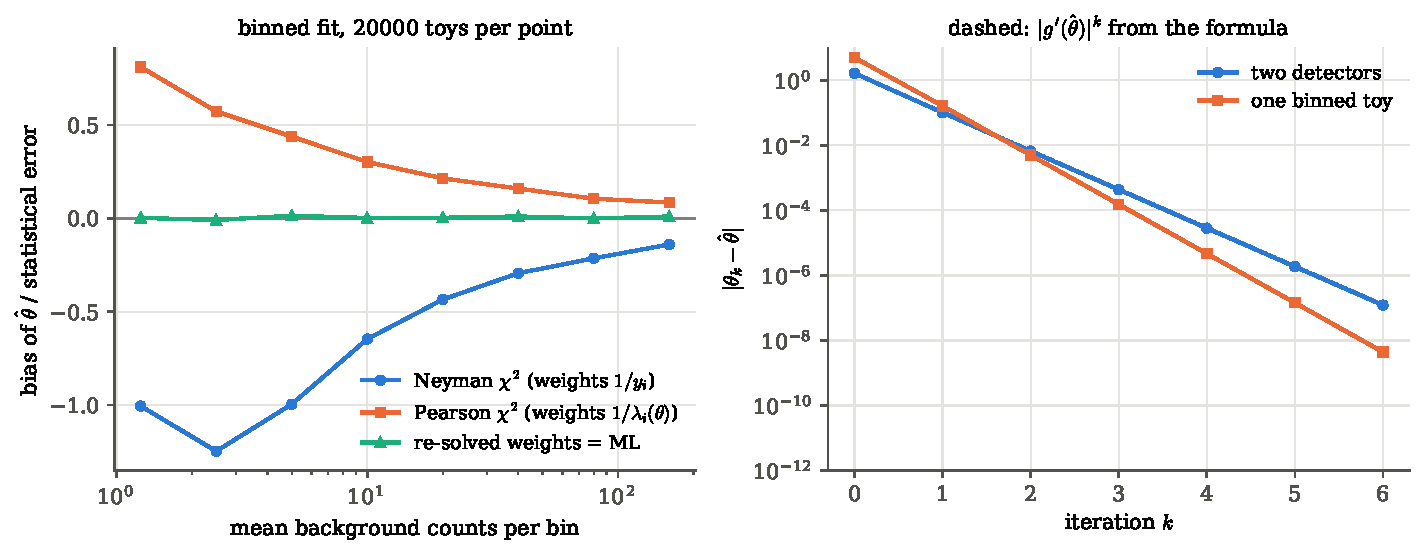
\includegraphics[width=\linewidth]{figures/chT5/iter_weights.pdf}
\caption{Left: the bias of three recipes for the total of a peak on a known
background, in units of the statistical error, against the background
counts per bin. Weights from the data (Neyman) pull the estimate low,
weights from the model minimised directly (Pearson) push it high by about
half as much, and weights re-solved from the current fit (the maximum
likelihood estimate) are unbiased at every exposure. Right: the error of the
iteration against the pass number for the two-detector example and for one
simulated spectrum; each is a straight line on the logarithmic scale,
with the slope predicted by the contraction factor $|g'(\hat\theta)|$ (dashed,
on top of the points).}
\label{T5b:fig:iter-weights}
\end{figure}

\paragraph{The same move elsewhere in the book.}
Later chapters use re-solved weights without stopping to name them. The fit
of the Hubble constant and the infall towards the Virgo cluster weights each
galaxy by the inverse of its velocity variance, which contains $H_0$ through
the distance error, and iterates the weights five times
(\cref{11c:sec:infall-sim}). The cosmic-chronometer fit has a systematic error
proportional to the model, so its covariance contains $H_0$, and it is
iterated from a starting value of $70$ (\cref{11c:sec:cc-gls}). Both are the
re-solved-weight recipe, and \eqref{T5b:eq:reweight-slope} explains why five
passes are enough: each variance changes only a little when $H_0$ moves by its
error, so the slope of the recipe is tiny. Fisher scoring, which fits CMB
parameters to a power spectrum (\cref{10a:sec:cmb-check}), is the
many-parameter form of \cref{T5b:sec:irls} below.
\subsection{Iteratively reweighted least squares}
\label{T5b:sec:irls}

The two-detector recipe is one case of a pattern that recurs throughout
statistics. Many estimators are defined as the solution of an equation of
the form
\begin{equation}
  \sum_i\psi\bigl(r_i(\theta)\bigr)\,\frac{\partial\mu_i}{\partial\theta}=0,
  \qquad r_i(\theta)=\frac{y_i-\mu_i(\theta)}{\sigma_i},
  \label{T5b:eq:estimating-eq}
\end{equation}
where $\mu_i(\theta)$ is the model's prediction for reading $y_i$, $r_i$ the
standardised residual, and $\psi$ a function that says how strongly a residual
of a given size pulls on the fit. For least squares $\psi(r)=r$: every
residual pulls in proportion to its size. Write any other $\psi$ as
$\psi(r)=w(r)\,r$, with $w(r)=\psi(r)/r$. If the weights $w(r_i)$ were constants,
\eqref{T5b:eq:estimating-eq} would be the normal equation of a weighted least
squares fit (\cref{3b:eq:normal-eq}), solved in one step. They are not
constants, because the residuals depend on $\theta$; but we can freeze them at
the current fit, solve, recompute the residuals and the weights, and repeat.
This is \newterm{iteratively reweighted least squares} (IRLS)
\cite{HollandWelsch1977,Green1984}. The two-detector recipe was IRLS with
$w_i=1/(s+b_i)$; two more examples show its range.

\paragraph{A robust mean.}
\Cref{T5a:sec:robust} introduced the Huber estimator \cite{Huber1964} for readings that are
mostly well behaved with a few wild ones. It minimises
$\sum_i\rho_k(x_i-\theta)$ with
\[
  \rho_k(r)=\begin{cases}\tfrac12r^2,&|r|\le k,\\ k|r|-\tfrac12k^2,&|r|>k,\end{cases}
  \qquad
  \psi_k(r)=\rho_k'(r)=\begin{cases}r,&|r|\le k,\\ k\,\mathrm{sign}(r),&|r|>k,\end{cases}
\]
\srcref{CasellaBerger}{(10.2.2), p.~391}: a residual pulls in proportion to
its size up to $k$, and no harder beyond. The weight is
$w(r)=\psi_k(r)/r=\min(1,k/|r|)$, so one IRLS pass for a location
($\mu_i=\theta$, $\partial\mu_i/\partial\theta=1$, $\sigma_i=1$) is a weighted mean,
\begin{equation}
  \theta_{j+1}=\frac{\sum_iw_ix_i}{\sum_iw_i},\qquad
  w_i=\min\Bigl(1,\frac{k}{|x_i-\theta_j|}\Bigr).
  \label{T5b:eq:huber-irls}
\end{equation}
A reading within $k$ of the current fit counts fully; one further out counts
in inverse proportion to its distance, so that its pull, weight times
residual, is exactly $k$.

Casella and Berger try this on eleven numbers, eight standard normal
readings and three outliers \srcref{CasellaBerger}{Ex.~10.2.5, p.~391}:
\[
  -1.28,\;-0.96,\;-0.46,\;-0.44,\;-0.26,\;-0.21,\;-0.063,\;0.39,\;3,\;6,\;9 .
\]
Their mean is $\TFiveBHubMean$, dragged up by the outliers, and their median
is $\TFiveBHubMedian$. With $k=\TFiveBHubKzero$ and the median as starting point,
\eqref{T5b:eq:huber-irls} gives $\TFiveBHubPathZero\to\TFiveBHubPathOne\to\TFiveBHubPathTwo\to\dots$
and settles at $\hat\theta=\TFiveBHubThetaKzero$ after $\TFiveBHubIters$ passes (to
$10^{-10}$). At the fixed point the eight inliers have weight one and the three
outliers have weights $1.5/|x_i-\hat\theta|$, that is $0.527$, $0.256$ and
$0.170$ (\cref{T5b:fig:irls-huber}, left).

\emph{How fast?} Use the slope formula \eqref{T5b:eq:reweight-slope}. An inlier's
weight is constant, $w_i'=0$. An outlier's weight is $w_i=k/|x_i-\theta|$, and
\begin{equation}
  w_i'\,(x_i-\theta)\eqby{1}\frac{k\,\mathrm{sign}(x_i-\theta)}{(x_i-\theta)^2}\,(x_i-\theta)
  \eqby{2}\frac{k}{|x_i-\theta|}=w_i,
  \qquad\text{so}\qquad
  g'(\hat\theta)\eqby{3}\frac{\sum_{\text{clipped}}w_i}{\sum_{\text{all}}w_i}.
  \label{T5b:eq:huber-rate}
\end{equation}
\begin{explain}
  \item $\dd|x-\theta|/\dd\theta=-\mathrm{sign}(x-\theta)$, so
        $\dd(k/|x-\theta|)/\dd\theta=k\,\mathrm{sign}(x-\theta)/(x-\theta)^2$.
  \item $\mathrm{sign}(r)\,r=|r|$.
  \item Insert into \eqref{T5b:eq:reweight-slope}; only clipped readings
        contribute to the numerator.
\end{explain}
The contraction factor is the share of the total weight carried by the
clipped readings: $(0.527+0.256+0.170)/(8+0.953)=\TFiveBHubGpFormula$, and the
ratio of successive errors in the run is $\TFiveBHubGpMeas$. A few outliers
that are far out carry little weight, and the iteration converges fast.

\emph{Why it never goes uphill.} The function $\rho_k$ depends on $r$ only
through $t=r^2$: $\rho_k=\phi(t)$ with $\phi(t)=\frac12t$ for $t\le k^2$ and
$\phi(t)=k\sqrt t-\frac12k^2$ beyond. Its slope $\phi'(t)$ is $\frac12$ and then
$k/(2\sqrt t)$, never increasing, so $\phi$ is concave and lies below each of
its tangent lines. Writing $r_{i,j}$ for the residuals at $\theta_j$, and noting
that $\phi'(r^2)=\frac12w(r)$,
\begin{align}
  \sum_i\rho_k(r_{i,j+1})
  &\relby{1}{\le}\sum_i\Bigl[\rho_k(r_{i,j})+\tfrac12w_i\bigl(r_{i,j+1}^2-r_{i,j}^2\bigr)\Bigr]\nonumber\\
  &\relby{2}{\le}\sum_i\rho_k(r_{i,j}) .
  \label{T5b:eq:huber-descent}
\end{align}
\begin{explain}
  \item The tangent line of the concave $\phi$ at $t_0=r_{i,j}^2$ lies above
        $\phi$ everywhere: $\phi(t)\le\phi(t_0)+\phi'(t_0)(t-t_0)$.
  \item $\theta_{j+1}$ minimises $\sum_iw_i(x_i-\theta)^2$ with the weights frozen
        at $\theta_j$, so $\sum_iw_ir_{i,j+1}^2\le\sum_iw_ir_{i,j}^2$.
\end{explain}
The frozen-weight quadratic touches the Huber objective at the current fit
and lies above it elsewhere, so going down the quadratic goes down the
objective. The same argument works for any $\rho$ that is a concave function of
$r^2$, and the same shape of argument, a bound that touches at the current
point, will prove that EM never goes downhill.

\Cref{T5b:fig:irls-huber}, right, shows the estimate as $k$ runs from $0$ to $10$:
from the median towards the mean, which it reaches at $k=8$ because then no
residual exceeds $k$. The table printed with this example in Casella and Berger differs at intermediate $k$; \cref{T5a:sec:huber} shows why its values cannot be minima.
The script checks every value by IRLS against a direct minimisation.

\begin{figure}[htbp]
\centering
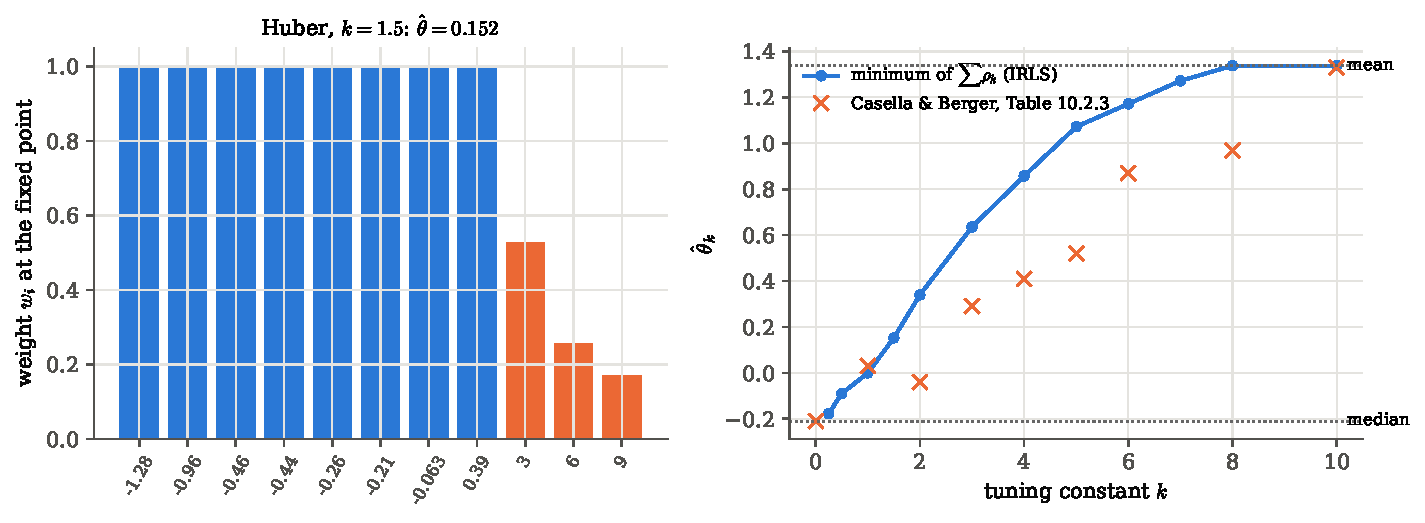
\includegraphics[width=\linewidth]{figures/chT5/irls_huber.pdf}
\caption{The Huber estimate of Casella and Berger's eleven numbers by
reweighted least squares. Left: the weights at the fixed point for
$k=1.5$; the eight readings near the centre count fully, the outliers $3$, $6$
and $9$ (orange) count less the further out they lie. Right: the estimate
against the tuning constant $k$, moving from the median ($k\to0$) to the
mean (no residual larger than $k$), with the values of Casella and Berger's
Table 10.2.3 for comparison.}
\label{T5b:fig:irls-huber}
\end{figure}

\paragraph{A decay curve with empty bins.}
A source decays with lifetime $\tau$, and we count its decays in twenty time
bins of unit width. The expected count in bin $t_i$ is
$\lambda_i=e^{a+bt_i}$, with $b=-1/\tau$: an exponential, a straight line on a
logarithmic scale. The tempting fit is a straight line through $\ln y_i$.
But late bins hold a handful of counts, some hold none, and $\ln0$ does not
exist. What does the Poisson likelihood ask for instead? With
$\eta_i=a+bt_i=\bm x_i\T\bm\beta$, $\bm x_i=(1,t_i)\T$ and $\bm\beta=(a,b)\T$,
\begin{align}
  \frac{\partial\ell}{\partial\bm\beta}
  &\eqby{1}\sum_i\Bigl(\frac{y_i}{\lambda_i}-1\Bigr)\frac{\partial\lambda_i}{\partial\bm\beta}
   \eqby{2}\sum_i(y_i-\lambda_i)\,\bm x_i,
  \qquad
  -\frac{\partial^2\ell}{\partial\bm\beta\,\partial\bm\beta\T}
   \eqby{3}\sum_i\lambda_i\,\bm x_i\bm x_i\T\equiv X\T WX,\nonumber\\
  \bm\beta_{\rm new}
  &\eqby{4}\bm\beta+(X\T WX)^{-1}X\T(\bm y-\bm\lambda)
   \eqby{5}(X\T WX)^{-1}X\T W\bm z,
  \qquad z_i=\eta_i+\frac{y_i-\lambda_i}{\lambda_i}.
  \label{T5b:eq:poisson-glm}
\end{align}
\begin{explain}
  \item The Poisson score \eqref{T5b:eq:poisson-irls}, with a vector parameter.
  \item $\partial\lambda_i/\partial\bm\beta=e^{\eta_i}\bm x_i=\lambda_i\bm x_i$.
  \item Differentiate $(y_i-\lambda_i)\bm x_i$ once more: $-\lambda_i\bm x_i\bm x_i\T$. The
        rows $\bm x_i\T$ form the matrix $X$, and $W=\diag(\lambda_i)$. The
        data $y_i$ have dropped out, so this observed curvature equals its
        average, the Fisher matrix.
  \item A Newton step (\cref{3b:sec:newton}): current point plus inverse
        curvature times score.
  \item Write $\bm\beta=(X\T WX)^{-1}X\T WX\bm\beta$ and $\bm y-\bm\lambda=WW^{-1}(\bm y-\bm\lambda)$,
        and collect: $X\bm\beta=\bm\eta$, and $W^{-1}(\bm y-\bm\lambda)$ has components
        $(y_i-\lambda_i)/\lambda_i$.
\end{explain}
So each Newton step is a weighted least-squares fit of a straight line to the
numbers $z_i$, with weights $\lambda_i$. Those are exactly the two things the
naive fit got wrong. The \emph{working response} $z_i$ is the logarithm of the
count, linearised about the current fit: the first-order Taylor expansion of
$\ln y$ about $\lambda$ is $\ln\lambda+(y-\lambda)/\lambda$, and it is finite for $y=0$. The
weight $\lambda_i$ is the inverse of $\Var(\ln y_i)\approx\Var y_i/\lambda_i^2=1/\lambda_i$ by
the delta method (\cref{3a:sec:delta}): late bins with few expected counts
count less. Here, because the curvature does not depend on the data, the
Newton step, the Fisher-scoring step of \cref{10a:sec:cmb-check} and the IRLS
step are one and the same. The slope of the recipe at the fixed point is
zero, \eqref{T5b:eq:newton-slope}, so it converges quadratically.

\pyfile[firstline=113,lastline=128,firstnumber=113]{code/chT5/21_irls.py}{Poisson regression by reweighted least squares}

\noindent Line 114 starts from a straight line through $\ln(y_i+\frac12)$, a crude
but finite guess. Each pass computes the current linear predictor $\eta_i$ and
expected counts $\lambda_i$ (lines 118--119), the working response and weights
(lines 120--121), and solves the weighted normal equations (line 122). The
script checks the result against a general-purpose minimiser of $-\ell$.

For one simulated curve with $\tau=\TFiveBPoiTau$, $\TFiveBPoiLamZero$ expected counts in
the first bin and $\TFiveBPoiNzero$ empty bins, the largest change of the
parameters falls as $\TFiveBPoiErrOne$, $\TFiveBPoiErrTwo$, $\TFiveBPoiErrThree$ over
the passes: the exponent roughly doubles each time. The fit gives
$\hat\tau=\TFiveBPoiTauIRLS\pm\TFiveBPoiTauErr$; the straight line through the
logarithms of the non-empty bins gives $\TFiveBPoiTauLog$. Over $\TFiveBPoiNtoys$
simulated curves (\cref{T5b:fig:irls-poisson}) the Poisson fit averages
$\TFiveBPoiMeanML$ with a spread of $\TFiveBPoiSdML$, while the line through
$\ln y_i$ averages $\TFiveBPoiMeanLog$ with a spread of $\TFiveBPoiSdLog$; weighting
that line by $y_i$ helps only a little ($\TFiveBPoiMeanWlog\pm\TFiveBPoiSdWlog$). The
naive fits are biased towards long lifetimes for two reasons. Dropping
empty bins keeps, in the tail, only the bins that fluctuated up, which
flattens the tail. And the logarithm is concave, so $\E\ln y<\ln\E y$, by
more in bins with fewer counts, which tilts the line. The bias, about one
and a half standard errors, is made by the recipe, not by the data.

\begin{figure}[htbp]
\centering
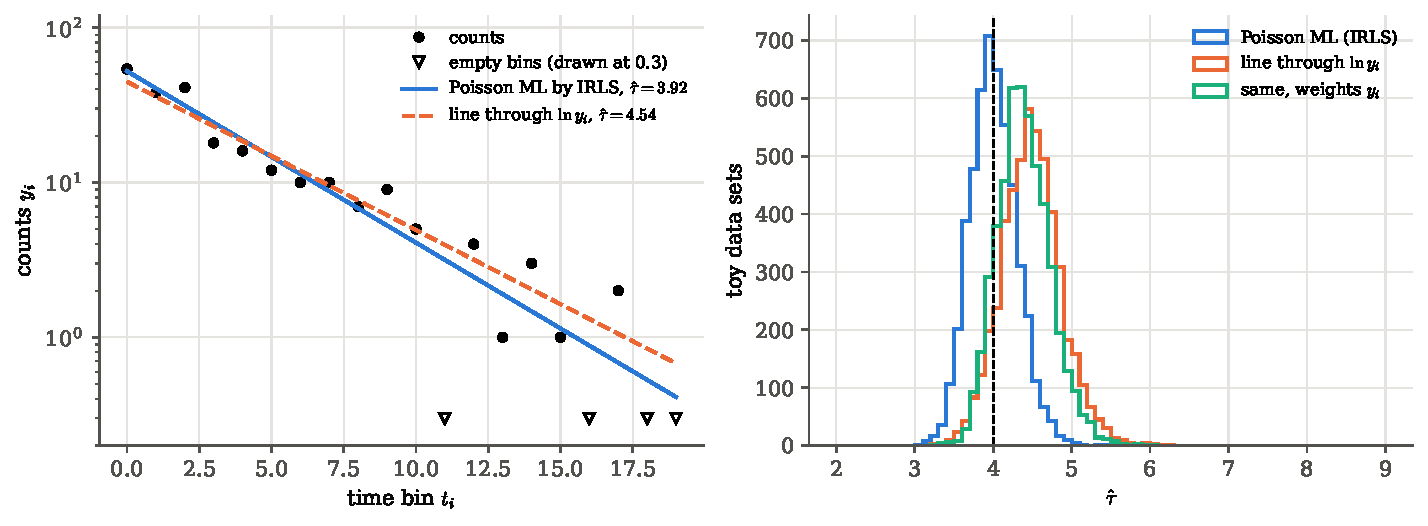
\includegraphics[width=\linewidth]{figures/chT5/irls_poisson.pdf}
\caption{Left: one simulated decay curve (points; empty bins marked by open
triangles) with the Poisson maximum-likelihood fit by reweighted least
squares (solid) and a straight line through the logarithms of the non-empty
bins (dashed). Right: the lifetimes from many simulated curves. The Poisson
fit is centred on the true value (dashed line); fits through the logarithms
are shifted to longer lifetimes and are wider.}
\label{T5b:fig:irls-poisson}
\end{figure}

This model, a count whose logarithm is linear in the parameters, is the
simplest \emph{generalised linear model}, and statistical software fits all
such models (logistic regression for yes/no outcomes is another) by exactly
this loop \cite{Green1984}.

\subsection{The EM algorithm: when the labels are missing}
\label{T5b:sec:em}

\paragraph{The problem.}
A mass spectrum between $\TFiveBEmA$ and $\TFiveBEmB$\,GeV holds $n=\TFiveBEmN$
events. A fraction $f$ of them comes from a resonance at $\mu=\TFiveBEmMu$\,GeV,
smeared by the detector into a Gaussian of width $\sigma=\TFiveBEmSig$\,GeV, as in
a diphoton search; the rest is background, which we take as flat over the
window for simplicity, with density $u=1/60$\,GeV$^{-1}$. Each event's
density is therefore the mixture
\[
  p(x\given f)=f\,\varphi(x)+(1-f)\,u,
  \qquad \varphi(x)=\frac{1}{\sqrt{2\pi}\sigma}e^{-(x-\mu)^2/2\sigma^2}.
\]
If every event carried a label saying ``signal'' or ``background'', the
estimate of $f$ would be a count: the number of signal labels divided by
$n$. The labels are missing. The likelihood $\prod_i[f\varphi(x_i)+(1-f)u]$ is a
product of sums, and its score equation $\sum_i(\varphi_i-u)/m_i=0$, with
$\varphi_i=\varphi(x_i)$ and $m_i=f\varphi_i+(1-f)u$, has no closed-form solution. When
$\mu$ and $\sigma$ are unknown too it is worse. The
\newterm{expectation--maximisation (EM) algorithm} \cite{Dempster1977}
replaces this one hard problem by a sequence of easy ones: guess the labels,
count, and repeat \mainref{pp.~143--146}.

\paragraph{Guessing the labels: Bayes for one event.}
Take one event, at mass $x_i$, and a current guess $f_k$ of the fraction.
\emph{The event.} An event was recorded at $x_i$. \emph{What could have produced
it?} Either the resonance or the background: these are the two hypotheses.
\emph{How probable was the event under each?} Under the signal hypothesis the
density at $x_i$ is $\varphi_i$, high near the peak and tiny far from it; under the
background hypothesis it is $u$, the same everywhere. \emph{Only then the
priors:} before looking at $x_i$, an event is signal with probability $f_k$.
\emph{Normalise:}
\begin{equation}
  \tau_i\equiv\Prob(\text{signal}\given x_i)
  =\frac{f_k\,\varphi_i}{f_k\,\varphi_i+(1-f_k)\,u}.
  \label{T5b:eq:em-tau}
\end{equation}
This is the \emph{E-step}: each event gets a soft label $\tau_i$ between zero and
one. An event at the peak is probably signal; an event at $150$\,GeV is
almost certainly background; an event on the shoulder of the peak is
uncertain.

\paragraph{Counting the soft labels.}
With hard labels $z_i\in\{0,1\}$ the \emph{complete-data} log-likelihood, the
one we would have with labels, is a sum of easy pieces:
\begin{equation}
  \ell_c(f,\mu,\sigma)
  \eqby{1}\sum_i\Bigl\{z_i\bigl[\ln f+\ln\varphi(x_i;\mu,\sigma)\bigr]
     +(1-z_i)\bigl[\ln(1-f)+\ln u\bigr]\Bigr\}.
  \label{T5b:eq:em-complete}
\end{equation}
\begin{explain}
  \item An event with label $z_i=1$ contributes the probability $f$ of being
        signal times the signal density; one with $z_i=0$ contributes $(1-f)u$.
        The logarithm of the product over events is the sum.
\end{explain}
We do not know the $z_i$, but we know their probabilities, so we average
$\ell_c$ over them: since $\ell_c$ is linear in each $z_i$, the average replaces
$z_i$ by $\tau_i$. The \emph{M-step} maximises this average. Setting its
derivatives to zero,
\begin{align}
  \frac{\partial}{\partial f}:\ \frac{\sum_i\tau_i}{f}-\frac{\sum_i(1-\tau_i)}{1-f}=0
  &\eqby{1}\ \Longrightarrow\ f_{k+1}=\frac1n\sum_i\tau_i,\nonumber\\
  \frac{\partial}{\partial\mu}:\ \sum_i\tau_i\frac{x_i-\mu}{\sigma^2}=0
  &\eqby{2}\ \Longrightarrow\ \mu_{k+1}=\frac{\sum_i\tau_ix_i}{\sum_i\tau_i},\nonumber\\
  \frac{\partial}{\partial\sigma}:\ \sum_i\tau_i\Bigl[-\frac1\sigma+\frac{(x_i-\mu)^2}{\sigma^3}\Bigr]=0
  &\eqby{3}\ \Longrightarrow\ \sigma^2_{k+1}=\frac{\sum_i\tau_i(x_i-\mu_{k+1})^2}{\sum_i\tau_i}.
  \label{T5b:eq:em-mstep}
\end{align}
\begin{explain}
  \item Multiply by $f(1-f)$: $(1-f)\sum\tau_i=f\sum(1-\tau_i)$, so $\sum\tau_i=fn$.
  \item $\ln\varphi=-(x-\mu)^2/2\sigma^2-\ln\sigma-\frac12\ln2\pi$; differentiate in $\mu$.
  \item Differentiate the same in $\sigma$ and multiply by $\sigma^3$.
\end{explain}
The new fraction is the average soft label: the expected number of signal
events divided by $n$. The new peak position and width are the mean and
variance of the masses, each event weighted by its probability of being
signal. Then the soft labels are recomputed with the new parameters, and so
on. The E-step is Bayes' theorem; the M-step is counting.\footnote{In
\mainref{p.~145, Ex.~9.50} the complete-data log-likelihood is printed
without its squares; it should read
$-\frac12\sum_i(1-z_i)(y_i-\mu_0)^2-\frac12\sum_iz_i(y_i-\mu_1)^2$. On p.~144 the
left-hand side $\Like(\theta^{j+1})/\Like(\theta^j)$ should be its logarithm.}

\paragraph{Why the likelihood never goes down.}
Write the hidden label of event $i$ as $z$ and any probability distribution
for it as $q_i(z)$. For one event,
\begin{align}
  \ln p(x_i\given\theta)
  &\eqby{1}\ln\sum_zp(x_i,z\given\theta)
   \eqby{2}\ln\sum_zq_i(z)\,\frac{p(x_i,z\given\theta)}{q_i(z)}\nonumber\\
  &\relby{3}{\ge}\sum_zq_i(z)\ln\frac{p(x_i,z\given\theta)}{q_i(z)}
  \equiv F_i(q_i,\theta).
  \label{T5b:eq:em-jensen}
\end{align}
\begin{explain}
  \item Marginalise over the label: $p(x\given\theta)=\sum_zp(x,z\given\theta)$, with
        $z$ = signal or background.
  \item Multiply and divide each term by $q_i(z)$.
  \item Jensen's inequality for the concave logarithm: the logarithm of an
        average is at least the average of the logarithms,
        $\ln\sum_zq_za_z\ge\sum_zq_z\ln a_z$ for weights $q_z\ge0$ adding to one.
        For two terms it says the chord of $\ln$ lies below its curve.
        Equality holds when all the $a_z$ are equal.
\end{explain}
So for any guess of the labels, $F=\sum_iF_i$ is a lower bound on the
log-likelihood. The bound touches when the ratio $p(x_i,z\given\theta)/q_i(z)$ is
the same for both labels, that is when $q_i(z)$ is proportional to
$p(x_i,z\given\theta)$: when $q_i$ is the posterior probability of the label,
which is \eqref{T5b:eq:em-tau}. Now follow one EM pass, starting from $\theta_k$.
The E-step sets $q_i$ to the posterior at $\theta_k$, so the bound touches there:
$F(q,\theta_k)=\ln\Like(\theta_k)$. In $F(q,\theta)=\sum_i\sum_zq_i(z)\ln p(x_i,z\given\theta)-\sum_i\sum_zq_i\ln q_i$,
only the first sum depends on $\theta$, and it is the averaged complete-data
log-likelihood, so the M-step maximises $F$ over $\theta$. Then
\begin{equation}
  \ln\Like(\theta_{k+1})\relby{1}{\ge}F(q,\theta_{k+1})\relby{2}{\ge}F(q,\theta_k)\eqby{3}\ln\Like(\theta_k).
  \label{T5b:eq:em-monotone}
\end{equation}
\begin{explain}
  \item The bound \eqref{T5b:eq:em-jensen} holds at every $\theta$.
  \item $\theta_{k+1}$ maximises $F(q,\cdot)$, so it does at least as well as $\theta_k$.
  \item The E-step made the bound touch at $\theta_k$.
\end{explain}
\Cref{T5b:fig:em-bound} draws it for four events: a curve that is easy to
climb is laid under the likelihood, touching at the current point; we climb
it to its top, and the likelihood there is at least as high. The proof is
\mainref{p.~144} and \srcref{CasellaBerger}{Thm.~7.2.20, p.~266} in our
notation.

\begin{figure}[htbp]
\centering
\begin{tikzpicture}
\begin{axis}[width=10cm,height=6cm,xmin=0.05,xmax=0.8,ymin=-0.3,ymax=1.25,
  xlabel={signal fraction $f$},ylabel={log-likelihood (up to a constant)},
  tick label style={font=\footnotesize},label style={font=\small},
  legend style={font=\footnotesize,at={(0.98,0.03)},anchor=south east,draw=none,fill=white},
  clip=true]
  \addplot[very thick,formblue,domain=0.05:0.8,samples=120]
    {ln(1+7*x)+ln(1+2*x)+ln(1-0.8*x)+ln(1-0.9*x)};
  \addlegendentry{$\ln\mathcal L(f)$}
  \addplot[thick,fibreorange,dashed,domain=0.05:0.8,samples=120]
    {1.167247*ln(x)+2.832753*ln(1-x)+3.349859};
  \addlegendentry{bound $F$ made at $f_0$}
  \addplot[thick,tangentgreen,dashed,domain=0.05:0.8,samples=120]
    {1.435765*ln(x)+2.564235*ln(1-x)+3.655066};
  \addlegendentry{bound $F$ made at $f_1$}
  \addplot[only marks,mark=*,mark size=1.8pt,black,forget plot]
    coordinates {(0.2,0.839137) (0.291812,1.001934) (0.358941,1.068804)};
  \addplot[only marks,mark=o,mark size=2.2pt,fibreorange,forget plot] coordinates {(0.291812,0.934638)};
  \draw[softgray,densely dotted] (axis cs:0.291812,-0.3) -- (axis cs:0.291812,1.001934);
  \draw[softgray,densely dotted] (axis cs:0.447024,-0.3) -- (axis cs:0.447024,1.099516);
  \node[font=\footnotesize,anchor=east] at (axis cs:0.195,0.86) {$f_0$};
  \node[font=\footnotesize,anchor=south east] at (axis cs:0.29,1.01) {$f_1$};
  \node[font=\footnotesize,anchor=south] at (axis cs:0.36,1.08) {$f_2$};
  \node[font=\footnotesize,anchor=west] at (axis cs:0.452,-0.2) {$\hat f$};
\end{axis}
\end{tikzpicture}
\caption{One EM pass for four events whose signal-to-background density
ratios are $8$, $3$, $0.2$ and $0.1$. At $f_0=0.2$ the E-step builds a lower bound
(orange, dashed) that touches the log-likelihood (blue). Its top, at
$f_1=0.292$ (open circle), is the M-step. The likelihood at $f_1$ lies above
the bound, so it went up. The bound built at $f_1$ (green) carries the
iteration to $f_2=0.359$, and so on towards the maximum at $\hat f=0.447$.}
\label{T5b:fig:em-bound}
\end{figure}

\paragraph{The spectrum.}
The whole E-step and M-step for the fraction fit into two lines of the script \pyname{22_em_mixture.py}.

\pyfile[firstline=50,lastline=54,firstnumber=50]{code/chT5/22_em_mixture.py}{EM for the signal fraction}

\noindent Line 53 is \eqref{T5b:eq:em-tau} for all events at once, and line 54
counts the soft labels. With the peak known and the fraction to be found,
EM started at $f=0.5$ goes $0.5\to\TFiveBEmPathOne\to\TFiveBEmPathTwo\to\TFiveBEmPathThree\to\dots$
and reaches $\hat f=\TFiveBEmFhat\pm\TFiveBEmFerr$, the root of the score equation, in
$\TFiveBEmItersA$ passes (to $10^{-10}$). The simulated spectrum held
$\TFiveBEmNsig$ signal events. With the position and width unknown as well,
started deliberately badly at $f=0.5$, $\mu=120$, $\sigma=5$, the full EM of
\eqref{T5b:eq:em-mstep} reaches $\hat f=\TFiveBEmBf$, $\hat\mu=\TFiveBEmBmu$\,GeV and
$\hat\sigma=\TFiveBEmBsig$\,GeV in $\TFiveBEmItersB$ passes, the same point a general
minimiser finds, and the log-likelihood rises at every pass
(\cref{T5b:fig:em-fit}).

\begin{figure}[htbp]
\centering
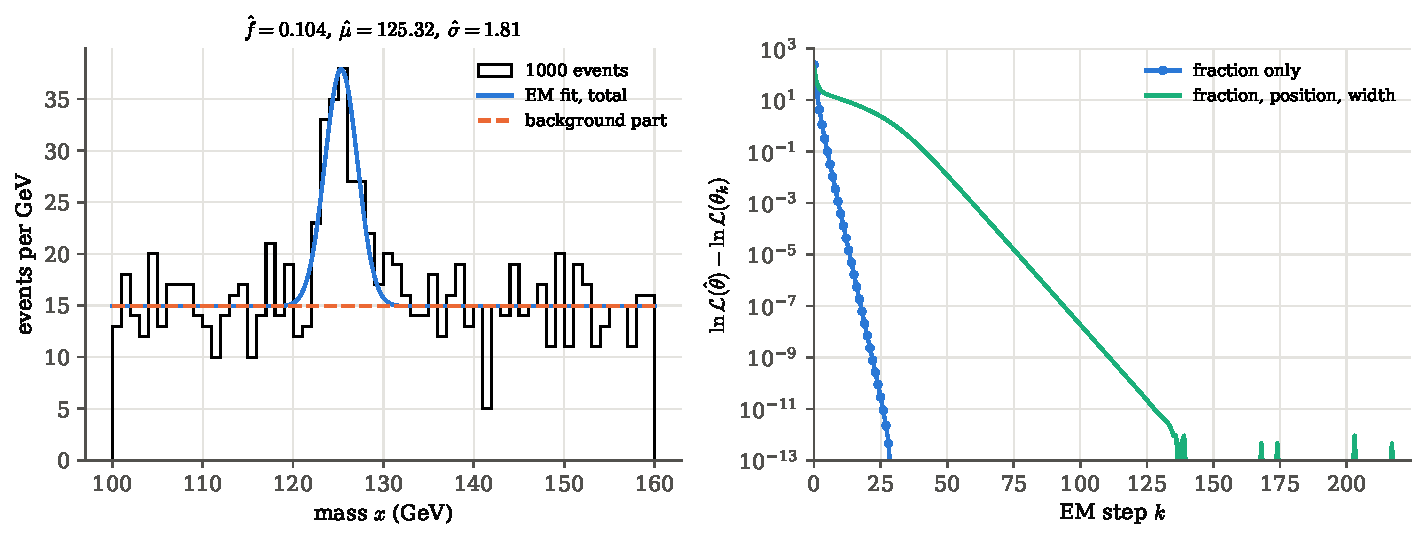
\includegraphics[width=\linewidth]{figures/chT5/em_fit.pdf}
\caption{Left: the simulated mass spectrum with the EM fit of fraction,
position and width (solid) and its background part (dashed). Right: how far
the log-likelihood is below its maximum, pass by pass, for the fit of the
fraction alone (points) and of all three parameters (line). It never
increases, as \eqref{T5b:eq:em-monotone} requires; the first falls by a
constant factor per pass, the second crawls.}
\label{T5b:fig:em-fit}
\end{figure}

\paragraph{How fast? The share of information that is missing.}
EM needed $\TFiveBEmItersA$ passes where reweighting needed a handful. Its
contraction factor can be computed. One pass is
$g(f)=\frac1n\sum_if\varphi_i/m_i$ with $m_i=f\varphi_i+(1-f)u$, so
\begin{align}
  g'(f)&\eqby{1}\frac1n\sum_i\frac{\varphi_im_i-f\varphi_i(\varphi_i-u)}{m_i^2}
        \eqby{2}\frac1n\sum_i\frac{\varphi_iu}{m_i^2},\nonumber\\
  \varphi_iu&\eqby{3}m_i\tilde m_i-f(1-f)(\varphi_i-u)^2,
  \qquad\tilde m_i\equiv(1-f)\varphi_i+fu=m_i+(1-2f)(\varphi_i-u),\nonumber\\
  g'(\hat f)&\eqby{4}1+\frac{1-2\hat f}{n}\sum_i\frac{\varphi_i-u}{m_i}-\frac{\hat f(1-\hat f)}{n}\sum_i\frac{(\varphi_i-u)^2}{m_i^2}
   \eqby{5}1-\frac{I_{\rm obs}}{I_{\rm com}} .
  \label{T5b:eq:em-rate}
\end{align}
\begin{explain}
  \item Quotient rule: $\dd m_i/\dd f=\varphi_i-u$.
  \item $\varphi_im_i-f\varphi_i(\varphi_i-u)=\varphi_i[f\varphi_i+(1-f)u-f\varphi_i+fu]=\varphi_iu$.
  \item Multiply out: $m_i\tilde m_i=f(1-f)(\varphi_i^2+u^2)+[f^2+(1-f)^2]\varphi_iu$, and
        $f^2+(1-f)^2=1-2f(1-f)$; subtracting $f(1-f)(\varphi_i-u)^2$ leaves $\varphi_iu$.
        The second form of $\tilde m_i$ follows by collecting terms.
  \item Divide the identity by $m_i^2$ and average.
  \item At the estimate the score $\sum_i(\varphi_i-u)/m_i$ vanishes. The observed
        information is $I_{\rm obs}=-\ell''(\hat f)=\sum_i(\varphi_i-u)^2/m_i^2$. The
        information with labels, from $\ln f$ for each of $nf$ signal events
        and $\ln(1-f)$ for each background event, is
        $I_{\rm com}=n/(f(1-f))$, the binomial result.
\end{explain}
The contraction factor of EM is the fraction of the information that the
missing labels take away \cite{Dempster1977}. Here it is
$\TFiveBEmRate$, and the ratio of successive errors in the run is
$\TFiveBEmRateMeas$. The same number appears in the error bars: with labels
the error on $f$ would be $1/\sqrt{I_{\rm com}}=\TFiveBEmFerrCom$, without them it
is $1/\sqrt{I_{\rm obs}}=\TFiveBEmFerr$, and $1-(\TFiveBEmFerrCom/\TFiveBEmFerr)^2$
is again the contraction factor. EM is slow exactly when the labels are hard to guess.
\Cref{T5b:fig:em-speed} shows it for peaks of different widths in the same
window: a narrow peak separates signal from background well, and EM
contracts by $\TFiveBEmRateHalf$ per pass, so six digits, which take
$\ln10^6/\ln(1/\text{factor})$ passes, need about a dozen; a peak twelve GeV wide
overlaps the background everywhere, the factor is $\TFiveBEmRateTwelve$, and
six digits take several hundred passes.

\begin{figure}[htbp]
\centering
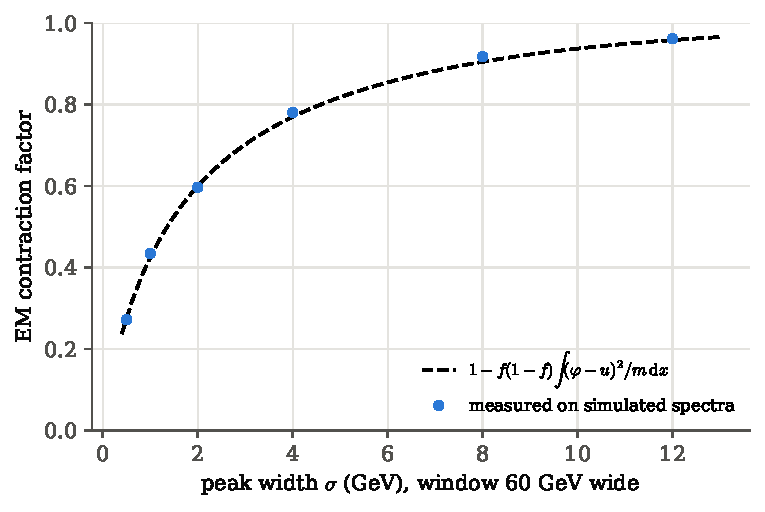
\includegraphics[width=8.5cm]{figures/chT5/em_speed.pdf}
\caption{The contraction factor of EM for the signal fraction against the
width of the peak, in a window $60$\,GeV wide with $10\%$ signal. Dashed:
the population value of $1-I_{\rm obs}/I_{\rm com}$; points: the median over
twenty simulated spectra of the measured ratio of successive errors. The
more the peak overlaps the background, the less each event says about its
own label, and the slower EM converges.}
\label{T5b:fig:em-speed}
\end{figure}

\begin{pitfall}[EM climbs, but maybe the wrong hill]
\Cref{T5b:eq:em-monotone} guarantees that the likelihood never decreases,
not that EM finds the highest maximum. It converges to a stationary point
of the likelihood under mild conditions \cite{Wu1983}
\srcref{CasellaBerger}{\S7.5.4, p.~299}, which can be a local maximum. For
mixtures there are several: a peak placed on a background fluctuation, or
the two components swapped. Start from several points, as for any
maximiser, and compare the likelihoods reached \mainref{p.~143}.
\end{pitfall}

\emph{EM or Newton?} Newton's method converges quadratically but needs second
derivatives and can step downhill far from the maximum; EM needs only the
complete-data maximisation, which is often a weighted average, and never
steps downhill, but converges linearly at the rate of missing information.
A common practice is to run EM first and finish with a few Newton steps.
The iterative unfolding of \cref{6b:sec:unf-bayes} is EM for Poisson counts in
true bins, with ``which true bin did this event come from?'' as the missing
label: its fixed point, \eqref{6b:eq:unf-fixed}, is the maximum-likelihood
condition, as \eqref{T5b:eq:em-monotone} leads us to expect.

\subsection{Stopping early on purpose}
\label{T5b:sec:early-stop}

So far the iteration was a means to an end: run it until it stops changing.
Sometimes the end point is the problem. When a detector's smearing is undone
by unfolding, the maximum-likelihood solution amplifies the noise in the
rough components of the spectrum, and \cref{6b:sec:unf-bayes} finds that a
few EM passes, stopped early, give a smaller error than running to
convergence. Why should the number of passes act like a regularisation
strength?

The simplest iteration that shows it is gradient descent on a least-squares
problem. We want $\bm\theta$ from $\bm y=A\bm\theta+\text{noise}$, and step
downhill on $\frac12|\bm y-A\bm\theta|^2$ with a small step $\omega$, starting
from $\bm\theta_0=\bm0$. In the eigenvectors of $A\T A$, with eigenvalues $s_j^2$,
each component evolves on its own:
\begin{align}
  \bm\theta_{k+1}&\eqby{1}\bm\theta_k+\omega A\T(\bm y-A\bm\theta_k),\nonumber\\
  \bm\theta_{k+1}-\hat{\bm\theta}&\eqby{2}(\Id-\omega A\T A)(\bm\theta_k-\hat{\bm\theta}),\nonumber\\
  \theta_{k,j}&\eqby{3}\bigl[1-(1-\omega s_j^2)^k\bigr]\,\hat\theta_j .
  \label{T5b:eq:landweber}
\end{align}
\begin{explain}
  \item The gradient of $\frac12|\bm y-A\bm\theta|^2$ is $-A\T(\bm y-A\bm\theta)$.
  \item Subtract the least-squares solution $\hat{\bm\theta}$, which obeys
        $A\T\bm y=A\T A\hat{\bm\theta}$ (\cref{3b:eq:normal-eq}).
  \item Along eigenvector $j$ the matrix multiplies by $1-\omega s_j^2$ at each step;
        after $k$ steps from $\bm\theta_0=\bm 0$ the error is
        $-(1-\omega s_j^2)^k\hat\theta_j$.
\end{explain}
A component with a large $s_j^2$, which the data measure well, converges in a
few steps. A component with a tiny $s_j^2$, which the data barely see and
where $\hat\theta_j$ is mostly noise, has moved only the fraction
$1-(1-\omega s_j^2)^k\approx k\omega s_j^2$ of the way. Compare the Tikhonov
(ridge) estimate, which minimises $|\bm y-A\bm\theta|^2+\tau|\bm\theta|^2$, so
$(A\T A+\tau\Id)\bm\theta=A\T\bm y$ and $\theta_{\tau,j}=s_j^2/(s_j^2+\tau)\,\hat\theta_j$.
For well-measured components both factors are near one; for poorly measured
ones, $s_j^2/\tau$ against $k\omega s_j^2$. The two filters agree when
\begin{equation}
  \tau\approx\frac{1}{\omega k}:
  \label{T5b:eq:k-tau}
\end{equation}
stopping after $k$ steps is regularisation with strength $1/(\omega k)$
(\cref{T5b:fig:filters}). More passes, weaker regularisation; running to
convergence is no regularisation at all. EM for unfolding behaves the same
way, multiplicatively instead of additively, which is why its pass count
has to be chosen with the same care as $\tau$
\cite{DAgostini1995}.

\begin{figure}[htbp]
\centering
\begin{tikzpicture}
\begin{semilogxaxis}[width=10cm,height=5.6cm,xmin=0.001,xmax=10,ymin=0,ymax=1.05,
  xlabel={how well a component is measured, $s_j^2$},ylabel={fraction of $\hat\theta_j$ kept},
  tick label style={font=\footnotesize},label style={font=\small},
  legend style={font=\footnotesize,at={(0.02,0.97)},anchor=north west,draw=none,fill=white}]
  \addplot[very thick,formblue,domain=0.001:10,samples=150] {1-(1-0.09*x)^10};
  \addlegendentry{stop after $k=10$ steps}
  \addplot[thick,formblue,dashed,domain=0.001:10,samples=150] {x/(x+1/(0.09*10))};
  \addlegendentry{Tikhonov, $\tau=1/(\omega k)$}
  \addplot[very thick,fibreorange,domain=0.001:10,samples=150] {1-(1-0.09*x)^100};
  \addlegendentry{stop after $k=100$ steps}
  \addplot[thick,fibreorange,dashed,domain=0.001:10,samples=150] {x/(x+1/(0.09*100))};
  \addlegendentry{Tikhonov, $\tau=1/(\omega k)$}
\end{semilogxaxis}
\end{tikzpicture}
\caption{How much of each component of the least-squares solution
survives, for gradient descent stopped after $k$ steps (solid; step
$\omega=0.09$) and for Tikhonov regularisation with $\tau=1/(\omega k)$ (dashed).
Well-measured components (right) are kept by both; poorly measured ones
(left), mostly noise, are suppressed by both, in nearly the same way. Ten
times more steps moves the cut ten times further to the left.}
\label{T5b:fig:filters}
\end{figure}

\paragraph{What the iterative estimators have in common.}
Every iterative recipe met so far had the same three ingredients. A best estimator
whose form needs the parameter itself: weights $1/(s+b_i)$, clipped weights,
soft labels. A map $g$ that improves a guess. And a fixed point that is the
estimator we wanted, usually the maximum-likelihood one, reached at a speed
set by $|g'|$ at the fixed point: tiny for reweighting when the model fits,
zero for Newton, the missing information for EM. The practical checks follow:
watch the ratio of successive changes, start from more than one point when
the likelihood may have several maxima, and decide whether you want the
fixed point at all.
\section{Estimators that correct their own bias}
\label{T5b:sec:bias}

\paragraph{What we already have.}
An estimator's bias is the gap between its average over repeated
experiments and the truth, and its mean squared error is the variance plus
the square of the bias (\cref{3a:sec:mse}). Some estimators are unbiased by
construction: the sample mean, the variance with $n-1$ in the denominator.
For others, \cref{3a:sec:delta} found a small systematic offset from the
curvature of a nonlinear function: $\E(1/x)\approx(1/\mu)(1+\sigma^2/\mu^2)$, above
$1/\mu$. Maximum-likelihood estimates are consistent, so their bias
disappears as the sample grows (\cref{3b:sec:consistency}), and for most
purposes that is the end of the matter.

\paragraph{When that is not enough.}
A small bias matters in two situations. When each estimate rests on few data,
a bias of order $1/n$ can be a sizeable fraction of the answer. And when
many such estimates are combined, the scatter averages down while the bias
does not, so after enough combining the bias is all that is left. In both
cases we would like to remove the bias, ideally without a formula for it,
since for a complicated estimator there is none.

\paragraph{A story with the whole trick in it.}
A GPS watch records a runner's position every ten seconds and adds up the
straight lines between the points. On a winding trail the straight lines cut
the corners, so the watch always reads short, and it reads shorter the
fewer points it uses. We cannot see the true length, but we can see how the
answer changes with the number of points: recompute the length from every
other point and see how much shorter it comes out. If we know that the
shortfall shrinks in a definite way as the points get denser, the two
answers can be extrapolated to infinitely many points, and most of the
shortfall is gone. Nothing outside the watch's own data was needed.

An estimator from $n$ readings is in the same position. Its bias usually
shrinks like $1/n$, so leaving one reading out and recomputing shows how the
answer moves when the sample shrinks, and the two answers can be
extrapolated to an infinite sample. Lifetimes are the physics version:
the decay constant $\lambda$ of a particle is estimated from $n$ measured
lifetimes $t_i$ by $\hat\lambda=1/\bar t=n/\sum_it_i$, the maximum-likelihood
estimate, and it is biased high.

\paragraph{The story in symbols: five lifetimes.}
Take $n=5$ lifetimes, $t=(0.5,\,1.0,\,1.5,\,2.0,\,3.0)$ (in some unit of time),
with sum $S=8$. The estimate is $\hat\lambda=5/8=0.625$. Leave out each lifetime
in turn and recompute with the remaining four:
\[
  \hat\lambda_{(i)}=\frac{4}{S-t_i}=0.5333,\ 0.5714,\ 0.6154,\ 0.6667,\ 0.8000,
  \qquad \bar\lambda_{(\cdot)}=\frac15\sum_i\hat\lambda_{(i)}=0.6374 .
\]
With four lifetimes the estimate is on average $0.0124$ higher than with five.
If the bias is $a/n$, going from five readings to four adds
$a/4-a/5=a/20$; so $a/20\approx0.0124$, the bias of the five-reading estimate
is $a/5\approx4\times0.0124=0.0495$, and the corrected value is
$0.625-0.0495=0.5755$. That is the \newterm{jackknife} \cite{Quenouille1956,Tukey1958}:
\begin{equation}
  \hat\lambda_{\rm JK}=n\hat\lambda-(n-1)\,\bar\lambda_{(\cdot)}
  =5(0.625)-4(0.6374)=0.5755 .
  \label{T5b:eq:jk-example}
\end{equation}
The dial is how far to extrapolate. Doing nothing leaves the full bias,
which for this estimator is exactly $\lambda/(n-1)$, a quarter of $\lambda$ at
$n=5$ (\cref{T5b:sec:bias-1n} derives it). The jackknife removes the $1/n$
part and leaves an error of order $1/n^2$. The price is a little extra
scatter, and \cref{T5b:sec:bias-price} weighs it. Lesson: a bias that
shrinks in a known way with the sample size can be measured by shrinking
the sample, and extrapolated away.

\paragraph{A picture: extrapolating in $1/n$.}
Plot the estimate against $1/n$ (\cref{T5b:fig:jk-extrapolate}). The full sample
gives one point, at $1/5$; the average of the leave-one-out estimates gives
another, at $1/4$. If the bias is proportional to $1/n$, the points lie on a
straight line that reaches the truth at $1/n=0$, an infinite sample. The
line through $(1/n,\hat\lambda)$ and $(1/(n-1),\bar\lambda_{(\cdot)})$ has slope
$(\bar\lambda_{(\cdot)}-\hat\lambda)\,n(n-1)$, so its value at zero is
$\hat\lambda-(n-1)(\bar\lambda_{(\cdot)}-\hat\lambda)$, which is \eqref{T5b:eq:jk-example}.

\begin{figure}[htbp]
\centering
\begin{tikzpicture}
\begin{axis}[width=9cm,height=5.4cm,xmin=-0.01,xmax=0.28,ymin=0.48,ymax=0.68,
  xlabel={$1/(\text{number of lifetimes used})$},ylabel={estimate of $\lambda$},
  tick label style={font=\footnotesize},label style={font=\small},
  xtick={0,0.2,0.25},xticklabels={$0$,$\tfrac15$,$\tfrac14$},
  clip=false]
  \addplot[thick,formblue,dashed,domain=0:0.25] {0.575549+(0.637363-0.625)/(0.05)*x};
  \addplot[only marks,mark=*,mark size=2pt,formblue] coordinates {(0.2,0.625) (0.25,0.637363)};
  \addplot[only marks,mark=*,mark size=2.2pt,fibreorange] coordinates {(0,0.575549)};
  \addplot[only marks,mark=o,mark size=1.6pt,softgray] coordinates
     {(0.25,0.53333) (0.25,0.57143) (0.25,0.61538) (0.25,0.66667)};
  \node[font=\footnotesize,anchor=south east] at (axis cs:0.195,0.628) {all five: $0.625$};
  \node[font=\footnotesize,anchor=west] at (axis cs:0.262,0.6374) {mean of leave-one-out: $0.637$};
  \node[font=\footnotesize,anchor=west] at (axis cs:0.262,0.552) {leave-one-out values};
  \node[font=\footnotesize,anchor=north west] at (axis cs:0.005,0.572) {jackknife: $0.576$};
\end{axis}
\end{tikzpicture}
\caption{The jackknife as an extrapolation. The estimate from all five
lifetimes (blue, at $1/5$) and the average of the five estimates with one
lifetime left out (blue, at $1/4$; the individual values are grey circles,
one of them, $0.80$, above the frame) define a straight line, which is
followed to an infinite sample at $1/n=0$ (orange).}
\label{T5b:fig:jk-extrapolate}
\end{figure}

\paragraph{One idea, many names.}
Measuring an error by changing a resolution parameter and extrapolating to
the limit is an old idea in physics and numerical analysis. Richardson
extrapolation combines a numerical derivative or integral computed with
step $h$ and with step $h/2$ so that the leading error term cancels, and
Romberg integration repeats this. Lattice field theory extrapolates results
at several lattice spacings to the continuum limit, and several volumes to
infinite volume. The jackknife is Richardson extrapolation with $1/n$ as the
step. The bootstrap estimates the same bias differently, by simulating
from the data \cite{Efron1979}, and repeating either correction gives the
\emph{iterated} bias corrections, which turn out to be the fixed-point
iterations of \cref{T5b:sec:iterative} in disguise.

Four questions follow. Why is the bias so often of order $1/n$
(\cref{T5b:sec:bias-1n})? Does the jackknife really remove it, and what does it
leave (\cref{T5b:sec:jackknife})? How does the bootstrap do it, and what does
iterating buy (\cref{T5b:sec:boot-bias})? What does correcting cost, and when is
it worth it (\cref{T5b:sec:bias-price})? The section ends where the idea is used
in research, the iterative reconstruction of CMB lensing
(\cref{T5b:sec:lens-iter}).

\subsection{Why the bias is so often of order \texorpdfstring{$1/n$}{1/n}}
\label{T5b:sec:bias-1n}

Many estimators are a smooth function of an average, $T=g(\bar x)$ with
$\bar x=\frac1n\sum_ix_i$, the $x_i$ independent with mean $\mu$ and variance
$\sigma^2$. Expand about $\mu$ and average:
\begin{align}
  \E\,g(\bar x)
  &\eqby{1}g(\mu)+g'(\mu)\,\E(\bar x-\mu)+\tfrac12g''(\mu)\,\E(\bar x-\mu)^2
     +\tfrac16g'''(\mu)\,\E(\bar x-\mu)^3+\dots\nonumber\\
  &\eqby{2}g(\mu)+\frac{g''(\mu)\,\sigma^2}{2n}+O\Bigl(\frac1{n^2}\Bigr).
  \label{T5b:eq:bias-smooth}
\end{align}
\begin{explain}
  \item Taylor expansion of $g$ about $\mu$, averaged term by term.
  \item $\E(\bar x-\mu)=0$; $\E(\bar x-\mu)^2=\Var\bar x=\sigma^2/n$; the third central
        moment of a mean of $n$ independent readings is $\mu_3/n^2$ (the cube of
        $\sum_i(x_i-\mu)$ keeps only the $n$ terms with one index, each $\mu_3$,
        divided by $n^3$), and the fourth is $3\sigma^4/n^2+O(n^{-3})$.
\end{explain}
The bias is the curvature of $g$ times the variance of the average, and that
variance is $\sigma^2/n$. A straight-line $g$ has no bias at all; a curved one
always has a bias that starts at $1/n$ and continues in powers of $1/n$. Two
examples.

\emph{The decay constant.} For exponential lifetimes $\mu=1/\lambda$ and
$\sigma^2=1/\lambda^2$, and $g(\mu)=1/\mu$ has $g''=2/\mu^3$, so the bias is
$\frac12(2\lambda^3)(1/\lambda^2)/n=\lambda/n$. Here the exact answer is available. The
sum $S=\sum_it_i$ of $n$ exponential lifetimes has the Gamma density
$\lambda^ns^{n-1}e^{-\lambda s}/(n-1)!$, so
\begin{equation}
  \E\frac1S\eqby{1}\int_0^\infty\frac1s\,\frac{\lambda^ns^{n-1}e^{-\lambda s}}{(n-1)!}\,\dd s
  \eqby{2}\frac{\lambda^n}{(n-1)!}\,\frac{(n-2)!}{\lambda^{n-1}}
  =\frac{\lambda}{n-1},
  \qquad
  \E\hat\lambda=\E\frac nS=\lambda\,\frac{n}{n-1}.
  \label{T5b:eq:lambda-bias}
\end{equation}
\begin{explain}
  \item The density of a sum of $n$ independent exponentials (the Gamma
        distribution with shape $n$, \cref{2b:sec:gamma}).
  \item $\int_0^\infty s^{n-2}e^{-\lambda s}\dd s=(n-2)!/\lambda^{n-1}$, the Gamma integral.
\end{explain}
So the bias is $\lambda/(n-1)=\lambda/n+\lambda/n^2+\dots$, whose first term is the
$\lambda/n$ of \eqref{T5b:eq:bias-smooth}. This is Cowan's (6.9)
\srcref{Cowan}{\S6.2, p.~73}: $\hat\tau=\bar t$ is unbiased for the lifetime, and
$1/\hat\tau$ is not unbiased for $1/\tau$.

\emph{The standard deviation.} The sample variance $s^2$ with $n-1$ is
unbiased, but its square root is not: $g(v)=\sqrt v$ is curved. Apply
\eqref{T5b:eq:bias-smooth} with $s^2$ in the role of the average, mean $\sigma^2$ and,
for Gaussian readings, variance $2\sigma^4/(n-1)$. With $g''(v)=-\frac14v^{-3/2}$,
the bias of $s$ is $\frac12(-\frac14\sigma^{-3})\,2\sigma^4/(n-1)=-\sigma/(4(n-1))$. The
exact factor is $\E s=c_4\sigma$ with $c_4=\sqrt{2/(n-1)}\,\Gamma(n/2)/\Gamma((n-1)/2)$;
for $n=5$, $c_4=\TFiveBCfourFive$ against $1-1/16=0.9375$ from the expansion.
Unbiasedness does not survive a nonlinear change of variable.

\subsection{The jackknife removes the \texorpdfstring{$1/n$}{1/n} term}
\label{T5b:sec:jackknife}

Let $T_n$ be any estimator computed from $n$ independent readings, with
$\E T_n=\theta+a/n+b/n^2+\dots$, where $a$ and $b$ may depend on $\theta$ but not
on $n$. Leave out reading $i$, recompute to get $T_{(i)}$, a statistic of $n-1$
readings, and average the $n$ values: $\bar T_{(\cdot)}=\frac1n\sum_iT_{(i)}$.
Casella and Berger define the jackknife estimator as
$\mathrm{JK}(T_n)=nT_n-\frac{n-1}{n}\sum_iT_{(i)}=nT_n-(n-1)\bar T_{(\cdot)}$
\srcref{CasellaBerger}{Ex.~7.66, p.~297}. Its average is
\begin{align}
  \E\,\mathrm{JK}(T_n)
  &\eqby{1}n\Bigl(\theta+\frac an+\frac b{n^2}\Bigr)-(n-1)\Bigl(\theta+\frac a{n-1}+\frac b{(n-1)^2}\Bigr)+\dots\nonumber\\
  &\eqby{2}\theta+\frac bn-\frac b{n-1}+\dots
   \eqby{3}\theta-\frac{b}{n(n-1)}+\dots
  \label{T5b:eq:jk-removes}
\end{align}
\begin{explain}
  \item Each $T_{(i)}$ is the same estimator applied to $n-1$ readings, so it has
        the same expansion with $n-1$ in place of $n$, and so does their average.
  \item The $\theta$'s give $n\theta-(n-1)\theta=\theta$; the $a$'s give $a-a=0$.
  \item $1/n-1/(n-1)=-1/(n(n-1))$.
\end{explain}
\begin{keyidea}[The jackknife removes the $1/n$ bias]
If $\E T_n=\theta+a/n+O(n^{-2})$, then $nT_n-(n-1)\bar T_{(\cdot)}$ has bias
$O(n^{-2})$, whatever $a$ is. It needs no formula for the bias, only the
ability to recompute the estimator with one reading left out. If the bias is
exactly $a/n$, the jackknife is exactly unbiased.
\end{keyidea}

\paragraph{Example: the square of a success probability.}
Casella and Berger's exercise makes the last sentence concrete. Let
$x_1,\dots,x_n$ be Bernoulli trials with success probability $\theta$, and estimate
$\theta^2$ by $T_n=\bar x^2$. With $S=\sum_ix_i$ binomial,
$\E T_n=(\Var S+(\E S)^2)/n^2=\theta^2+\theta(1-\theta)/n$: a bias of exactly $a/n$. The
leave-one-out estimate is $T_{(i)}=(S-x_i)^2/(n-1)^2$; $S$ of them have $x_i=1$ and
the other $n-S$ have $x_i=0$. So
\begin{align}
  \mathrm{JK}
  &\eqby{1}\frac{S^2}n-\frac{S(S-1)^2+(n-S)S^2}{n(n-1)}
   \eqby{2}\frac{(n-1)S^2-(n-2)S^2-S}{n(n-1)}
   =\frac{S(S-1)}{n(n-1)},\nonumber\\
  \E\,\mathrm{JK}
  &\eqby{3}\frac{\Var S+(\E S)^2-\E S}{n(n-1)}
   =\frac{n\theta(1-\theta)+n^2\theta^2-n\theta}{n(n-1)}
   =\theta^2 .
  \label{T5b:eq:jk-bernoulli}
\end{align}
\begin{explain}
  \item $nT_n=S^2/n$ and $(n-1)\bar T_{(\cdot)}=\frac{n-1}n\sum_i(S-x_i)^2/(n-1)^2$, with the
        sum split into the $S$ successes and the $n-S$ failures.
  \item Expand: $S(S-1)^2+(n-S)S^2=nS^2-2S^2+S$; put everything over $n(n-1)$.
  \item $\E[S(S-1)]=\E S^2-\E S$, with $\E S=n\theta$ and $\Var S=n\theta(1-\theta)$.
\end{explain}
The jackknife of the maximum-likelihood estimate is exactly unbiased: it is
the count of ordered pairs of successes divided by the number of ordered
pairs of trials, the natural unbiased estimate of $\theta^2$.

\paragraph{Example: the decay constant.}
For $T_n=\hat\lambda=n/S$ the bias $\lambda/(n-1)$ is not exactly $a/n$, so a remainder
is left. It can be computed exactly. Each $\hat\lambda_{(i)}=(n-1)/(S-t_i)$ is built
from $n-1$ exponentials, so by \eqref{T5b:eq:lambda-bias} with $n-1$ in place of
$n$ its average is $\lambda(n-1)/(n-2)$, and
\begin{equation}
  \E\hat\lambda_{\rm JK}\eqby{1}n\,\frac{\lambda n}{n-1}-(n-1)\,\frac{\lambda(n-1)}{n-2}
  \eqby{2}\lambda\,\frac{n^2(n-2)-(n-1)^3}{(n-1)(n-2)}
  \eqby{3}\lambda-\frac{\lambda}{(n-1)(n-2)} .
  \label{T5b:eq:jk-lambda}
\end{equation}
\begin{explain}
  \item Average of $n\hat\lambda$ minus $n-1$ times the average leave-one-out value.
  \item Common denominator.
  \item $n^3-2n^2-(n^3-3n^2+3n-1)=n^2-3n+1=(n-1)(n-2)-1$.
\end{explain}
A bias of $+\lambda/(n-1)$ has become $-\lambda/((n-1)(n-2))$: at $n=5$ from $+0.25\lambda$
to $-0.083\lambda$, at $n=10$ from $+0.111\lambda$ to $-0.014\lambda$. The simulation of
$\TFiveBLamNtoys$ experiments per sample size in \pyname{23_bias_correction.py}
finds $\TFiveBLamBiasJKFive$ and $\TFiveBLamBiasJKTen$ (\cref{T5b:fig:bias-ladder}).
The same leave-one-out values also give an error bar, the jackknife variance
of \cref{13c:sec:jackknife}, which a later chapter uses for correlation
functions measured from one sky.

\subsection{The bootstrap estimate of bias, and iterating it}
\label{T5b:sec:boot-bias}

The bootstrap of \cref{3b:sec:bootstrap} replaced the unknown distribution $F$
of the data by the empirical distribution $\hat F$, which puts probability
$1/n$ on each observed value, and simulated from it. The same move estimates
a bias. In the real world the bias is $\E_F T-\theta$. In the bootstrap world
the data come from $\hat F$, and the quantity being estimated is the same
function of $\hat F$ that $\theta$ is of $F$: the \emph{plug-in} value, which for
$\hat\lambda=1/\bar t$ is $1/\bar t$ itself, the estimate $T$. So the bootstrap
world's bias is $\E^*T^*-T$, where $T^*$ is the estimator recomputed on a
resample and $\E^*$ the average over resamples \cite{Efron1979}, and the
corrected estimator is
\begin{equation}
  T_1=T-\bigl(\E^*T^*-T\bigr)=2T-\E^*T^* .
  \label{T5b:eq:boot-bias}
\end{equation}
For a smooth function of a mean, the bootstrap world has its own version of
\eqref{T5b:eq:bias-smooth}, $\E^*g(\bar x^*)-g(\bar x)\approx g''(\bar x)\hat\sigma^2/2n$, the
true bias with $\mu,\sigma$ replaced by their estimates. The error of that
replacement is of order $1/\sqrt n$ times a term of order $1/n$, and averages
to order $1/n^2$: like the jackknife, one bootstrap correction leaves a bias
of order $1/n^2$.

\emph{A parametric version that can be done by hand.} If we trust the
exponential model, we can resample from the fitted exponential instead of
from the data. Then each resampled estimate has, by \eqref{T5b:eq:lambda-bias},
the average $\E^*T^*=cT$ with $c=n/(n-1)$, and \eqref{T5b:eq:boot-bias} gives
$T_1=(2-c)T$, whose average is $(2-c)c\lambda$. Writing $c=1+\varepsilon$ with
$\varepsilon=1/(n-1)$, $(1-\varepsilon)(1+\varepsilon)=1-\varepsilon^2$: the bias has dropped from
$\varepsilon\lambda=\lambda/(n-1)$ to $-\varepsilon^2\lambda=-\lambda/(n-1)^2$.

\emph{Iterating.} $T_1$ is itself an estimator with a bias, which the bootstrap
can estimate in the same way: recompute $T_1$ on resamples, $T_1^*=2T^*-\E^{**}T^{**}$,
where the double star marks resamples drawn from a resample. One point needs
care: in the bootstrap world the truth is still the plug-in value $T$, not
$T_1$. So the bias of $T_1$ is estimated by $\E^*T_1^*-T$, and
\begin{equation}
  T_2=T_1-\bigl(\E^*T_1^*-T\bigr)
  \eqby{1}2T-\E^*T^*-2\E^*T^*+\E^*\E^{**}T^{**}+T
  =3T-3\E^*T^*+\E^*\E^{**}T^{**}.
  \label{T5b:eq:double-boot}
\end{equation}
\begin{explain}
  \item Insert $T_1=2T-\E^*T^*$ and $\E^*T_1^*=2\E^*T^*-\E^*\E^{**}T^{**}$.
\end{explain}
This is the \newterm{iterated} (double) bootstrap \cite{HallMartin1988}. In the
parametric version every level multiplies by $c$, so $T_2=(3-3c+c^2)T$ and
$\E T_2=(1-\varepsilon+\varepsilon^2)(1+\varepsilon)\lambda=(1+\varepsilon^3)\lambda$: each level gains one more power
of $1/(n-1)$.

\emph{The fixed point behind the ladder.} What is the iteration converging
to? We are looking for the parameter value $\theta_c$ that would, on average,
produce the estimate we observed: $\theta_c+b(\theta_c)=T$, where $b(\theta)$ is the
bias when the truth is $\theta$. Written as $\theta_c=T-b(\theta_c)$, this is a
fixed-point equation, and the natural iteration is
\begin{equation}
  \theta^{(0)}=T,\qquad \theta^{(j+1)}=T-b\bigl(\theta^{(j)}\bigr).
  \label{T5b:eq:bias-fixed-point}
\end{equation}
For the decay constant $b(\theta)=\varepsilon\theta$, so $\theta^{(1)}=(1-\varepsilon)T$, the one-level
parametric bootstrap; $\theta^{(2)}=T-\varepsilon(1-\varepsilon)T=(1-\varepsilon+\varepsilon^2)T$, the two-level one. The
slope of the map is $-\varepsilon$, so by \cref{T5b:sec:contraction} it converges,
alternating in sign, to $\theta_c=T/(1+\varepsilon)=T\,(n-1)/n$. That is the exactly
unbiased estimator, since $\E[T(n-1)/n]=\lambda$ by \eqref{T5b:eq:lambda-bias}. Each
level of bootstrap is one pass of a fixed-point iteration on the bias
equation, and the iteration helps when the bias is a smooth, well-estimated
function of the parameter with $|b'|<1$. The same equation, with many parameters at once,
fixes the power spectrum of a reconstructed lensing map: its bias $N^{(1)}$ is
linear in the very spectrum being measured, so the debiased spectrum solves
$\bm c=\bm d-\mathbf K\bm c$, and \cref{T1b:sec:recon-solve} solves it both
directly and by this iteration.

\paragraph{What the simulation shows.}
\Cref{T5b:fig:bias-ladder}, left, compares the corrections over $\TFiveBLamNtoys$
simulated experiments per sample size, the bootstrap with $\TFiveBLamBone$
resamples and, for the double bootstrap, $\TFiveBLamBtwo$ second-level resamples
of each. The plain estimate follows the exact $\lambda/(n-1)$; the jackknife
follows \eqref{T5b:eq:jk-lambda}. The nonparametric bootstrap does better than
expected: at $n=10$ its bias is $\TFiveBLamBiasBootTen\pm\TFiveBLamBiasErrTen$, consistent
with zero. Iterating it does not help here. At $n=10$ the double bootstrap
is off by $\TFiveBLamBiasDbootTen\pm\TFiveBLamBiasErrDTen$, no better than one level.
At $n=5$ it misbehaves. A resample of a resample of five lifetimes can
consist of the shortest lifetime five times over, which gives a huge
$1/\bar t^{**}$, so a few experiments produce enormous corrections and the
average is dominated by them. Its median is off by only
$\TFiveBLamMedDbootFive$ and its interquartile range, $\TFiveBLamIqrDbootFive$, is
like the plain estimator's $\TFiveBLamIqrPlainFive$, but its mean is unstable.
This is the weakness of \cref{3b:sec:boot-fail} again: resampling copes badly
with statistics that a single extreme reading can control. The theorem that
each level gains a power of $1/n$ is about large $n$. The parametric ladder,
which uses the model instead of resampling, does gain a power at each level.

\begin{figure}[htbp]
\centering
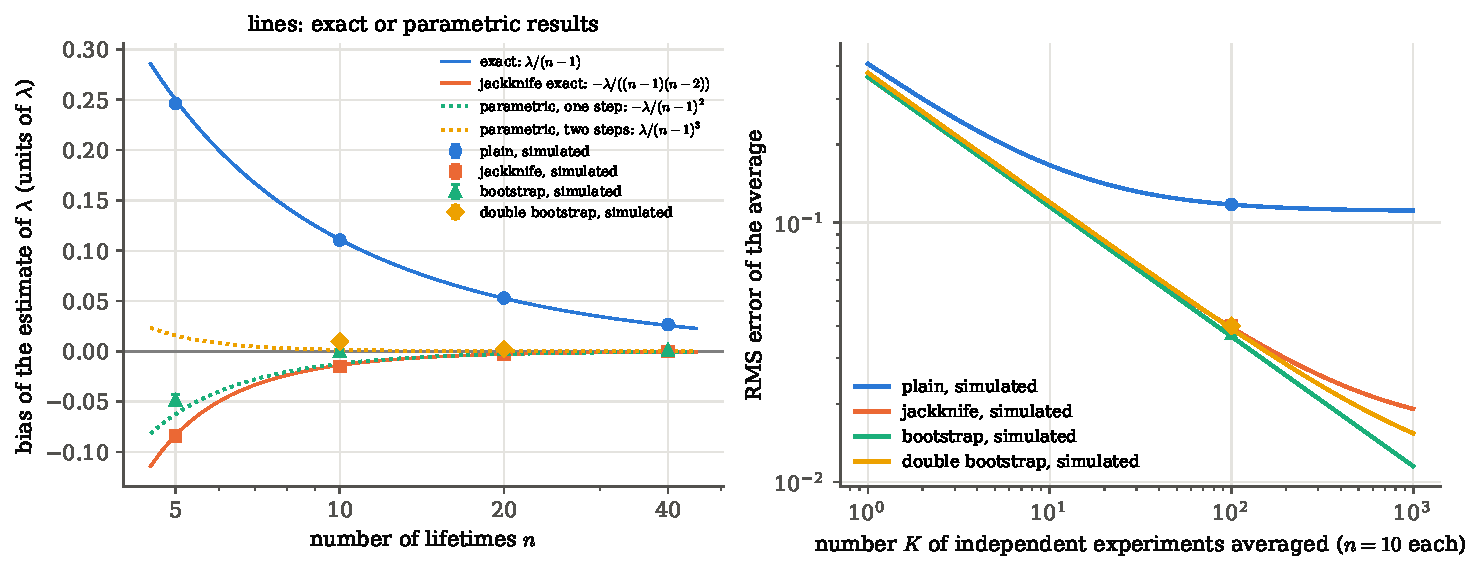
\includegraphics[width=\linewidth]{figures/chT5/bias_ladder.pdf}
\caption{Left: the bias of the decay constant estimated from $n$ lifetimes,
in units of $\lambda$, for the plain estimate and three corrections (points,
simulated; error bars are Monte Carlo errors), against the exact plain and
jackknife results and the one- and two-level parametric bootstrap (lines).
The double bootstrap at $n=5$ is off the scale and omitted. Right: the
error of the average of $K$ independent estimates, each from $n=10$
lifetimes. The scatter averages down as $1/\sqrt K$; the bias of the plain
estimate does not, and beyond $K\approx12$ it is all that is left. Points:
direct simulation at $K=100$.}
\label{T5b:fig:bias-ladder}
\end{figure}

\subsection{What a correction costs, and when it is worth it}
\label{T5b:sec:bias-price}

Removing a bias changes the estimator, and therefore its variance. By
\eqref{3a:eq:mse-decomp} the mean squared error is the variance plus the
squared bias, and a correction of order $1/n$ changes the variance at order
$1/n^2$, the same order as the squared bias it removes. Whether the error goes
down or up depends on the case.

\emph{When the correction shrinks the estimate, it wins twice.} The exactly
unbiased $T(n-1)/n$ for the decay constant has variance $((n-1)/n)^2$ times that
of $T$: smaller. The jackknife behaves similarly: at $n=10$ its mean squared
error is $\TFiveBLamMseJKTen\lambda^2$ against $\TFiveBLamMsePlainTen\lambda^2$ for the plain
estimate.

\emph{When it stretches the estimate, it can lose.} The sample standard
deviation is biased low, $\E s=c_4\sigma$ with $c_4<1$, and the unbiased version
$s/c_4$ stretches it. Since $\E s^2=\sigma^2$, $\Var s=\sigma^2(1-c_4^2)$, and
\begin{equation}
  \mathrm{MSE}(s)\eqby{1}\sigma^2(1-c_4^2)+\sigma^2(1-c_4)^2=2\sigma^2(1-c_4),
  \qquad
  \mathrm{MSE}(s/c_4)\eqby{2}\frac{\Var s}{c_4^2}=\sigma^2\Bigl(\frac1{c_4^2}-1\Bigr).
  \label{T5b:eq:sd-mse}
\end{equation}
\begin{explain}
  \item Variance plus squared bias, and $(1-c_4^2)+(1-c_4)^2=2-2c_4$.
  \item $s/c_4$ is unbiased, so its error is all variance.
\end{explain}
For $n=5$, $c_4=\TFiveBCfourFive$, and the two are $0.120\sigma^2$ and $0.132\sigma^2$:
the unbiased estimator is worse. The simulation with $\TFiveBSdNtoys$ samples
agrees ($\TFiveBSdPlainMseFive$ and $\TFiveBSdCfourMseFive$) and adds the jackknife of
$s$: it removes most of the bias ($\TFiveBSdPlainBiasFive\sigma$ becomes
$\TFiveBSdJKBiasFive\sigma$) but raises the variance from $\TFiveBSdPlainVarFive\sigma^2$ to
$\TFiveBSdJKVarFive\sigma^2$, and its mean squared error, $\TFiveBSdJKMseFive\sigma^2$, is the
largest of the three. For one experiment with a small sample, removing a
bias can make the answer worse.

\begin{pitfall}[Unbiased is not the same as better]
A bias correction trades a systematic error for extra scatter. For a single
measurement judged by its mean squared error, the trade can go either way,
and \eqref{T5b:eq:sd-mse} shows a case where it loses. Correct a bias when the
estimate will be combined with many others, or when a systematic offset
would be misread as physics; do not correct it by reflex.
\end{pitfall}

\emph{When the bias matters: combining many estimates.} Average $K$
independent estimates, each from $n$ lifetimes. The variance falls as $1/K$,
the bias stays:
\begin{equation}
  \mathrm{MSE}(K)\eqby{1}\frac{\Var\hat\lambda}{K}+b^2,\qquad
  K_{\rm cross}\eqby{2}\frac{\Var\hat\lambda}{b^2}\eqby{3}\frac{n^2}{n-2}.
  \label{T5b:eq:k-cross}
\end{equation}
\begin{explain}
  \item The average of independent estimates has the same bias and $1/K$ of
        the variance.
  \item The two terms are equal at $K_{\rm cross}$.
  \item $\Var\hat\lambda=n^2\E(1/S^2)-(\E\hat\lambda)^2$ with
        $\E(1/S^2)=\lambda^2/((n-1)(n-2))$ (the Gamma integral of
        \eqref{T5b:eq:lambda-bias} with $s^{-2}$), so
        $\Var\hat\lambda=\lambda^2n^2/((n-1)^2(n-2))$; and $b=\lambda/(n-1)$.
\end{explain}
For $n=10$, $K_{\rm cross}=12.5$, and the simulation gives $\TFiveBAvgKcross$. Average
more than about a dozen ten-event experiments and the bias of the plain
estimate dominates. At $K=\TFiveBAvgK$ its error is $\TFiveBAvgRmsPlainHundred\lambda$,
almost all bias, against $\TFiveBAvgRmsJKHundred\lambda$ after the jackknife and
$\TFiveBAvgRmsBootHundred\lambda$ after the bootstrap (\cref{T5b:fig:bias-ladder}, right).
The rule of thumb is that a $1/n$ bias matters once we average more than
about $n$ estimates, or once the bias is a sizeable fraction of the final
error bar. That is the normal situation for a power spectrum, built from
hundreds of multipoles that each have only a few modes, and for any stacked
measurement made of many small samples.

\subsection{In research: iterating a lensing reconstruction}
\label{T5b:sec:lens-iter}

The reconstruction of the CMB lensing potential in \cref{T1b:sec:recon}
combines two problems met above: an estimator whose best weights depend on
what it estimates, and a bias that has to be removed.
There we built the quadratic estimator $\hat\psi$ from pairs of temperature
modes and found that the spectrum of the reconstruction is the signal plus
two biases, $C^{\psi\psi}_L+N^{(0)}_L+N^{(1)}_L$ \eqref{T1b:eq:recon-budget}. The noise
term $N^{(0)}$ equals the normalisation of the best weights,
$N^{(0)}_L=\bigl[\int f^2/(2C^{\rm tot}_{\ell_1}C^{\rm tot}_{\ell_2})\bigr]^{-1}$
\eqref{T1b:eq:qe-mv}: the smaller the total power $C^{\rm tot}$ in the modes being
paired, the smaller the noise. For temperature we found that $N^{(0)}$
comes mostly from the chance pairing of the unlensed CMB with itself, which
no amount of cleverness can remove.

\emph{Their question.} Hirata and Seljak asked whether the quadratic estimator
is the best one can do, by writing down the full likelihood of the lensed
sky as a function of $\psi$ \cite{HirataSeljak2003T,HirataSeljak2003P}. For
temperature at the noise of Planck the answer was essentially yes. For
polarisation it was no, and the reason is a fixed point.

\emph{The mechanism.} The most sensitive polarisation estimator pairs $E$
modes with $B$ modes. Primordial $B$ modes are faint or absent, so on a
low-noise map the observed $B$ is mostly lensing: $E$ modes deflected by the
very $\psi$ we want. The $EB$ version of the noise formula has
$C^{EE,\rm tot}C^{BB,\rm tot}$ in the denominator \cite{HuOkamoto2002}, and
$C^{BB,\rm tot}$ is lensing power plus instrument noise. So the reconstruction
noise is set by the lensing signal. Now iterate. Reconstruct $\psi$; use it to
undo the lensing of the observed maps (\emph{delensing}), which removes most
of the lensing $B$ modes; the residual $B$ power is smaller, so the best
weights change and $N^{(0)}$ drops; reconstruct again with the cleaner
maps; repeat (\cref{T5b:fig:lens-iter}). The fixed point is the
maximum-likelihood $\psi$ of the full likelihood, and in the language of
\cref{T5b:sec:iterative} it is a reweighting recipe whose weights depend on the
answer through the residual $C^{BB}$. Hirata and Seljak found that the mean
squared error of the reconstruction drops by as much as a factor of two at a
noise level of $1.4\,\mu$K-arcmin and by as much as ten at $0.25\,\mu$K-arcmin,
depending on the angular scale
\cite{HirataSeljak2003P}. The temperature case differs exactly where
\cref{T1b:sec:recon} found: there $N^{(0)}$ is unlensed CMB, which delensing does
not touch.

\emph{In practice.} Modern analyses implement the iteration as a
maximum-a-posteriori reconstruction, solving for $\psi$ and the delensed
CMB together with the lensing remapping done exactly
\cite{CarronLewis2017}, and they are needed for the next generation of
low-noise polarisation experiments. Every bias of \cref{T1b:sec:recon} then
has an iterated counterpart: $N^{(0)}$ and $N^{(1)}$ must be recomputed for the
iterated estimator, by simulations that go through the same iterations as
the data. The lesson about bias corrections applies in full: the correction is
estimated from simulations that mimic the estimator, and the iteration is
stopped once the change in $\hat\psi$ is small compared with its noise.

\begin{figure}[htbp]
\centering
\begin{tikzpicture}[
  bx/.style={draw=accent,thick,rounded corners=2pt,fill=ideabg,font=\small,
             align=center,text width=30mm,minimum height=10mm},
  flow/.style={->,thick,accent}]
  \node[bx] (maps) at (0,0) {observed $E$, $B$ maps};
  \node[bx] (qe) at (4.2,0) {quadratic estimate $\hat\psi$, weights from $C^{BB,\rm tot}$};
  \node[bx] (del) at (4.2,-2.4) {delens the maps with $\hat\psi$};
  \node[bx] (res) at (0,-2.4) {residual $B$ power smaller: new weights, smaller $N^{(0)}$};
  \draw[flow] (maps) -- (qe);
  \draw[flow] (qe) -- (del);
  \draw[flow] (del) -- (res);
  \draw[flow] (res) -- (qe);
\end{tikzpicture}
\caption{The iteration of a polarisation lensing reconstruction. The noise
of the estimate depends on the $B$-mode power, most of which is produced by
the lensing being estimated; removing it with the current estimate lowers
the noise of the next one. The loop settles at the maximum-likelihood
reconstruction.}
\label{T5b:fig:lens-iter}
\end{figure}
\section{Estimators that update with every reading}
\label{T5b:sec:recursive}

\paragraph{What we already have.}
Every estimator so far took the whole data set at once. The mean adds all
the readings and divides; least squares builds $A\T\Cmat^{-1}A$ from all the rows
of the design matrix and inverts it (\cref{3b:eq:normal-eq}). If one more
reading arrives, we start again.

\paragraph{When that is not enough.}
Some data never stop arriving. A detector fires calibration pulses every
second for months; a telescope's pointing is checked against stars all
night; an online trigger must decide about each event before the next one
comes. Keeping every reading and recomputing from scratch costs memory and
time that grow without limit. Worse, the quantity may not stand still. A
photomultiplier's gain drifts with temperature; a mean over all the pulses
since the start of the run then describes the detector as it was on
average, not as it is now.

\paragraph{A story with the whole trick in it.}
A ship's navigator before satellites kept one number for the ship's
position, with an idea of how uncertain it was. Between star sightings she
advanced the position by the ship's speed and heading, and because currents
and steering errors push the ship unpredictably, her uncertainty grew with
every hour. When a star sighting came, she did not throw away her estimate
and use the sighting alone, nor ignore the sighting: she moved her position
towards it, a long way if her own estimate had grown uncertain and the
sighting was good, a little if the sighting was poor. Then the uncertainty
shrank, and the cycle began again. She never needed the log of all past
sightings, only the current position and its uncertainty.

That is what a recursive estimator does with a stream of calibration
readings: keep the current estimate and its variance; let the variance grow
by the amount the quantity can drift between readings; when a reading
arrives, move the estimate towards it by a fraction set by the two
variances. When nothing drifts, this reproduces the ordinary mean exactly,
reading by reading.

\paragraph{The story in symbols: a running mean.}
Readings $10$, $12$, $11$, $13$ arrive one at a time. Writing $m_N$ for the mean
of the first $N$, each new reading moves the mean by a fraction $1/N$ of the
\emph{surprise}, the difference between the reading and the current mean:
\begin{equation}
  m_N\eqby{1}\frac{(N-1)\,m_{N-1}+x_N}{N}
  \eqby{2}m_{N-1}+\frac1N\bigl(x_N-m_{N-1}\bigr).
  \label{T5b:eq:running-mean}
\end{equation}
\begin{explain}
  \item The first $N-1$ readings add up to $(N-1)m_{N-1}$; add the new one and
        divide by $N$.
  \item Split $(N-1)m_{N-1}/N=m_{N-1}-m_{N-1}/N$.
\end{explain}
So $m_1=10$, $m_2=10+\frac12(12-10)=11$, $m_3=11+\frac13(11-11)=11$,
$m_4=11+\frac14(13-11)=11.5$, which is $46/4$, the batch mean. The dial is the
fraction $1/N$, the \newterm{gain}: how far the estimate moves towards a new
reading. Here it shrinks as readings accumulate, which is right when the
quantity is constant, because the estimate is already backed by $N-1$
readings. It is wrong when the quantity drifts: after a thousand readings a
new one moves the estimate by a thousandth of the surprise, and the
estimate can no longer follow. On the drifting detector gain simulated in
\cref{T5b:sec:kalman}, the running mean of all readings is off by
$\TFiveBKfRmsRun$ on average, six times worse than the best recursive
estimator, whose gain stays near $\TFiveBKfKss$ for ever. Lesson: an estimate can
be updated with one number per reading, and the whole art is choosing how far
each reading moves it.

\paragraph{A picture: predict and update.}
\Cref{T5b:fig:kalman-gauss} shows one cycle when the belief about the quantity
is a Gaussian. Between readings, the quantity may drift: the belief keeps its
centre and widens (left). A reading is a second, independent Gaussian piece
of information; multiplying the two (Bayes' theorem with the widened belief
as the prior) gives a narrower Gaussian whose centre lies between them,
closer to whichever is narrower (right).

\begin{figure}[htbp]
\centering
\begin{tikzpicture}
\begin{axis}[name=ax1,width=6.6cm,height=4.6cm,xmin=-3,xmax=5,ymin=0,ymax=1.2,
  xlabel={gain $g$ (shifted, scaled)},ytick=\empty,title={predict: the belief widens},
  tick label style={font=\scriptsize},label style={font=\small},title style={font=\small},
  legend style={font=\scriptsize,draw=none,fill=none,at={(0.98,0.97)},anchor=north east}]
  \addplot[very thick,formblue,domain=-3:5,samples=120] {exp(-x^2/(2*0.5^2))/(0.5*sqrt(2*pi))};
  \addlegendentry{after reading $t-1$}
  \addplot[very thick,formblue,dashed,domain=-3:5,samples=120] {exp(-x^2/(2*1.0^2))/(1.0*sqrt(2*pi))};
  \addlegendentry{before reading $t$}
\end{axis}
\begin{axis}[at={(ax1.east)},anchor=west,xshift=8mm,width=6.6cm,height=4.6cm,xmin=-3,xmax=5,ymin=0,ymax=1.2,
  xlabel={gain $g$ (shifted, scaled)},ytick=\empty,title={update: multiply by the reading},
  tick label style={font=\scriptsize},label style={font=\small},title style={font=\small},
  legend style={font=\scriptsize,draw=none,fill=none,at={(0.98,0.97)},anchor=north east}]
  \addplot[thick,formblue,dashed,domain=-3:5,samples=120] {exp(-x^2/(2*1.0^2))/(1.0*sqrt(2*pi))};
  \addlegendentry{prediction, var.\ $1$}
  \addplot[thick,fibreorange,domain=-3:5,samples=120] {exp(-(x-2)^2/(2*0.75^2))/(0.75*sqrt(2*pi))};
  \addlegendentry{reading, var.\ $0.56$}
  \addplot[very thick,tangentgreen,domain=-3:5,samples=120] {exp(-(x-1.28)^2/(2*0.36))/(0.6*sqrt(2*pi))};
  \addlegendentry{updated, var.\ $0.36$}
\end{axis}
\end{tikzpicture}
\caption{One cycle of the Kalman filter for a Gaussian belief. Left: between
readings the quantity may drift, so the variance grows by the drift variance
(here from $0.25$ to $1$) while the centre stays. Right: the prediction
(variance $1$, centre $0$) and a reading at $2$ with variance $0.5625$ combine into a
Gaussian with variance $1/(1+1/0.5625)=0.36$ and centre $0+0.64\times2=1.28$:
the gain $K=1/(1+0.5625)=0.64$ moves the estimate most of the way towards the
better of the two.}
\label{T5b:fig:kalman-gauss}
\end{figure}

\paragraph{One idea, many names.}
Updating an estimate by a fraction of the surprise is everywhere. The
running mean and its exponentially weighted cousin, which keeps the gain
fixed, are used in every control room. Recursive least squares updates a
fit point by point. The \newterm{Kalman filter} \cite{Kalman1960}, which
navigated the Apollo spacecraft, is the general Gaussian version with a
drifting state. In Bayesian language all of them are one rule: today's
posterior is tomorrow's prior, the sequential use of Bayes' theorem that
\cref{ch:05} makes central. The mathematics is the algebra of Gaussians,
because a Gaussian belief multiplied by a Gaussian likelihood is again
Gaussian, so the whole belief is carried by two numbers.

We first make the running mean and variance exact and safe in
floating-point arithmetic (\cref{T5b:sec:running}), then extend the update
to least-squares fits (\cref{T5b:sec:rls}), and finally let the quantity
drift (\cref{T5b:sec:kalman}).

\subsection{The running mean and variance}
\label{T5b:sec:running}

\eqref{T5b:eq:running-mean} gives the mean exactly. For the variance we need
the running sum of squared deviations, $M_N=\sum_{i\le N}(x_i-m_N)^2$, so that
$s_N^2=M_N/(N-1)$. When a reading arrives, the mean moves, so every old
deviation changes. How does the sum change? Write $\delta=x_N-m_{N-1}$ for the
surprise; by \eqref{T5b:eq:running-mean}, $m_N-m_{N-1}=\delta/N$ and
$x_N-m_N=\delta(N-1)/N$. Then
\begin{align}
  M_N&\eqby{1}\sum_{i<N}(x_i-m_{N-1})^2+(N-1)(m_{N-1}-m_N)^2+(x_N-m_N)^2\nonumber\\
     &\eqby{2}M_{N-1}+\frac{(N-1)\,\delta^2}{N^2}+\frac{(N-1)^2\,\delta^2}{N^2}
      \eqby{3}M_{N-1}+\frac{N-1}{N}\,\delta^2\nonumber\\
     &\eqby{4}M_{N-1}+(x_N-m_{N-1})(x_N-m_N).
  \label{T5b:eq:welford}
\end{align}
\begin{explain}
  \item For the old readings write $x_i-m_N=(x_i-m_{N-1})+(m_{N-1}-m_N)$ and
        square; the cross term is $2(m_{N-1}-m_N)\sum_{i<N}(x_i-m_{N-1})=0$, because
        deviations from their own mean add up to zero. The new reading adds
        its own term.
  \item Insert $m_N-m_{N-1}=\delta/N$ and $x_N-m_N=\delta(N-1)/N$.
  \item $(N-1)/N^2+(N-1)^2/N^2=(N-1)N/N^2$.
  \item $\delta\cdot\delta(N-1)/N$ is the surprise before the update times the
        surprise after it.
\end{explain}
This is \newterm{Welford's update} \cite{Welford1962}: one pass, two stored
numbers, and nothing but small differences multiplied together.

\emph{Why not the textbook formula?} The sum of squares can also be written as
$\sum x_i^2-(\sum x_i)^2/N$, which also needs only two running sums. In exact
arithmetic the two are identical. In a computer they are not. The script
\pyname{24_recursive.py} reads $N=\TFiveBWelN$ values of a frequency counter at
$1$\,GHz with $1$\,Hz of jitter. Each $x_i^2$ is about $10^{18}$, and a double-precision
number carries sixteen significant digits, so each square is rounded by
about $100$; the difference of the two sums, which should be $N$ times one, is
the difference of two numbers near $10^{23}$ and keeps none of its digits.
The textbook formula returns a variance of $\TFiveBWelNaive$\,Hz$^2$. Welford's update
returns $\TFiveBWelVar$, against $\TFiveBWelTwo$ from two passes with accurate
summation: a relative error of $\TFiveBWelErr$. Subtracting the current mean
before squaring is what saves it.

\pyfile[firstline=35,lastline=38,firstnumber=35]{code/chT5/24_recursive.py}{Welford's running mean and variance}

\paragraph{Readings of different quality.}
If reading $N$ has variance $\sigma_N^2$, weight it by $w_N=1/\sigma_N^2$. The weighted
mean of \cref{3a:sec:weighted} updates the same way. With $P_N=\sum_{i\le N}w_i$, the
total weight (the inverse of the variance of the mean),
\begin{equation}
  P_N=P_{N-1}+w_N,\qquad
  m_N=m_{N-1}+\frac{w_N}{P_N}\bigl(x_N-m_{N-1}\bigr),
  \label{T5b:eq:running-wmean}
\end{equation}
by the same algebra as \eqref{T5b:eq:running-mean} with $N-1$ replaced by $P_{N-1}$.
Precisions add, and the gain is the new reading's share of the total
precision. For equal weights it is $1/N$.

\subsection{Recursive least squares}
\label{T5b:sec:rls}

A straight-line calibration $y=a+bx$ is fitted to points that arrive one at a
time. After $N$ points the least-squares solution (unit weights for
simplicity) is $\hat{\bm\theta}_N=P_NA_N\T\bm y_N$ with $P_N=(A_N\T A_N)^{-1}$, where row
$i$ of $A_N$ is $\bm a_i\T=(1,x_i)$ (\cref{3b:eq:normal-eq}). A new point adds one
row: $A_{N+1}\T A_{N+1}=P_N^{-1}+\bm a\bm a\T$, with $\bm a$ the new row. Inverting
a matrix plus a rank-one term is the Sherman--Morrison formula, which
\cref{11c:sec:cc-gls} checks by multiplication:
$(M+\bm a\bm a\T)^{-1}=M^{-1}-M^{-1}\bm a\bm a\T M^{-1}/(1+\bm a\T M^{-1}\bm a)$.
With $\bm k\equiv P_N\bm a/(1+\bm a\T P_N\bm a)$, the \emph{gain vector},
\begin{align}
  P_{N+1}&\eqby{1}P_N-\bm k\,\bm a\T P_N,
  \qquad P_{N+1}\bm a\eqby{2}\bm k,\nonumber\\
  \hat{\bm\theta}_{N+1}&\eqby{3}P_{N+1}\bigl(P_N^{-1}\hat{\bm\theta}_N+\bm a\,y\bigr)
   \eqby{4}(\Id-\bm k\bm a\T)\hat{\bm\theta}_N+\bm k\,y
   =\hat{\bm\theta}_N+\bm k\,\bigl(y-\bm a\T\hat{\bm\theta}_N\bigr).
  \label{T5b:eq:rls}
\end{align}
\begin{explain}
  \item Sherman--Morrison with $M=P_N^{-1}$.
  \item $P_N\bm a-\bm k\,(\bm a\T P_N\bm a)=\bm k(1+\bm a\T P_N\bm a)-\bm k\,\bm a\T P_N\bm a=\bm k$.
  \item $A_{N+1}\T\bm y_{N+1}=A_N\T\bm y_N+\bm a\,y$, and $A_N\T\bm y_N=P_N^{-1}\hat{\bm\theta}_N$.
  \item $P_{N+1}P_N^{-1}=\Id-\bm k\bm a\T$ by the first line, and $P_{N+1}\bm a=\bm k$.
\end{explain}
The fit moves by the gain vector times the surprise $y-\bm a\T\hat{\bm\theta}_N$,
the new point's residual from the current line, exactly as the running mean
did. Nothing is approximate: the script starts from the exact fit to the
first two points, feeds in the other $\TFiveBRlsN-2$ one by one, and after
every point compares with the batch solution; the largest difference over
the whole stream is $\TFiveBRlsMaxDiff$, rounding error.

\pyfile[firstline=63,lastline=68,firstnumber=63]{code/chT5/24_recursive.py}{Recursive least squares for a straight line}

\subsection{The Kalman filter: a quantity that drifts}
\label{T5b:sec:kalman}

\paragraph{The model.}
A detector's gain $g_t$ wanders slowly: from one calibration reading to the
next it changes by a random amount $w_t$ with mean zero and variance $q$, a
random walk. Each calibration reading measures the current gain with noise:
$y_t=g_t+v_t$, with $v_t$ of variance $r$. In the simulation $\sqrt q=\TFiveBKfSq$ (the
gain changes by $0.2\%$ per reading) and $\sqrt r=\TFiveBKfSr$ (each reading is good
to $5\%$). Both kinds of noise are taken Gaussian and independent. We carry a
Gaussian belief about the gain, mean $m_{t-1}$ and variance $P_{t-1}$, after reading
$t-1$.

\emph{Predict.} The next gain is $g_t=g_{t-1}+w_t$. Its mean is unchanged and its
variance is the sum of two independent variances:
\begin{equation}
  m_t^-=m_{t-1},\qquad P_t^-=P_{t-1}+q .
  \label{T5b:eq:kf-predict}
\end{equation}

\emph{Update.} The reading $y_t$ arrives. By Bayes' theorem the new belief is
the prediction times the likelihood of the reading, $\exp[-(y_t-g)^2/2r]$, as a
function of $g$. Take $-2\ln$ of the product and collect powers of $g$:
\begin{align}
  \frac{(g-m_t^-)^2}{P_t^-}+\frac{(y_t-g)^2}{r}
  &\eqby{1}g^2\Bigl(\frac1{P_t^-}+\frac1r\Bigr)-2g\Bigl(\frac{m_t^-}{P_t^-}+\frac{y_t}r\Bigr)+\text{const}
   \eqby{2}\frac{(g-m_t)^2}{P_t}+\text{const},\nonumber\\
  \frac1{P_t}&=\frac1{P_t^-}+\frac1r,\qquad
  m_t\eqby{3}P_t\Bigl(\frac{m_t^-}{P_t^-}+\frac{y_t}{r}\Bigr)
     \eqby{4}m_t^-+K_t\,\bigl(y_t-m_t^-\bigr),\qquad
  K_t=\frac{P_t^-}{P_t^-+r}.
  \label{T5b:eq:kf-update}
\end{align}
\begin{explain}
  \item Expand both squares; terms without $g$ go into the constant.
  \item Complete the square: $Ag^2-2Bg=A(g-B/A)^2-B^2/A$, with $A=1/P_t$ and
        $B/A=m_t$.
  \item Read off the centre $B/A$.
  \item With $P_t=P_t^-r/(P_t^-+r)$:
        $m_t=(r\,m_t^-+P_t^-y_t)/(P_t^-+r)=m_t^-+P_t^-(y_t-m_t^-)/(P_t^-+r)$.
\end{explain}
The precisions add, as for the weighted mean, and the estimate moves towards
the reading by the \emph{Kalman gain} $K_t$, which is the prediction's
variance divided by the total: near one when the prediction is poor, near
zero when the reading is poor. The new variance is
$P_t=(1-K_t)P_t^-=P_t^-r/(P_t^-+r)$. The same completion of the square gives the
Gaussian posterior of \cref{5b:sec:conjugate} with one reading.

\pyfile[firstline=83,lastline=92,firstnumber=83]{code/chT5/24_recursive.py}{The Kalman filter for a drifting gain}

\noindent Line 85 is the prediction \eqref{T5b:eq:kf-predict}, lines 86--87 the gain and the
update of the mean, line 88 the update of the variance. The script writes the
variance as $P^-r/(P^-+r)$ rather than $(1-K)P^-$: the two are equal, but with
a very large starting variance $1-K$ is the difference of two numbers close to
one, and the second form avoids that cancellation.

\paragraph{No drift: the running mean, again.}
With $q=0$ and a starting variance so large that the prior carries no
information, $1/P_0\to0$, the precisions simply add: $1/P_t=t/r$. Then
$K_t=P_{t-1}/(P_{t-1}+r)=(r/(t-1))/(r/(t-1)+r)=1/t$, and \eqref{T5b:eq:kf-update} is the
running mean \eqref{T5b:eq:running-mean}. The script confirms it reading by reading
on a stream of $\TFiveBKfT$, to $\TFiveBKfRunDiff$.

\paragraph{With drift: a gain that stops shrinking.}
With $q>0$ the variance no longer falls to zero. Each prediction adds $q$, each
update removes a fraction. The variance settles where the two balance, a
fixed point of the map $P^-\mapsto P^-r/(P^-+r)+q$, which is itself a
fixed-point iteration of \cref{T5b:sec:iterative}. Writing $M$ for the
settled prediction variance,
\begin{align}
  M&\eqby{1}\frac{Mr}{M+r}+q
  \quad\Longleftrightarrow\quad
  M^2\eqby{2}qM+qr
  \quad\Longleftrightarrow\quad
  M\eqby{3}\frac{q+\sqrt{q^2+4qr}}{2},\nonumber\\
  K_\infty&\eqby{4}\frac{M}{M+r}\approx\sqrt{\frac qr},\qquad
  P_\infty\eqby{5}\frac{Mr}{M+r}\approx\sqrt{qr}\qquad(q\ll r).
  \label{T5b:eq:kf-steady}
\end{align}
\begin{explain}
  \item The prediction variance after an update and a prediction equals
        itself.
  \item Multiply by $M+r$: $M^2+Mr=Mr+qM+qr$.
  \item The positive root of the quadratic.
  \item For $q\ll r$, $M\approx\sqrt{qr}\ll r$, so $M/(M+r)\approx M/r$.
  \item The updated variance; again $M\ll r$.
\end{explain}
In the steady state the filter is $m_t=m_{t-1}+K_\infty(y_t-m_{t-1})$: an
exponentially weighted average in which reading $t-j$ counts with weight
$K_\infty(1-K_\infty)^j$. Its memory is about $1/K_\infty\approx\sqrt{r/q}$ readings: the
number of readings over which the drift, $\sqrt{q}$ per reading in a random
walk, grows as large as the noise averaged over the same readings. For our
detector $K_\infty=\TFiveBKfKss$, a memory of $\TFiveBKfMem$ readings, and the error is
$\sqrt{P_\infty}=\TFiveBKfPss$, about $(qr)^{1/4}$.

\paragraph{The rivals.}
Two simpler estimators are the obvious alternatives. The running mean of all
readings so far ignores the drift. A \emph{trailing window} averages the
last $W$ readings; how wide should it be? The estimate at time $t$ has two
independent errors. The noise of $W$ averaged readings has variance $r/W$. And
the window's average gain lags the current gain:
$g_t-\frac1W\sum_{j=0}^{W-1}g_{t-j}=\frac1W\sum_{l=0}^{W-2}(W-1-l)\,w_{t-l}$, since the
increment $w_{t-l}$ separates $g_t$ from the $W-1-l$ older gains $g_{t-l-1},\dots,g_{t-W+1}$.
So
\begin{equation}
  \text{error}^2(W)\eqby{1}\frac rW+\frac q{W^2}\sum_{m=1}^{W-1}m^2\approx\frac rW+\frac{qW}3,
  \qquad
  W^*\eqby{2}\sqrt{\frac{3r}q},\qquad
  \text{error}^2(W^*)\eqby{3}2\sqrt{\frac{rq}3}.
  \label{T5b:eq:window}
\end{equation}
\begin{explain}
  \item Independent increments: the variance of the lag is $q/W^2$ times the
        sum of the squared coefficients, and $\sum_{m=1}^{W-1}m^2\approx W^3/3$.
  \item Set the derivative $-r/W^2+q/3$ to zero.
  \item Both terms equal $\sqrt{rq/3}$ at $W^*$.
\end{explain}
For our detector $W^*=\TFiveBKfWtheory$ readings and the error is $\TFiveBKfRmsWtheory$,
slightly worse than the Kalman filter's $\TFiveBKfPss$. The simulation, $\TFiveBKfR$
streams of $\TFiveBKfT$ readings each, with the first $\TFiveBKfBurn$ discarded, measures
all of them (\cref{T5b:fig:kalman-track,T5b:fig:kalman-rms}). The Kalman filter
is off by $\TFiveBKfRms$ on average, as \eqref{T5b:eq:kf-steady} predicts. The best
trailing window, found by trying every width, has $W=\TFiveBKfWbest$ and an error of
$\TFiveBKfRmsWbest$, $\TFiveBKfGain\%$ larger; the filter wins on $\TFiveBKfWinFrac\%$ of the
streams. The running mean of all readings is off by $\TFiveBKfRmsRun$: it is biased
by the drift, and more data make it worse, not better.

\begin{figure}[htbp]
\centering
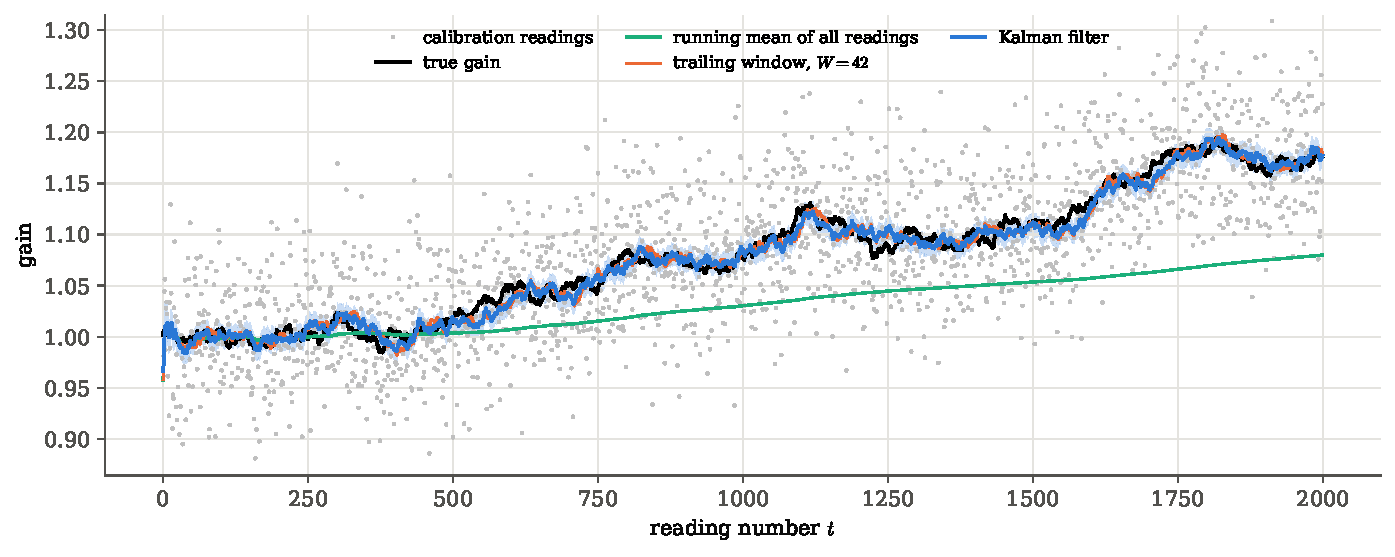
\includegraphics[width=\linewidth]{figures/chT5/kalman_track.pdf}
\caption{One simulated stream of calibration readings (grey dots) of a gain
that wanders as a random walk (black). The running mean of all readings
(green) falls behind the drift and never catches up. A trailing window of
the best width (orange) and the Kalman filter (blue, with its $\pm1\sigma$ band)
both follow it; the filter is slightly closer, with no window to choose.}
\label{T5b:fig:kalman-track}
\end{figure}

\begin{figure}[htbp]
\centering
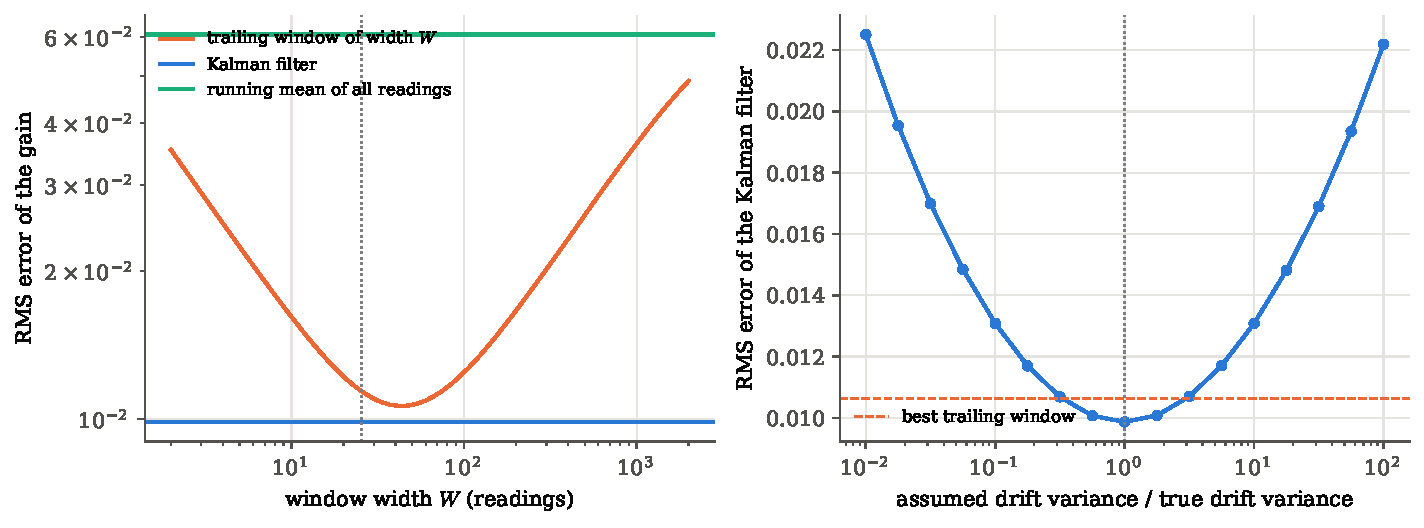
\includegraphics[width=\linewidth]{figures/chT5/kalman_rms.pdf}
\caption{Left: the error of a trailing window against its width (orange):
narrow windows are noisy, wide ones lag. Its minimum is above the error of
the Kalman filter (blue); the running mean of all readings (green) is six
times worse. The dotted line marks the filter's memory $1/K_\infty$. Right: the
error of the Kalman filter when it is told a drift variance that is wrong by
the factor on the axis. A factor of ten either way costs about a third.}
\label{T5b:fig:kalman-rms}
\end{figure}

\paragraph{What it needs.}
The filter needed $q$ and $r$. The noise $r$ of a calibration reading is usually
known from the calibration itself. The drift $q$ is rarely known, but the
filter is forgiving (\cref{T5b:fig:kalman-rms}, right): telling it a drift
variance ten times too small or too large raises its error from $\TFiveBKfRms$ to
$\TFiveBKfRmsQtenth$ and $\TFiveBKfRmsQten$. A wrong guess of the drift is equivalent to a
wrong window width, and both are cured the same way: estimate it from the
data.

\begin{inpractice}[How research uses recursive estimators]
Our filter tracks one number with known noise and drift. Real tracking
problems carry a state vector (gain, offset, temperature coefficient), a
model of how it evolves, and covariance matrices $Q$ and $R$; the predict and
update steps are the matrix versions of
\eqref{T5b:eq:kf-predict}--\eqref{T5b:eq:kf-update}, with the gain
$K=P^-H\T(HP^-H\T+R)^{-1}$ for readings $\bm y=H\bm g+\bm v$
\cite{Kalman1960}. $Q$ and $R$ are fitted by maximising the likelihood of the
surprises $y_t-m_t^-$, which the filter delivers as independent Gaussians with
variance $P_t^-+r$. When the whole stream is available afterwards, a backward
pass (the Kalman smoother) uses later readings as well, and its error is
smaller than the filter's. The same recursion fits particle tracks in a
tracking detector, hit by hit, and follows instrument gains through long
observing campaigns.
\end{inpractice}

\paragraph{Iterative or recursive?}
The two families look alike, since both repeat an update, but they answer
different questions. An iterative estimator repeats on the \emph{same}
data until a self-consistent answer stops changing. A recursive estimator
does one update per \emph{new} reading and never revisits the old ones.
The Kalman filter's variance settling to its steady state is where the two
meet: a recursion whose variance runs to a fixed point.
\section{A field guide: which estimator, when}
\label{T5b:sec:field-guide}

\paragraph{What we already have.}
Six questions about a problem each point to a family of estimators
(\cref{T5a:sec:six-questions}), and a table records what each estimator assumes
and what it optimises (\cref{T5a:tab:taxonomy}). Three more families have
joined them: estimators that iterate to a
self-consistent answer, estimators that remove their own bias, and
estimators that update with each reading.

\paragraph{When that is not enough.}
A real analysis rarely asks one question. A power spectrum from a masked
map is a parameter in the covariance, estimated at hundreds of multipoles,
with weights that need the spectrum itself, and it will be averaged into
bands. The answers interact, some questions should come first, and each
choice has a price that is worth stating before committing to it.

\paragraph{A story with the whole trick in it.}
A good mechanic facing a car that will not start does not try every repair
in the manual. She asks questions in an order: is there fuel, is there a
spark, does the starter turn. Each answer rules out a whole branch, the
cheap questions come first, and the repair at the end follows from the
answers. She also knows what each repair costs and what it can break.
Choosing an estimator works the same way. We ask, in order, where the
parameter lives, what we know about the noise, whether the recipe needs
its own answer, what else we know, how the data arrive, and how the
estimate will be used; the estimator is assembled from the answers, and
its cost is checked by simulation.

The roadmap figure (\cref{T5a:fig:roadmap}) listed the questions and the family
each answer points to. \Cref{T5b:fig:decision} turns them into a
procedure that can be followed: the first three questions are a tree that ends
in the form of the estimator, and the other four are modifiers asked of
whatever form came out. \Cref{T5b:tab:field-guide} lists situations with the
estimator each calls for, what it assumes, what it costs, and where the book
develops it. The six cases after them are worked in the order of the questions.

\begin{figure}[htbp]
\centering
\begin{tikzpicture}[
  d/.style={draw=formblue,thick,rounded corners=2pt,fill=white,align=left,
            font=\small,text width=52mm,minimum height=9mm,inner sep=3pt},
  f/.style={draw=fibreorange!80!black,thick,rounded corners=2pt,fill=white,
            align=left,font=\small,text width=66mm,minimum height=9mm,inner sep=3pt},
  m/.style={draw=tangentgreen!70!black,thick,rounded corners=2pt,fill=white,
            align=left,font=\small,text width=100mm,minimum height=9mm,inner sep=3pt},
  yes/.style={->,thick,tangentgreen!70!black},
  no/.style={->,thick,softgray},
  bracketline/.style={thick,fibreorange!80!black}]
  \node[d] (d1) at (0,0)    {1.\ Is $\theta$ in the scatter of the data rather than in their mean?};
  \node[d] (d2) at (0,-2)   {2.\ Is the full law of the noise known?};
  \node[d] (d3) at (0,-4)   {3.\ Are only some facts about the noise known?};
  \node[d] (d4) at (0,-6)   {Nothing is known beyond the data themselves.};
  \node[f] (f1) at (6.6,0)  {quadratic estimator, noise bias subtracted};
  \node[f] (f2) at (6.6,-2) {write the likelihood and maximise it (MVUE if one exists)};
  \node[f] (f3) at (6.6,-4) {mean and covariance: BLUE;\\ a few wild readings: Huber, median;\\ a few moments: method of moments};
  \node[f] (f4) at (6.6,-6) {resample the data: bootstrap};
  \foreach \i in {1,2,3} \draw[yes] (d\i.east) -- (f\i.west);
  \foreach \i/\j in {1/2,2/3,3/4} \draw[no] (d\i.south) -- (d\j.north);
  \draw[yes] (d4.east) -- (f4.west);
  \node[m] (m1) at (3.3,-8.5)  {4.\ Does the best recipe need $\theta$ itself (weights, labels, a fiducial)?
      Iterate it to a fixed point (IRLS, EM, Newton); check $|g'|<1$ and several starts.};
  \node[m] (m2) at (3.3,-10.5) {5.\ A trustworthy prior, or many similar parameters?
      Add the prior (Bayes estimator, Wiener filter) or shrink.};
  \node[m] (m3) at (3.3,-12.5) {6.\ Do the data stream in?
      Update instead of recomputing (running mean, RLS); a drifting $\theta$ calls for a Kalman filter.};
  \node[m] (m4) at (3.3,-14.5) {7.\ Will the estimate be averaged with many others, or is $n$ small?
      Remove the $1/n$ bias (jackknife, bootstrap) and check that the mean squared error does not grow.};
  \node[m] (end) at (3.3,-16.8) {Before trusting the result, simulate data from the assumed model and check the bias,
      the scatter and the coverage of the error bars.};
  \draw[bracketline] (f1.east) -- ++(4mm,0) coordinate (c1);
  \draw[bracketline] (f2.east) -- ++(4mm,0) coordinate (c2);
  \draw[bracketline] (f3.east) -- ++(4mm,0) coordinate (c3);
  \draw[bracketline] (f4.east) -- ++(4mm,0) coordinate (c4);
  \draw[bracketline] (c1) -- (c4);
  \draw[->,thick,fibreorange!80!black] (c4) |- (m1.east);
  \foreach \i/\j in {1/2,2/3,3/4} \draw[->,thick,tangentgreen!70!black] (m\i.south) -- (m\j.north);
  \draw[->,thick,tangentgreen!70!black] (m4.south) -- (end.north);
\end{tikzpicture}
\caption{The operational procedure for choosing an estimator, drawn from the
questions of the chapter roadmap (\cref{T5a:fig:roadmap}). Top: a tree. Green
arrows answer yes, grey arrows answer no and lead to the next question, and every
branch ends in the form of the estimator (orange). Bottom: four
modifiers, each asked of whatever form came out, in order. A yes adds an
ingredient to the recipe and the procedure goes on to the next question. The
last box is not optional.}
\label{T5b:fig:decision}
\end{figure}

\begin{table}[htbp]
\centering
\caption{Situations and the estimators they call for.}
\label{T5b:tab:field-guide}
\small
\begin{tabularx}{\linewidth}{@{}>{\raggedright}p{25mm}>{\raggedright}p{23mm}>{\raggedright}X>{\raggedright}X>{\raggedright\arraybackslash}p{21mm}@{}}
\toprule
situation & estimator & assumes & costs & where\\
\midrule
Gaussian readings, known errors & weighted mean, least squares & known $\sigma_i$ & nothing & \cref{3a:sec:weighted,3b:sec:least-squares}\\
full noise law, a complete sufficient statistic & minimum-variance unbiased & the full law & rarely available in closed form & \cref{3b:sec:recipe-best}\\
full noise law, large $n$ & maximum likelihood & the full law & biased at order $1/n$ & \cref{3b:sec:mle}\\
a few moments known as functions of $\theta$ & method of moments & those moments only & less efficient than ML; a good starting point for iterations & \cref{3b:sec:mom}\\
only mean and covariance of the noise known & BLUE & linear model & inefficient for heavy tails & \cref{T5a:sec:blue}\\
counts, few per bin & Poisson ML (re-solved weights) & Poisson law & an iteration; never weights $1/y_i$ & \cref{3b:sec:poisson,T5b:sec:fixed-ml}\\
a few wild readings & Huber or median, by IRLS & most readings well behaved & a little efficiency; choice of $k$ & \cref{T5a:sec:robust,T5b:sec:irls}\\
$\theta$ in the covariance & quadratic estimator & Gaussian field, known noise & noise bias to subtract; needs a fiducial & \cref{T5a:sec:quadratic}\\
prior information & Bayes estimator, Wiener filter & a trustworthy prior & biased if the prior is wrong & \cref{T5a:sec:bayes-risk}\\
many similar parameters & shrinkage & exchangeable parameters & each estimate biased & \cref{T5a:sec:stein}\\
weights need $\theta$ & fixed-point iteration, IRLS & contraction, $|g'|<1$ & iterations; may not converge & \cref{T5b:sec:iterative}\\
hidden labels, mixtures & EM & a complete-data model & slow when labels are unclear; local maxima & \cref{T5b:sec:em}\\
ill-posed inversion & regularisation or stopping early & smooth truth & bias towards the start & \cref{6b:sec:unf-tikhonov,T5b:sec:early-stop}\\
small $n$, estimate to be combined & jackknife or bootstrap correction & bias in powers of $1/n$ & more variance & \cref{T5b:sec:bias}\\
stream, constant $\theta$ & running mean, Welford, RLS & nothing new & nothing & \cref{T5b:sec:running,T5b:sec:rls}\\
stream, drifting $\theta$ & Kalman filter & drift and noise variances & needs $q$, $r$ & \cref{T5b:sec:kalman}\\
\bottomrule
\end{tabularx}
\end{table}

\subsection{Six cases}
\label{T5b:sec:cases}

Each case follows the order of reasoning of the Monty Hall problem
(\cref{ch:01}): what was observed, what we know about how it was produced, the
candidate estimators one at a time with the reason for or against each, and
only then the choice.

\paragraph{Case 1: counts on a background.}
\emph{The data.} A search counts events in a signal window in several
detectors or bins; each has a background expectation $b_i$ known from
sidebands, and the expected signal $s\,\epsilon_i$ differs between them through
the efficiency $\epsilon_i$. \emph{What do we know?} Counts are Poisson: the
noise law is known exactly, and its variance is the unknown mean.
\emph{The candidates.} Background-subtracted counts averaged with equal
weights ignore that some channels are cleaner. Weights $1/n_i$ from the
observed counts favour channels that fluctuated low, the Neyman bias
of \cref{T5b:sec:fixed-ml}. Minimising Pearson's $\chi^2$ directly pushes the
estimate up. Weights $1/(s\epsilon_i+b_i)$ re-solved from the current estimate
converge to the Poisson maximum-likelihood estimate, which question 4 told us
to expect. \emph{The choice:} the Poisson likelihood, maximised by re-solved
weights or by any maximiser, and an interval from the likelihood as in
\cref{4b:sec:fc-poisson} when the counts are small.

\paragraph{Case 2: the angular power spectrum of the CMB.}
\emph{The data.} A map, decomposed into $a_{\ell m}$, with instrument noise of
known spectrum $N_\ell$. \emph{What do we know?} The parameter $C_\ell$ is the
variance of the $a_{\ell m}$: their mean is zero whatever $C_\ell$ is. So
question 1 already decides: no linear combination of the data can see
$C_\ell$, and the estimator is quadratic. \emph{The candidates.} The plain
average of $|a_{\ell m}|^2$ over $m$ includes the noise variance, a bias equal to
$N_\ell$, which is why $\hat C_\ell=\frac1{2\ell+1}\sum_m|a_{\ell m}|^2-N_\ell$ subtracts it
(\cref{7b:eq:noise-bias}). On a masked sky the modes are coupled, and the
best quadratic weights depend on $C_\ell$ itself (question 4): either a fiducial
spectrum is used, or the estimate is iterated with its own output as the
fiducial. Question 7 matters too: each $\hat C_\ell$ at low $\ell$ rests on
$2\ell+1$ modes, so any nonlinear function of it, such as $\ln\hat C_\ell$ or
$1/\hat C_\ell$, carries a bias of order $1/(2\ell+1)$ that does not average away
over many multipoles (\cref{T5b:sec:bias-price}). \emph{The choice:} the
unbiased quadratic estimator (a pseudo-$C_\ell$ with its mode-coupling
correction, \cref{8b:sec:master}, or the quadratic maximum-likelihood
estimator of \cref{T5a:sec:quadratic}), with the noise bias subtracted, and
nonlinear functions of it left to the likelihood instead of being averaged.

\paragraph{Case 3: photometry with cosmic rays.}
\emph{The data.} Twenty exposures of a star, each giving a flux. \emph{What do
we know?} Most exposures have Gaussian noise from photon counting and
read-out; a few are hit by cosmic rays, which only ever \emph{add} charge.
This is laboratory C of \cref{T5a:sec:questions}, with a one-sided
contamination. \emph{The candidates.} The mean is pulled up by every hit and
never pulled down, so it is biased, not merely inefficient. The median is
robust but throws away about a third of the information when there are no
hits. The Huber estimator, computed by reweighted least squares with $k$
about one and a half standard deviations (\cref{T5b:sec:irls}), keeps
almost all the information and limits the pull of each hit to $k$; the
popular \emph{sigma clipping}, which repeatedly discards readings more than a
few standard deviations from the current mean, is the same fixed-point
iteration with weights that jump from one to zero. Because the hits are
one-sided, even a robust estimator keeps a small upward bias, of order the
fraction of hits times $k$. \emph{The choice:} Huber by IRLS, with $k$ and the
remaining bias checked on simulated exposures with the observed hit rate.

\paragraph{Case 4: many band powers.}
\emph{The data.} Fifty band powers of a spectrum, each with its own error.
\emph{What do we know?} Each is a fine estimate on its own, but neighbouring
bands of a smooth spectrum are similar (question 5). \emph{The candidates.}
Shrinking every band towards a smooth fit lowers the total squared error of
the fifty, as James and Stein showed (\cref{T5a:sec:stein}), but makes each
band biased towards the fit. If the band powers are the input to a
cosmological fit, that bias is harmful: the likelihood already combines the
bands with the right weights, and shrinking would pull the result towards
the smooth model assumed in the shrinkage. If the purpose is a picture or a
denoised spectrum, shrinkage is the right tool. \emph{The choice} depends on
the use: unbiased band powers with their covariance for inference,
shrinkage for display or for a first look.

\paragraph{Case 5: a detector's calibration, streamed.}
\emph{The data.} A calibration pulse every second, each measuring the gain
with a known noise. \emph{What do we know?} The gain may drift with
temperature, slowly but without a known law. \emph{The candidates.} The
running mean of all pulses is exact if nothing drifts and biased if anything
does (\cref{T5b:sec:kalman}). A trailing window of the right width works,
but the width has to be tuned. The Kalman filter with a random-walk drift
needs the drift variance, can estimate it from its own surprises, and beat
the best window on every simulated stream. \emph{The choice:} the Kalman filter
for live monitoring; the Kalman smoother, which also uses later pulses, when
the calibration is applied afterwards.

\paragraph{Case 6: the lensing potential.}
\emph{The data.} A CMB map in temperature and polarisation. \emph{What do we
know?} Lensing correlates modes that would be independent on an unlensed
sky: $\psi$ lives in the off-diagonal part of the covariance (question 1), so
the estimator is quadratic in the map, and its spectrum carries the biases
$N^{(0)}$ and $N^{(1)}$ (\cref{T1b:sec:recon}). \emph{The candidates.} The
quadratic estimator with the Hu--Okamoto weights is optimal at first order
and fast. Its biases must be removed (question 7), by formulas checked on
simulations and by the realisation-dependent $N^{(0)}$ of \cref{T1b:sec:recon}. For polarisation at low
noise its weights depend on the lensing $B$ modes it is estimating
(question 4), and the iterated reconstruction of \cref{T5b:sec:lens-iter}
reaches noise levels the quadratic estimator cannot. \emph{The choice:} the
quadratic estimator for temperature and for noisy polarisation; the
iterative or maximum-a-posteriori reconstruction for deep polarisation
maps; in both cases bias subtraction calibrated on simulations that pass
through the same pipeline.

\paragraph{What the cases share.}
No case needed an exotic estimator. Each needed the questions asked in the
right order, and in four of the six the decisive question was one the data
alone cannot answer: what the noise is, whether the parameter drifts, how
the estimate will be used. The final box of \cref{T5b:fig:decision} applied
in every case: when the estimator is chosen, simulate data under the
assumptions that chose it and measure its bias and its scatter.

\begin{recap}
\begin{itemize}[leftmargin=1.2em,itemsep=1pt]
\item When the best weights need the parameter, iterate $\theta_{k+1}=g(\theta_k)$. It
      converges when $|g'(\theta^*)|<1$, linearly with that factor per pass;
      Newton has $g'=0$ and converges quadratically. For two detectors,
      $11\to9.444\to9.349\to9.343$, with factor $0.065$.
\item Re-solved weights $1/\lambda_i(\theta)$ for counts land on the Poisson score
      equation: the maximum-likelihood estimate. Weights from the data
      (Neyman) bias low, Pearson's minimisation biases high by about half as
      much.
\item IRLS solves $\sum_i w(r_i)r_i\,\partial\mu_i/\partial\theta=0$ by weighted least squares:
      Huber's robust mean (rate = share of weight on clipped points, never
      uphill) and Poisson regression (working response $\eta+(y-\lambda)/\lambda$,
      weights $\lambda$; equal to Newton and to Fisher scoring).
\item EM: soft labels by Bayes' theorem, then count. Jensen's inequality
      makes the likelihood rise at every pass; the rate is the fraction of
      information the missing labels take away, $1-I_{\rm obs}/I_{\rm com}$.
\item Stopping an iteration after $k$ passes regularises like Tikhonov with
      $\tau\approx1/(\omega k)$.
\item A smooth function of a mean is biased by $g''\sigma^2/2n$; $1/\bar t$ by
      exactly $\lambda/(n-1)$. The jackknife $nT-(n-1)\bar T_{(\cdot)}$ removes the $1/n$
      term; the bootstrap $2T-\E^*T^*$ does too; iterating is a fixed-point
      iteration of the bias equation. A correction can raise the mean
      squared error; it pays when more than about $n$ estimates are averaged.
\item Recursive estimators update by a gain times the surprise: running
      mean (gain $1/N$), Welford's variance, RLS by Sherman--Morrison, and the
      Kalman filter (predict: variances add; update: precisions add), whose
      gain settles at $\approx\sqrt{q/r}$ and beats the best moving window.
\item Choosing an estimator: ask where $\theta$ lives, what the noise is, whether
      the recipe needs $\theta$, what else is known, how the data arrive and how
      the result will be used; then check by simulation.
\end{itemize}
\end{recap}
\section*{Chapter summary}
\label{T5b:sec:summary}
\addcontentsline{toc}{section}{Chapter summary}

\begin{center}
\small
\begin{tabularx}{\linewidth}{@{}>{\raggedright}p{30mm}>{\raggedright}X>{\raggedright\arraybackslash}p{30mm}@{}}
\toprule
concept & what it means in practice & where it is used\\
\midrule
the questions that choose an estimator & where $\theta$ lives, what the noise is, prior, how many parameters, stream, self-dependence, use of the result & every analysis; the field guide, \cref{T5b:sec:field-guide}\\
best linear unbiased estimator & weights $(A\T C^{-1}A)^{-1}A\T C^{-1}$: needs only the mean and covariance of the noise & generalised least squares in \cref{11c:sec:cc-gls}\\
Bayes risk, Wiener filter & average error over a prior; Gaussian prior and noise give the Wiener filter & priors in \cref{ch:05}; filtered maps \\
shrinkage (James--Stein) & many similar means estimated together beat one-by-one ML in total squared error & hierarchical models in \cref{ch:05}\\
robust (Huber, median) & bounded pull of each reading; computed by IRLS & outlier-prone readings; robust summaries in \cref{12b:sec:robust}\\
quadratic estimator, noise bias & a parameter in the covariance needs a quadratic estimator; noise adds a bias to subtract & $\hat C_\ell$ in \cref{7b:eq:noise-bias}; \cref{8a:sec:noise-bias}; lensing \cref{T1b:sec:recon}\\
fixed-point iteration, contraction factor & repeat $\theta\to g(\theta)$; converges if $|g'(\theta^*)|<1$, one digit per $1/\log_{10}(1/|g'|)$ passes & re-solved weights in \cref{11c:sec:infall-sim}\\
re-solved Poisson weights & weights $1/\lambda_i(\theta)$ recomputed until fixed: the Poisson ML estimate & binned fits; \cref{3b:sec:poisson}\\
IRLS & frozen weights, weighted least squares, repeat; Newton and Fisher scoring as special cases & Fisher scoring in \cref{10a:sec:cmb-check}\\
EM algorithm & soft labels by Bayes, then count; likelihood never falls; rate $=1-I_{\rm obs}/I_{\rm com}$ & iterative unfolding, \cref{6b:sec:unf-bayes}\\
stopping early & $k$ passes act like regularisation of strength $\approx1/(\omega k)$ & choosing the number of unfolding iterations, \cref{6b:sec:unf-bayes}\\
$1/n$ bias & a curved function of a mean is biased by $g''\sigma^2/2n$ & any nonlinear summary of few data\\
jackknife bias correction & $nT-(n-1)\bar T_{(\cdot)}$ removes the $1/n$ term & jackknife errors in \cref{13c:sec:jackknife}\\
bootstrap bias correction, iterated & $2T-\E^*T^*$; $3T-3\E^*T^*+\E^{**}T^{**}$; fixed-point view of the bias equation & with the bootstrap of \cref{3b:sec:bootstrap}\\
price of a correction & variance may rise; worth it when more than $\sim n$ estimates are averaged & band powers, stacked measurements\\
running mean, Welford & update by a gain times the surprise; subtract the mean before squaring & running averages of Markov chains, \cref{9a:fig:running}\\
recursive least squares & Sherman--Morrison update, identical to the batch fit & streamed calibration fits\\
Kalman filter & predict (variances add), update (precisions add); gain $\approx\sqrt{q/r}$ for a drifting quantity & monitoring detector gains\\
iterative lensing reconstruction & delens, re-estimate: noise falls when $B$ modes are lensing-dominated & CMB lensing, \cref{T1b:sec:recon}\\
\bottomrule
\end{tabularx}
\end{center}

\section*{Reading the literature}
\label{T5b:sec:reading}
\addcontentsline{toc}{section}{Reading the literature}

\begin{itemize}[leftmargin=1.2em,itemsep=2pt]
\item L. Wasserman, \emph{All of Statistics}, ch.~8 (the bootstrap, with the
      jackknife in its appendix) and \S9.13 (Newton--Raphson and the EM
      algorithm).
\item G. Casella and R. L. Berger, \emph{Statistical Inference}, \S7.2.4 (EM,
      with its monotonicity theorem), \S7.5.4, Exercise 7.66 (the jackknife),
      \S10.1.4 (bootstrap standard errors), \S10.2 (robustness, M-estimators and
      the Huber estimator).
\item G. Cowan, \emph{Statistical Data Analysis}, ch.~6--7: the bias of
      maximum-likelihood estimators and least squares with binned data.
\item Linear, Bayes and shrinkage estimators: \cite{Stein1956,JamesStein1961,EfronMorris1973,EfronMorris1975,EfronMorris1977};
      robust estimation: \cite{Huber1964,Hampel1974}; quadratic estimators of
      a power spectrum: \cite{Tegmark1997QML}.
\item Iteration: EM \cite{Dempster1977} and its convergence \cite{Wu1983};
      reweighted least squares \cite{HollandWelsch1977,Green1984}; iterative
      deconvolution and unfolding \cite{Richardson1972,Lucy1974,DAgostini1995}.
\item Bias correction: the jackknife \cite{Quenouille1956,Tukey1958}, the
      bootstrap \cite{Efron1979} and its iteration \cite{HallMartin1988}.
\item Recursive estimation: \cite{Welford1962,Kalman1960}.
\item Lensing reconstruction beyond the quadratic estimator:
      \cite{HirataSeljak2003T,HirataSeljak2003P,CarronLewis2017}.
\end{itemize}
  